\documentclass[]{article}
\usepackage{lmodern}
\usepackage{amssymb,amsmath}
\usepackage{ifxetex,ifluatex}
\usepackage{fixltx2e} % provides \textsubscript
\ifnum 0\ifxetex 1\fi\ifluatex 1\fi=0 % if pdftex
  \usepackage[T1]{fontenc}
  \usepackage[utf8]{inputenc}
\else % if luatex or xelatex
  \ifxetex
    \usepackage{mathspec}
  \else
    \usepackage{fontspec}
  \fi
  \defaultfontfeatures{Ligatures=TeX,Scale=MatchLowercase}
\fi
% use upquote if available, for straight quotes in verbatim environments
\IfFileExists{upquote.sty}{\usepackage{upquote}}{}
% use microtype if available
\IfFileExists{microtype.sty}{%
\usepackage{microtype}
\UseMicrotypeSet[protrusion]{basicmath} % disable protrusion for tt fonts
}{}
\usepackage[margin=1in]{geometry}
\usepackage{hyperref}
\hypersetup{unicode=true,
            pdftitle={final\_analysis},
            pdfborder={0 0 0},
            breaklinks=true}
\urlstyle{same}  % don't use monospace font for urls
\usepackage{color}
\usepackage{fancyvrb}
\newcommand{\VerbBar}{|}
\newcommand{\VERB}{\Verb[commandchars=\\\{\}]}
\DefineVerbatimEnvironment{Highlighting}{Verbatim}{commandchars=\\\{\}}
% Add ',fontsize=\small' for more characters per line
\usepackage{framed}
\definecolor{shadecolor}{RGB}{248,248,248}
\newenvironment{Shaded}{\begin{snugshade}}{\end{snugshade}}
\newcommand{\AlertTok}[1]{\textcolor[rgb]{0.94,0.16,0.16}{#1}}
\newcommand{\AnnotationTok}[1]{\textcolor[rgb]{0.56,0.35,0.01}{\textbf{\textit{#1}}}}
\newcommand{\AttributeTok}[1]{\textcolor[rgb]{0.77,0.63,0.00}{#1}}
\newcommand{\BaseNTok}[1]{\textcolor[rgb]{0.00,0.00,0.81}{#1}}
\newcommand{\BuiltInTok}[1]{#1}
\newcommand{\CharTok}[1]{\textcolor[rgb]{0.31,0.60,0.02}{#1}}
\newcommand{\CommentTok}[1]{\textcolor[rgb]{0.56,0.35,0.01}{\textit{#1}}}
\newcommand{\CommentVarTok}[1]{\textcolor[rgb]{0.56,0.35,0.01}{\textbf{\textit{#1}}}}
\newcommand{\ConstantTok}[1]{\textcolor[rgb]{0.00,0.00,0.00}{#1}}
\newcommand{\ControlFlowTok}[1]{\textcolor[rgb]{0.13,0.29,0.53}{\textbf{#1}}}
\newcommand{\DataTypeTok}[1]{\textcolor[rgb]{0.13,0.29,0.53}{#1}}
\newcommand{\DecValTok}[1]{\textcolor[rgb]{0.00,0.00,0.81}{#1}}
\newcommand{\DocumentationTok}[1]{\textcolor[rgb]{0.56,0.35,0.01}{\textbf{\textit{#1}}}}
\newcommand{\ErrorTok}[1]{\textcolor[rgb]{0.64,0.00,0.00}{\textbf{#1}}}
\newcommand{\ExtensionTok}[1]{#1}
\newcommand{\FloatTok}[1]{\textcolor[rgb]{0.00,0.00,0.81}{#1}}
\newcommand{\FunctionTok}[1]{\textcolor[rgb]{0.00,0.00,0.00}{#1}}
\newcommand{\ImportTok}[1]{#1}
\newcommand{\InformationTok}[1]{\textcolor[rgb]{0.56,0.35,0.01}{\textbf{\textit{#1}}}}
\newcommand{\KeywordTok}[1]{\textcolor[rgb]{0.13,0.29,0.53}{\textbf{#1}}}
\newcommand{\NormalTok}[1]{#1}
\newcommand{\OperatorTok}[1]{\textcolor[rgb]{0.81,0.36,0.00}{\textbf{#1}}}
\newcommand{\OtherTok}[1]{\textcolor[rgb]{0.56,0.35,0.01}{#1}}
\newcommand{\PreprocessorTok}[1]{\textcolor[rgb]{0.56,0.35,0.01}{\textit{#1}}}
\newcommand{\RegionMarkerTok}[1]{#1}
\newcommand{\SpecialCharTok}[1]{\textcolor[rgb]{0.00,0.00,0.00}{#1}}
\newcommand{\SpecialStringTok}[1]{\textcolor[rgb]{0.31,0.60,0.02}{#1}}
\newcommand{\StringTok}[1]{\textcolor[rgb]{0.31,0.60,0.02}{#1}}
\newcommand{\VariableTok}[1]{\textcolor[rgb]{0.00,0.00,0.00}{#1}}
\newcommand{\VerbatimStringTok}[1]{\textcolor[rgb]{0.31,0.60,0.02}{#1}}
\newcommand{\WarningTok}[1]{\textcolor[rgb]{0.56,0.35,0.01}{\textbf{\textit{#1}}}}
\usepackage{graphicx,grffile}
\makeatletter
\def\maxwidth{\ifdim\Gin@nat@width>\linewidth\linewidth\else\Gin@nat@width\fi}
\def\maxheight{\ifdim\Gin@nat@height>\textheight\textheight\else\Gin@nat@height\fi}
\makeatother
% Scale images if necessary, so that they will not overflow the page
% margins by default, and it is still possible to overwrite the defaults
% using explicit options in \includegraphics[width, height, ...]{}
\setkeys{Gin}{width=\maxwidth,height=\maxheight,keepaspectratio}
\IfFileExists{parskip.sty}{%
\usepackage{parskip}
}{% else
\setlength{\parindent}{0pt}
\setlength{\parskip}{6pt plus 2pt minus 1pt}
}
\setlength{\emergencystretch}{3em}  % prevent overfull lines
\providecommand{\tightlist}{%
  \setlength{\itemsep}{0pt}\setlength{\parskip}{0pt}}
\setcounter{secnumdepth}{0}
% Redefines (sub)paragraphs to behave more like sections
\ifx\paragraph\undefined\else
\let\oldparagraph\paragraph
\renewcommand{\paragraph}[1]{\oldparagraph{#1}\mbox{}}
\fi
\ifx\subparagraph\undefined\else
\let\oldsubparagraph\subparagraph
\renewcommand{\subparagraph}[1]{\oldsubparagraph{#1}\mbox{}}
\fi

%%% Use protect on footnotes to avoid problems with footnotes in titles
\let\rmarkdownfootnote\footnote%
\def\footnote{\protect\rmarkdownfootnote}

%%% Change title format to be more compact
\usepackage{titling}

% Create subtitle command for use in maketitle
\providecommand{\subtitle}[1]{
  \posttitle{
    \begin{center}\large#1\end{center}
    }
}

\setlength{\droptitle}{-2em}

  \title{final\_analysis}
    \pretitle{\vspace{\droptitle}\centering\huge}
  \posttitle{\par}
    \author{}
    \preauthor{}\postauthor{}
    \date{}
    \predate{}\postdate{}
  

\begin{document}
\maketitle

\begin{Shaded}
\begin{Highlighting}[]
\KeywordTok{library}\NormalTok{(ggplot2)}
\KeywordTok{library}\NormalTok{(ggpubr)}
\end{Highlighting}
\end{Shaded}

\begin{verbatim}
## Loading required package: magrittr
\end{verbatim}

\begin{Shaded}
\begin{Highlighting}[]
\KeywordTok{library}\NormalTok{(plyr)}
\end{Highlighting}
\end{Shaded}

\begin{verbatim}
## 
## Attaching package: 'plyr'
\end{verbatim}

\begin{verbatim}
## The following object is masked from 'package:ggpubr':
## 
##     mutate
\end{verbatim}

\begin{Shaded}
\begin{Highlighting}[]
\KeywordTok{library}\NormalTok{(lubridate)}
\end{Highlighting}
\end{Shaded}

\begin{verbatim}
## 
## Attaching package: 'lubridate'
\end{verbatim}

\begin{verbatim}
## The following object is masked from 'package:plyr':
## 
##     here
\end{verbatim}

\begin{verbatim}
## The following object is masked from 'package:base':
## 
##     date
\end{verbatim}

\begin{Shaded}
\begin{Highlighting}[]
\KeywordTok{library}\NormalTok{(dplyr)}
\end{Highlighting}
\end{Shaded}

\begin{verbatim}
## 
## Attaching package: 'dplyr'
\end{verbatim}

\begin{verbatim}
## The following objects are masked from 'package:lubridate':
## 
##     intersect, setdiff, union
\end{verbatim}

\begin{verbatim}
## The following objects are masked from 'package:plyr':
## 
##     arrange, count, desc, failwith, id, mutate, rename, summarise,
##     summarize
\end{verbatim}

\begin{verbatim}
## The following objects are masked from 'package:stats':
## 
##     filter, lag
\end{verbatim}

\begin{verbatim}
## The following objects are masked from 'package:base':
## 
##     intersect, setdiff, setequal, union
\end{verbatim}

\begin{Shaded}
\begin{Highlighting}[]
\KeywordTok{library}\NormalTok{(scales)}
\KeywordTok{library}\NormalTok{(gridExtra)}
\end{Highlighting}
\end{Shaded}

\begin{verbatim}
## 
## Attaching package: 'gridExtra'
\end{verbatim}

\begin{verbatim}
## The following object is masked from 'package:dplyr':
## 
##     combine
\end{verbatim}

\begin{quote}
LOAD DATA
\end{quote}

\begin{Shaded}
\begin{Highlighting}[]
\NormalTok{movies <-}\StringTok{ }\KeywordTok{get}\NormalTok{(}\KeywordTok{load}\NormalTok{(}\StringTok{"movies.RData"}\NormalTok{))}
\end{Highlighting}
\end{Shaded}

\begin{Shaded}
\begin{Highlighting}[]
\KeywordTok{head}\NormalTok{(movies)}
\end{Highlighting}
\end{Shaded}

\begin{verbatim}
##                  title   title_type       genre runtime mpaa_rating
## 1          Filly Brown Feature Film       Drama      80           R
## 2             The Dish Feature Film       Drama     101       PG-13
## 3  Waiting for Guffman Feature Film      Comedy      84           R
## 4 The Age of Innocence Feature Film       Drama     139          PG
## 5          Malevolence Feature Film      Horror      90           R
## 6          Old Partner  Documentary Documentary      78     Unrated
##                     studio thtr_rel_year thtr_rel_month thtr_rel_day
## 1      Indomina Media Inc.          2013              4           19
## 2    Warner Bros. Pictures          2001              3           14
## 3   Sony Pictures Classics          1996              8           21
## 4        Columbia Pictures          1993             10            1
## 5 Anchor Bay Entertainment          2004              9           10
## 6       Shcalo Media Group          2009              1           15
##   dvd_rel_year dvd_rel_month dvd_rel_day imdb_rating imdb_num_votes
## 1         2013             7          30         5.5            899
## 2         2001             8          28         7.3          12285
## 3         2001             8          21         7.6          22381
## 4         2001            11           6         7.2          35096
## 5         2005             4          19         5.1           2386
## 6         2010             4          20         7.8            333
##    critics_rating critics_score audience_rating audience_score
## 1          Rotten            45         Upright             73
## 2 Certified Fresh            96         Upright             81
## 3 Certified Fresh            91         Upright             91
## 4 Certified Fresh            80         Upright             76
## 5          Rotten            33         Spilled             27
## 6           Fresh            91         Upright             86
##   best_pic_nom best_pic_win best_actor_win best_actress_win best_dir_win
## 1           no           no             no               no           no
## 2           no           no             no               no           no
## 3           no           no             no               no           no
## 4           no           no            yes               no          yes
## 5           no           no             no               no           no
## 6           no           no             no               no           no
##   top200_box          director            actor1             actor2
## 1         no  Michael D. Olmos    Gina Rodriguez       Jenni Rivera
## 2         no         Rob Sitch         Sam Neill   Kevin Harrington
## 3         no Christopher Guest Christopher Guest   Catherine O'Hara
## 4         no   Martin Scorsese  Daniel Day-Lewis  Michelle Pfeiffer
## 5         no       Stevan Mena     Samantha Dark R. Brandon Johnson
## 6         no   Chung-ryoul Lee     Choi Won-kyun       Lee Sam-soon
##                 actor3           actor4              actor5
## 1 Lou Diamond Phillips    Emilio Rivera Joseph Julian Soria
## 2    Patrick Warburton         Tom Long      Genevieve Mooy
## 3         Parker Posey      Eugene Levy         Bob Balaban
## 4         Winona Ryder Richard E. Grant        Alec McCowen
## 5      Brandon Johnson    Heather Magee      Richard Glover
## 6                  Moo             <NA>                <NA>
##                               imdb_url
## 1 http://www.imdb.com/title/tt1869425/
## 2 http://www.imdb.com/title/tt0205873/
## 3 http://www.imdb.com/title/tt0118111/
## 4 http://www.imdb.com/title/tt0106226/
## 5 http://www.imdb.com/title/tt0388230/
## 6 http://www.imdb.com/title/tt1334549/
##                                             rt_url
## 1     //www.rottentomatoes.com/m/filly_brown_2012/
## 2                 //www.rottentomatoes.com/m/dish/
## 3  //www.rottentomatoes.com/m/waiting_for_guffman/
## 4     //www.rottentomatoes.com/m/age_of_innocence/
## 5 //www.rottentomatoes.com/m/10004684-malevolence/
## 6          //www.rottentomatoes.com/m/old-partner/
\end{verbatim}

\begin{Shaded}
\begin{Highlighting}[]
\KeywordTok{summary}\NormalTok{(movies)}
\end{Highlighting}
\end{Shaded}

\begin{verbatim}
##     title                  title_type                 genre    
##  Length:651         Documentary : 55   Drama             :305  
##  Class :character   Feature Film:591   Comedy            : 87  
##  Mode  :character   TV Movie    :  5   Action & Adventure: 65  
##                                        Mystery & Suspense: 59  
##                                        Documentary       : 52  
##                                        Horror            : 23  
##                                        (Other)           : 60  
##     runtime       mpaa_rating                               studio   
##  Min.   : 39.0   G      : 19   Paramount Pictures              : 37  
##  1st Qu.: 92.0   NC-17  :  2   Warner Bros. Pictures           : 30  
##  Median :103.0   PG     :118   Sony Pictures Home Entertainment: 27  
##  Mean   :105.8   PG-13  :133   Universal Pictures              : 23  
##  3rd Qu.:115.8   R      :329   Warner Home Video               : 19  
##  Max.   :267.0   Unrated: 50   (Other)                         :507  
##  NA's   :1                     NA's                            :  8  
##  thtr_rel_year  thtr_rel_month   thtr_rel_day    dvd_rel_year 
##  Min.   :1970   Min.   : 1.00   Min.   : 1.00   Min.   :1991  
##  1st Qu.:1990   1st Qu.: 4.00   1st Qu.: 7.00   1st Qu.:2001  
##  Median :2000   Median : 7.00   Median :15.00   Median :2004  
##  Mean   :1998   Mean   : 6.74   Mean   :14.42   Mean   :2004  
##  3rd Qu.:2007   3rd Qu.:10.00   3rd Qu.:21.00   3rd Qu.:2008  
##  Max.   :2014   Max.   :12.00   Max.   :31.00   Max.   :2015  
##                                                 NA's   :8     
##  dvd_rel_month     dvd_rel_day     imdb_rating    imdb_num_votes  
##  Min.   : 1.000   Min.   : 1.00   Min.   :1.900   Min.   :   180  
##  1st Qu.: 3.000   1st Qu.: 7.00   1st Qu.:5.900   1st Qu.:  4546  
##  Median : 6.000   Median :15.00   Median :6.600   Median : 15116  
##  Mean   : 6.333   Mean   :15.01   Mean   :6.493   Mean   : 57533  
##  3rd Qu.: 9.000   3rd Qu.:23.00   3rd Qu.:7.300   3rd Qu.: 58300  
##  Max.   :12.000   Max.   :31.00   Max.   :9.000   Max.   :893008  
##  NA's   :8        NA's   :8                                       
##          critics_rating critics_score    audience_rating audience_score 
##  Certified Fresh:135    Min.   :  1.00   Spilled:275     Min.   :11.00  
##  Fresh          :209    1st Qu.: 33.00   Upright:376     1st Qu.:46.00  
##  Rotten         :307    Median : 61.00                   Median :65.00  
##                         Mean   : 57.69                   Mean   :62.36  
##                         3rd Qu.: 83.00                   3rd Qu.:80.00  
##                         Max.   :100.00                   Max.   :97.00  
##                                                                         
##  best_pic_nom best_pic_win best_actor_win best_actress_win best_dir_win
##  no :629      no :644      no :558        no :579          no :608     
##  yes: 22      yes:  7      yes: 93        yes: 72          yes: 43     
##                                                                        
##                                                                        
##                                                                        
##                                                                        
##                                                                        
##  top200_box   director            actor1             actor2         
##  no :636    Length:651         Length:651         Length:651        
##  yes: 15    Class :character   Class :character   Class :character  
##             Mode  :character   Mode  :character   Mode  :character  
##                                                                     
##                                                                     
##                                                                     
##                                                                     
##     actor3             actor4             actor5         
##  Length:651         Length:651         Length:651        
##  Class :character   Class :character   Class :character  
##  Mode  :character   Mode  :character   Mode  :character  
##                                                          
##                                                          
##                                                          
##                                                          
##    imdb_url            rt_url         
##  Length:651         Length:651        
##  Class :character   Class :character  
##  Mode  :character   Mode  :character  
##                                       
##                                       
##                                       
## 
\end{verbatim}

\begin{quote}
TRANSFORM DATA
\end{quote}

\begin{Shaded}
\begin{Highlighting}[]
\CommentTok{#Runtime:}
\NormalTok{movies[}\OperatorTok{!}\KeywordTok{complete.cases}\NormalTok{(movies[}\StringTok{'runtime'}\NormalTok{]),]}
\end{Highlighting}
\end{Shaded}

\begin{verbatim}
##                  title  title_type       genre runtime mpaa_rating  studio
## 334 The End of America Documentary Documentary      NA     Unrated Indipix
##     thtr_rel_year thtr_rel_month thtr_rel_day dvd_rel_year dvd_rel_month
## 334          2008             10            1         2009             1
##     dvd_rel_day imdb_rating imdb_num_votes critics_rating critics_score
## 334          20         7.5            739          Fresh            80
##     audience_rating audience_score best_pic_nom best_pic_win
## 334         Upright             72           no           no
##     best_actor_win best_actress_win best_dir_win top200_box      director
## 334             no               no           no         no Anne Sundberg
##         actor1 actor2 actor3 actor4 actor5
## 334 Naomi Wolf   <NA>   <NA>   <NA>   <NA>
##                                 imdb_url
## 334 http://www.imdb.com/title/tt1294790/
##                                         rt_url
## 334 //www.rottentomatoes.com/m/end_of_america/
\end{verbatim}

\begin{Shaded}
\begin{Highlighting}[]
\NormalTok{movies}\OperatorTok{$}\NormalTok{runtime[movies}\OperatorTok{$}\NormalTok{title }\OperatorTok{==}\StringTok{ "The End of America"}\NormalTok{] <-}\StringTok{ }\DecValTok{74}
\CommentTok{#https://www.imdb.com/title/tt1294790/}

\CommentTok{#Director:}
\NormalTok{movies}\OperatorTok{$}\NormalTok{director[movies}\OperatorTok{$}\NormalTok{title }\OperatorTok{==}\StringTok{ "Lorenzo's Oil"}\NormalTok{] <-}\StringTok{ "George Miller"}
\CommentTok{#https://es.wikipedia.org/wiki/Lorenzo%27s_Oil_(pel%C3%ADcula)}
\NormalTok{movies}\OperatorTok{$}\NormalTok{director[movies}\OperatorTok{$}\NormalTok{title }\OperatorTok{==}\StringTok{ "The Ninth Gate"}\NormalTok{] <-}\StringTok{ "Roman Polanski"}
\CommentTok{#https://es.wikipedia.org/wiki/The_Ninth_Gate}

\CommentTok{#Studio:}
\NormalTok{movies}\OperatorTok{$}\NormalTok{studio <-}\StringTok{ }\KeywordTok{as.character}\NormalTok{(movies}\OperatorTok{$}\NormalTok{studio)}
\NormalTok{movies}\OperatorTok{$}\NormalTok{studio[movies}\OperatorTok{$}\NormalTok{title }\OperatorTok{==}\StringTok{ "Oliver & Company"}\NormalTok{] <-}
\StringTok{  "Walt Disney Pictures"}
\CommentTok{#https://es.wikipedia.org/wiki/Oliver_y_su_pandilla}
\NormalTok{movies}\OperatorTok{$}\NormalTok{studio[movies}\OperatorTok{$}\NormalTok{title }\OperatorTok{==}\StringTok{ "Attack of the 50 Foot Woman"}\NormalTok{] <-}
\StringTok{  "Woolner Brothers Pictures Inc."}
\CommentTok{#https://www.imdb.com/title/tt0051380/}
\NormalTok{movies}\OperatorTok{$}\NormalTok{studio[movies}\OperatorTok{$}\NormalTok{title }\OperatorTok{==}\StringTok{ "Inbred"}\NormalTok{] <-}\StringTok{ "Melanie Light"}
\CommentTok{#https://www.imdb.com/title/tt1723124/fullcredits}
\NormalTok{movies}\OperatorTok{$}\NormalTok{studio[movies}\OperatorTok{$}\NormalTok{title }\OperatorTok{==}\StringTok{ "Caveman"}\NormalTok{] <-}\StringTok{ "United Artists"}
\CommentTok{#https://es.wikipedia.org/wiki/El_cavern%C3%ADcola}
\NormalTok{movies}\OperatorTok{$}\NormalTok{studio[movies}\OperatorTok{$}\NormalTok{title }\OperatorTok{==}\StringTok{ "Dirty Sanchez: The Movie"}\NormalTok{] <-}
\StringTok{  "Vertigo Films"}
\CommentTok{#https://www.rottentomatoes.com/m/dirty_sanchez}
\NormalTok{movies}\OperatorTok{$}\NormalTok{studio[movies}\OperatorTok{$}\NormalTok{title }\OperatorTok{==}\StringTok{ "The Man Who Sued God"}\NormalTok{] <-}
\StringTok{  "Australian Film Finance Corporation (AFFC), New South Wales Film & Television Office, Showtime Australia See more"}
\CommentTok{#https://www.imdb.com/title/tt0268437/}
\NormalTok{movies}\OperatorTok{$}\NormalTok{studio[movies}\OperatorTok{$}\NormalTok{title }\OperatorTok{==}\StringTok{ "Inserts"}\NormalTok{] <-}
\StringTok{  "Film and General Productions"}
\CommentTok{#https://www.filmaffinity.com/es/film740308.html}
\NormalTok{movies}\OperatorTok{$}\NormalTok{studio <-}\StringTok{ }\KeywordTok{factor}\NormalTok{(movies}\OperatorTok{$}\NormalTok{studio)}

\CommentTok{#DVD realease date}
\NormalTok{movies[}\OperatorTok{!}\KeywordTok{complete.cases}\NormalTok{(movies[}\StringTok{'dvd_rel_year'}\NormalTok{]), ]}
\end{Highlighting}
\end{Shaded}

\begin{verbatim}
##                                            title   title_type
## 100 Charlie: The Life and Art of Charles Chaplin  Documentary
## 184                              Streets of Gold Feature Film
## 261                                  The Squeeze Feature Film
## 345                              Electric Dreams Feature Film
## 375                              Porky's Revenge Feature Film
## 377                                Teen Wolf Too Feature Film
## 437                The Last Remake of Beau Geste Feature Film
## 451                                    Let It Be  Documentary
##                         genre runtime mpaa_rating                   studio
## 100               Documentary     132     Unrated             Warner Bros.
## 184                     Drama      95           R          Live Home Video
## 261        Action & Adventure     101       PG-13                HBO Video
## 345                     Drama      95          PG                      MGM
## 375 Art House & International      92           R         20th Century Fox
## 377 Science Fiction & Fantasy      95          PG     Paramount Home Video
## 437        Action & Adventure      85          PG MCA Universal Home Video
## 451               Documentary      81           G           United Artists
##     thtr_rel_year thtr_rel_month thtr_rel_day dvd_rel_year dvd_rel_month
## 100          2004              2           13           NA            NA
## 184          1986             11           14           NA            NA
## 261          1987              7           10           NA            NA
## 345          1984              7           20           NA            NA
## 375          1985              3           22           NA            NA
## 377          1987             11           20           NA            NA
## 437          1977              7           15           NA            NA
## 451          1970              5           20           NA            NA
##     dvd_rel_day imdb_rating imdb_num_votes critics_rating critics_score
## 100          NA         8.0           1147          Fresh            95
## 184          NA         6.0            486         Rotten            31
## 261          NA         4.5            703         Rotten            17
## 345          NA         6.5           5149         Rotten            47
## 375          NA         4.6           5863         Rotten            27
## 377          NA         3.1           8319         Rotten             7
## 437          NA         6.0           1680         Rotten            33
## 451          NA         7.9           3887          Fresh            82
##     audience_rating audience_score best_pic_nom best_pic_win
## 100         Upright             90           no           no
## 184         Spilled             44           no           no
## 261         Spilled             33           no           no
## 345         Upright             72           no           no
## 375         Spilled             33           no           no
## 377         Spilled             17           no           no
## 437         Upright             65           no           no
## 451         Upright             87           no           no
##     best_actor_win best_actress_win best_dir_win top200_box
## 100             no               no           no         no
## 184             no               no           no         no
## 261             no               no           no         no
## 345             no               no           no         no
## 375             no               no           no         no
## 377             no               no           no         no
## 437             no               no           no         no
## 451             no               no           no         no
##                 director                actor1          actor2
## 100     Richard Schickel           Woody Allen     Johnny Depp
## 184             Joe Roth Klaus Maria Brandauer   Adrian Pasdar
## 261          Roger Young        Michael Keaton  Rae Dawn Chong
## 345         Steve Barron      Lenny Von Dohlen Virginia Madsen
## 375         James Komack           Dan Monahan    Wyatt Knight
## 377   Christopher Leitch         Jason Bateman       Kim Darby
## 437        Marty Feldman         Marty Feldman     Ann-Margret
## 451 Michael Lindsay-Hogg           Beatles The  Paul McCartney
##                actor3          actor4           actor5
## 100    Sydney Pollack    Milos Forman   Marcel Marceau
## 184    Richard Pasdar   Wesley Snipes    Angela Molina
## 261         Meat Loaf   John Davidson    Ric Abernathy
## 345 Maxwell Caulfield        Bud Cort      Don Fellows
## 375      Mark Herrier     Tony Ganios      Kaki Hunter
## 377        John Astin  Estee Chandler        Paul Sand
## 437      Michael York   Peter Ustinov James Earl Jones
## 451       Ringo Starr George Harrison      John Lennon
##                                 imdb_url
## 100 http://www.imdb.com/title/tt0379730/
## 184 http://www.imdb.com/title/tt0092022/
## 261 http://www.imdb.com/title/tt0094021/
## 345 http://www.imdb.com/title/tt0087197/
## 375 http://www.imdb.com/title/tt0089826/
## 377 http://www.imdb.com/title/tt0094118/
## 437 http://www.imdb.com/title/tt0076297/
## 451 http://www.imdb.com/title/tt0065976/
##                                                                      rt_url
## 100 //www.rottentomatoes.com/m/charlie_the_life_and_art_of_charles_chaplin/
## 184                             //www.rottentomatoes.com/m/streets_of_gold/
## 261                             //www.rottentomatoes.com/m/1019743-squeeze/
## 345                     //www.rottentomatoes.com/m/1006510-electric_dreams/
## 375                              //www.rottentomatoes.com/m/porkys_revenge/
## 377                               //www.rottentomatoes.com/m/teen_wolf_too/
## 437                   //www.rottentomatoes.com/m/last_remake_of_beau_geste/
## 451                                   //www.rottentomatoes.com/m/let-it-be/
\end{verbatim}

\begin{Shaded}
\begin{Highlighting}[]
\NormalTok{movies}\OperatorTok{$}\NormalTok{dvd_rel_year[movies}\OperatorTok{$}\NormalTok{title }\OperatorTok{==}\StringTok{ "Charlie: The Life and Art of Charles Chaplin"}\NormalTok{] <-}
\StringTok{  }\DecValTok{2003}
\NormalTok{movies}\OperatorTok{$}\NormalTok{dvd_rel_month[movies}\OperatorTok{$}\NormalTok{title }\OperatorTok{==}\StringTok{ "Charlie: The Life and Art of Charles Chaplin"}\NormalTok{] <-}
\StringTok{  }\DecValTok{11}
\NormalTok{movies}\OperatorTok{$}\NormalTok{dvd_rel_day[movies}\OperatorTok{$}\NormalTok{title }\OperatorTok{==}\StringTok{ "Charlie: The Life and Art of Charles Chaplin"}\NormalTok{] <-}
\StringTok{  }\DecValTok{5}
\CommentTok{#https://www.imdb.com/title/tt0379730/releaseinfo}
\NormalTok{movies}\OperatorTok{$}\NormalTok{dvd_rel_year[movies}\OperatorTok{$}\NormalTok{title }\OperatorTok{==}\StringTok{ "The Squeeze"}\NormalTok{] <-}\StringTok{ }\DecValTok{2015}
\NormalTok{movies}\OperatorTok{$}\NormalTok{dvd_rel_month[movies}\OperatorTok{$}\NormalTok{title }\OperatorTok{==}\StringTok{ "The Squeeze"}\NormalTok{] <-}\StringTok{ }\DecValTok{6}
\NormalTok{movies}\OperatorTok{$}\NormalTok{dvd_rel_day[movies}\OperatorTok{$}\NormalTok{title }\OperatorTok{==}\StringTok{ "The Squeeze"}\NormalTok{] <-}\StringTok{ }\DecValTok{9}
\CommentTok{#https://medium.com/@releasebandyal/producer-michael-doven-announces-release-of-the-squeeze-on-dvd-75a982d0a047}
\NormalTok{movies}\OperatorTok{$}\NormalTok{dvd_rel_year[movies}\OperatorTok{$}\NormalTok{title }\OperatorTok{==}\StringTok{ "Electric Dreams"}\NormalTok{] <-}\StringTok{ }\DecValTok{1984}
\CommentTok{#https://en.wikipedia.org/wiki/Electric_Dreams_(film)}
\NormalTok{movies}\OperatorTok{$}\NormalTok{dvd_rel_year[movies}\OperatorTok{$}\NormalTok{title }\OperatorTok{==}\StringTok{ "The Last Remake of Beau Geste"}\NormalTok{] <-}
\StringTok{  }\DecValTok{2010}
\NormalTok{movies}\OperatorTok{$}\NormalTok{dvd_rel_month[movies}\OperatorTok{$}\NormalTok{title }\OperatorTok{==}\StringTok{ "The Last Remake of Beau Geste"}\NormalTok{] <-}
\StringTok{  }\DecValTok{1}
\NormalTok{movies}\OperatorTok{$}\NormalTok{dvd_rel_day[movies}\OperatorTok{$}\NormalTok{title }\OperatorTok{==}\StringTok{ "The Last Remake of Beau Geste"}\NormalTok{] <-}
\StringTok{  }\DecValTok{11}
\CommentTok{#https://en.wikipedia.org/wiki/The_Last_Remake_of_Beau_Geste}

\CommentTok{#Actors:}
\NormalTok{movies[}\OperatorTok{!}\KeywordTok{complete.cases}\NormalTok{(movies[}\StringTok{'actor4'}\NormalTok{]), ]}
\end{Highlighting}
\end{Shaded}

\begin{verbatim}
##                                               title   title_type
## 6                                       Old Partner  Documentary
## 25                        The Yes Men Fix the World  Documentary
## 131                           Africa: The Serengeti  Documentary
## 175                                      Kicking It  Documentary
## 198                                      Gaza Strip  Documentary
## 223                     Attack of the 50 Foot Woman     TV Movie
## 236                                     Closet Land Feature Film
## 334                              The End of America  Documentary
## 386 Jonestown: The Life and Death of Peoples Temple  Documentary
## 399                                  The Last Lions  Documentary
## 454                The Disappearance of Alice Creed Feature Film
## 552                                   Saint of 9/11  Documentary
## 574           Sea Monsters: A Prehistoric Adventure  Documentary
##                  genre runtime mpaa_rating
## 6          Documentary      78     Unrated
## 25         Documentary      87     Unrated
## 131        Documentary      39     Unrated
## 175        Documentary      98     Unrated
## 198        Documentary      74     Unrated
## 223              Other      90           R
## 236 Mystery & Suspense      89           R
## 334        Documentary      74     Unrated
## 386        Documentary      86     Unrated
## 399        Documentary      88          PG
## 454 Mystery & Suspense      96           R
## 552        Documentary      90     Unrated
## 574        Documentary      40           G
##                                studio thtr_rel_year thtr_rel_month
## 6                  Shcalo Media Group          2009              1
## 25                      Cinetic Media          2009              1
## 131    Houston Museum of Natural Scie          1994              4
## 175          Liberation Entertainment          2008              6
## 198            Arab Film Distribution          2002              1
## 223    Woolner Brothers Pictures Inc.          1993             12
## 236          Media Home Entertainment          1991              3
## 334                           Indipix          2008             10
## 386                           7th art          2006             10
## 399 National Geographic Entertainment          2011              2
## 454          Anchor Bay Entertainment          2010              8
## 552                               IFC          2006              9
## 574               National Geographic          2007             10
##     thtr_rel_day dvd_rel_year dvd_rel_month dvd_rel_day imdb_rating
## 6             15         2010             4          20         7.8
## 25            18         2010             4           1         7.6
## 131            8         1998            11          18         7.3
## 175           13         2008             9           9         7.4
## 198            1         2003             5           6         7.3
## 223           11         2002             4           2         3.8
## 236            6         1991             9          12         7.2
## 334            1         2009             1          20         7.5
## 386           20         2007             4          10         7.9
## 399           18         2012             1           3         8.4
## 454            6         2010            11          23         6.8
## 552            6         2006             9          12         7.8
## 574            5         2008             6          24         7.0
##     imdb_num_votes  critics_rating critics_score audience_rating
## 6              333           Fresh            91         Upright
## 25            4541 Certified Fresh            79         Upright
## 131            535           Fresh           100         Upright
## 175            325          Rotten            53         Upright
## 198            285           Fresh            78         Upright
## 223           2289          Rotten            22         Spilled
## 236           2098          Rotten            44         Upright
## 334            739           Fresh            80         Upright
## 386           3649 Certified Fresh            94         Upright
## 399           3128           Fresh            87         Upright
## 454          19937 Certified Fresh            82         Upright
## 552            180           Fresh            84         Upright
## 574            723           Fresh           100         Upright
##     audience_score best_pic_nom best_pic_win best_actor_win
## 6               86           no           no             no
## 25              77           no           no             no
## 131             74           no           no             no
## 175             71           no           no             no
## 198             89           no           no             no
## 223             21           no           no             no
## 236             86           no           no             no
## 334             72           no           no             no
## 386             88           no           no             no
## 399             89           no           no            yes
## 454             67           no           no             no
## 552             79           no           no             no
## 574             68           no           no             no
##     best_actress_win best_dir_win top200_box              director
## 6                 no           no         no       Chung-ryoul Lee
## 25                no           no         no        Andy Bichlbaum
## 131               no           no         no          George Casey
## 175               no           no         no           Jeff Werner
## 198               no           no         no         James Longley
## 223               no           no         no     Christopher Guest
## 236               no           no         no       Radha Bharadwaj
## 334               no           no         no         Anne Sundberg
## 386               no           no         no        Stanley Nelson
## 399               no           no         no        Dereck Joubert
## 454               no           no         no            J Blakeson
## 552               no           no         no         Glenn Holsten
## 574               no           no         no Sean MacLeod Phillips
##               actor1          actor2          actor3 actor4 actor5
## 6      Choi Won-kyun    Lee Sam-soon             Moo   <NA>   <NA>
## 25    Andy Bichlbaum    Reggie Waits    Mike Bonanno   <NA>   <NA>
## 131 James Earl Jones            <NA>            <NA>   <NA>   <NA>
## 175    Colin Farrell Brandon Francis            <NA>   <NA>   <NA>
## 198             <NA>            <NA>            <NA>   <NA>   <NA>
## 223     Daryl Hannah  Daniel Baldwin Xander Berkeley   <NA>   <NA>
## 236  Madeleine Stowe    Alan Rickman            <NA>   <NA>   <NA>
## 334       Naomi Wolf            <NA>            <NA>   <NA>   <NA>
## 386             <NA>            <NA>            <NA>   <NA>   <NA>
## 399     Jeremy Irons            <NA>            <NA>   <NA>   <NA>
## 454   Gemma Arterton Martin Compston    Eddie Marsan   <NA>   <NA>
## 552     Ian McKellen            <NA>            <NA>   <NA>   <NA>
## 574   Liev Schreiber            <NA>            <NA>   <NA>   <NA>
##                                 imdb_url
## 6   http://www.imdb.com/title/tt1334549/
## 25  http://www.imdb.com/title/tt1352852/
## 131 http://www.imdb.com/title/tt0109049/
## 175 http://www.imdb.com/title/tt1157668/
## 198 http://www.imdb.com/title/tt0329112/
## 223 http://www.imdb.com/title/tt0106317/
## 236 http://www.imdb.com/title/tt0101597/
## 334 http://www.imdb.com/title/tt1294790/
## 386 http://www.imdb.com/title/tt0762111/
## 399 http://www.imdb.com/title/tt1692928/
## 454 http://www.imdb.com/title/tt1379177/
## 552 http://www.imdb.com/title/tt0795458/
## 574 http://www.imdb.com/title/tt1027743/
##                                                                         rt_url
## 6                                      //www.rottentomatoes.com/m/old-partner/
## 25                           //www.rottentomatoes.com/m/yes_men_fix_the_world/
## 131                      //www.rottentomatoes.com/m/imax_africa_the_serengeti/
## 175                                     //www.rottentomatoes.com/m/kicking_it/
## 198                                     //www.rottentomatoes.com/m/gaza_strip/
## 223            //www.rottentomatoes.com/m/1050445-attack_of_the_50_foot_woman/
## 236                                    //www.rottentomatoes.com/m/closet_land/
## 334                                 //www.rottentomatoes.com/m/end_of_america/
## 386 //www.rottentomatoes.com/m/jonestown_the_life_and_death_of_peoples_temple/
## 399                                 //www.rottentomatoes.com/m/the_last_lions/
## 454                   //www.rottentomatoes.com/m/disappearance_of_alice_creed/
## 552                                   //www.rottentomatoes.com/m/saint_of_911/
## 574           //www.rottentomatoes.com/m/sea_monsters_a_prehistoric_adventure/
\end{verbatim}

\begin{Shaded}
\begin{Highlighting}[]
\NormalTok{movies}\OperatorTok{$}\NormalTok{actor4[movies}\OperatorTok{$}\NormalTok{title }\OperatorTok{==}\StringTok{ "Attack of the 50 Foot Woman"}\NormalTok{] <-}
\StringTok{  "Roy Gordon"}
\CommentTok{#https://www.imdb.com/title/tt0051380/fullcredits/?ref_=tt_ov_st_sm}

\NormalTok{movies[}\OperatorTok{!}\KeywordTok{complete.cases}\NormalTok{(movies[}\StringTok{'actor5'}\NormalTok{]), ]}
\end{Highlighting}
\end{Shaded}

\begin{verbatim}
##                                               title   title_type
## 6                                       Old Partner  Documentary
## 25                        The Yes Men Fix the World  Documentary
## 131                           Africa: The Serengeti  Documentary
## 175                                      Kicking It  Documentary
## 198                                      Gaza Strip  Documentary
## 223                     Attack of the 50 Foot Woman     TV Movie
## 236                                     Closet Land Feature Film
## 334                              The End of America  Documentary
## 386 Jonestown: The Life and Death of Peoples Temple  Documentary
## 399                                  The Last Lions  Documentary
## 454                The Disappearance of Alice Creed Feature Film
## 507                            My Dinner with Andre Feature Film
## 552                                   Saint of 9/11  Documentary
## 574           Sea Monsters: A Prehistoric Adventure  Documentary
## 609               The Illusionist (L'illusionniste) Feature Film
##                  genre runtime mpaa_rating
## 6          Documentary      78     Unrated
## 25         Documentary      87     Unrated
## 131        Documentary      39     Unrated
## 175        Documentary      98     Unrated
## 198        Documentary      74     Unrated
## 223              Other      90           R
## 236 Mystery & Suspense      89           R
## 334        Documentary      74     Unrated
## 386        Documentary      86     Unrated
## 399        Documentary      88          PG
## 454 Mystery & Suspense      96           R
## 507              Drama     110          PG
## 552        Documentary      90     Unrated
## 574        Documentary      40           G
## 609              Drama      80          PG
##                                studio thtr_rel_year thtr_rel_month
## 6                  Shcalo Media Group          2009              1
## 25                      Cinetic Media          2009              1
## 131    Houston Museum of Natural Scie          1994              4
## 175          Liberation Entertainment          2008              6
## 198            Arab Film Distribution          2002              1
## 223    Woolner Brothers Pictures Inc.          1993             12
## 236          Media Home Entertainment          1991              3
## 334                           Indipix          2008             10
## 386                           7th art          2006             10
## 399 National Geographic Entertainment          2011              2
## 454          Anchor Bay Entertainment          2010              8
## 507                  New Yorker Films          1981             10
## 552                               IFC          2006              9
## 574               National Geographic          2007             10
## 609            Sony Pictures Classics          2010             12
##     thtr_rel_day dvd_rel_year dvd_rel_month dvd_rel_day imdb_rating
## 6             15         2010             4          20         7.8
## 25            18         2010             4           1         7.6
## 131            8         1998            11          18         7.3
## 175           13         2008             9           9         7.4
## 198            1         2003             5           6         7.3
## 223           11         2002             4           2         3.8
## 236            6         1991             9          12         7.2
## 334            1         2009             1          20         7.5
## 386           20         2007             4          10         7.9
## 399           18         2012             1           3         8.4
## 454            6         2010            11          23         6.8
## 507           11         2001             2          13         7.8
## 552            6         2006             9          12         7.8
## 574            5         2008             6          24         7.0
## 609           25         2011             5          10         7.5
##     imdb_num_votes  critics_rating critics_score audience_rating
## 6              333           Fresh            91         Upright
## 25            4541 Certified Fresh            79         Upright
## 131            535           Fresh           100         Upright
## 175            325          Rotten            53         Upright
## 198            285           Fresh            78         Upright
## 223           2289          Rotten            22         Spilled
## 236           2098          Rotten            44         Upright
## 334            739           Fresh            80         Upright
## 386           3649 Certified Fresh            94         Upright
## 399           3128           Fresh            87         Upright
## 454          19937 Certified Fresh            82         Upright
## 507          10522           Fresh            91         Upright
## 552            180           Fresh            84         Upright
## 574            723           Fresh           100         Upright
## 609          27601 Certified Fresh            90         Upright
##     audience_score best_pic_nom best_pic_win best_actor_win
## 6               86           no           no             no
## 25              77           no           no             no
## 131             74           no           no             no
## 175             71           no           no             no
## 198             89           no           no             no
## 223             21           no           no             no
## 236             86           no           no             no
## 334             72           no           no             no
## 386             88           no           no             no
## 399             89           no           no            yes
## 454             67           no           no             no
## 507             86           no           no             no
## 552             79           no           no             no
## 574             68           no           no             no
## 609             79           no           no             no
##     best_actress_win best_dir_win top200_box              director
## 6                 no           no         no       Chung-ryoul Lee
## 25                no           no         no        Andy Bichlbaum
## 131               no           no         no          George Casey
## 175               no           no         no           Jeff Werner
## 198               no           no         no         James Longley
## 223               no           no         no     Christopher Guest
## 236               no           no         no       Radha Bharadwaj
## 334               no           no         no         Anne Sundberg
## 386               no           no         no        Stanley Nelson
## 399               no           no         no        Dereck Joubert
## 454               no           no         no            J Blakeson
## 507               no           no         no           Louis Malle
## 552               no           no         no         Glenn Holsten
## 574               no           no         no Sean MacLeod Phillips
## 609               no           no         no        Sylvain Chomet
##                actor1          actor2          actor3         actor4
## 6       Choi Won-kyun    Lee Sam-soon             Moo           <NA>
## 25     Andy Bichlbaum    Reggie Waits    Mike Bonanno           <NA>
## 131  James Earl Jones            <NA>            <NA>           <NA>
## 175     Colin Farrell Brandon Francis            <NA>           <NA>
## 198              <NA>            <NA>            <NA>           <NA>
## 223      Daryl Hannah  Daniel Baldwin Xander Berkeley     Roy Gordon
## 236   Madeleine Stowe    Alan Rickman            <NA>           <NA>
## 334        Naomi Wolf            <NA>            <NA>           <NA>
## 386              <NA>            <NA>            <NA>           <NA>
## 399      Jeremy Irons            <NA>            <NA>           <NA>
## 454    Gemma Arterton Martin Compston    Eddie Marsan           <NA>
## 507      Jean Lenauer      Roy Butler   Andre Gregory  Wallace Shawn
## 552      Ian McKellen            <NA>            <NA>           <NA>
## 574    Liev Schreiber            <NA>            <NA>           <NA>
## 609 Jean-Claude Donda   Eilidh Rankin  Duncan MacNeil Raymond Mearns
##     actor5                             imdb_url
## 6     <NA> http://www.imdb.com/title/tt1334549/
## 25    <NA> http://www.imdb.com/title/tt1352852/
## 131   <NA> http://www.imdb.com/title/tt0109049/
## 175   <NA> http://www.imdb.com/title/tt1157668/
## 198   <NA> http://www.imdb.com/title/tt0329112/
## 223   <NA> http://www.imdb.com/title/tt0106317/
## 236   <NA> http://www.imdb.com/title/tt0101597/
## 334   <NA> http://www.imdb.com/title/tt1294790/
## 386   <NA> http://www.imdb.com/title/tt0762111/
## 399   <NA> http://www.imdb.com/title/tt1692928/
## 454   <NA> http://www.imdb.com/title/tt1379177/
## 507   <NA> http://www.imdb.com/title/tt0082783/
## 552   <NA> http://www.imdb.com/title/tt0795458/
## 574   <NA> http://www.imdb.com/title/tt1027743/
## 609   <NA> http://www.imdb.com/title/tt0775489/
##                                                                         rt_url
## 6                                      //www.rottentomatoes.com/m/old-partner/
## 25                           //www.rottentomatoes.com/m/yes_men_fix_the_world/
## 131                      //www.rottentomatoes.com/m/imax_africa_the_serengeti/
## 175                                     //www.rottentomatoes.com/m/kicking_it/
## 198                                     //www.rottentomatoes.com/m/gaza_strip/
## 223            //www.rottentomatoes.com/m/1050445-attack_of_the_50_foot_woman/
## 236                                    //www.rottentomatoes.com/m/closet_land/
## 334                                 //www.rottentomatoes.com/m/end_of_america/
## 386 //www.rottentomatoes.com/m/jonestown_the_life_and_death_of_peoples_temple/
## 399                                 //www.rottentomatoes.com/m/the_last_lions/
## 454                   //www.rottentomatoes.com/m/disappearance_of_alice_creed/
## 507                           //www.rottentomatoes.com/m/my_dinner_with_andre/
## 552                                   //www.rottentomatoes.com/m/saint_of_911/
## 574           //www.rottentomatoes.com/m/sea_monsters_a_prehistoric_adventure/
## 609                           //www.rottentomatoes.com/m/the_illusionist-2009/
\end{verbatim}

\begin{Shaded}
\begin{Highlighting}[]
\NormalTok{movies}\OperatorTok{$}\NormalTok{actor5[movies}\OperatorTok{$}\NormalTok{title }\OperatorTok{==}\StringTok{ "Attack of the 50 Foot Woman"}\NormalTok{] <-}
\StringTok{  "George Douglas"}
\CommentTok{#https://www.imdb.com/title/tt0051380/fullcredits/?ref_=tt_ov_st_sm}
\NormalTok{movies}\OperatorTok{$}\NormalTok{actor5[movies}\OperatorTok{$}\NormalTok{title }\OperatorTok{==}\StringTok{ "The Illusionist (L'illusionniste)"}\NormalTok{] <-}
\StringTok{  "Eleanor Tomlinson"}
\CommentTok{#https://en.wikipedia.org/wiki/The_Illusionist_(2006_film)}


\CommentTok{#Column manipulation}
\NormalTok{movies}\OperatorTok{$}\NormalTok{thtr_rel_date <-}\StringTok{ }\KeywordTok{as.Date}\NormalTok{(}\KeywordTok{paste0}\NormalTok{(movies}\OperatorTok{$}\NormalTok{thtr_rel_year, }\StringTok{"-"}\NormalTok{, movies}\OperatorTok{$}\NormalTok{thtr_rel_month, }\StringTok{"-"}\NormalTok{, movies}\OperatorTok{$}\NormalTok{thtr_rel_day))}
\NormalTok{movies}\OperatorTok{$}\NormalTok{dvd_rel_date <-}\StringTok{ }\KeywordTok{as.Date}\NormalTok{(}\KeywordTok{paste0}\NormalTok{(movies}\OperatorTok{$}\NormalTok{dvd_rel_year, }\StringTok{"-"}\NormalTok{, movies}\OperatorTok{$}\NormalTok{dvd_rel_month, }\StringTok{"-"}\NormalTok{, movies}\OperatorTok{$}\NormalTok{dvd_rel_day))}

\NormalTok{movies}\OperatorTok{$}\NormalTok{thtr_rel_decade <-}\StringTok{ }\KeywordTok{as.numeric}\NormalTok{(}\KeywordTok{format}\NormalTok{(movies}\OperatorTok{$}\NormalTok{thtr_rel_date,}\StringTok{"%Y"}\NormalTok{)) }\OperatorTok{-}\StringTok{ }\NormalTok{(}\KeywordTok{as.numeric}\NormalTok{(}\KeywordTok{format}\NormalTok{(movies}\OperatorTok{$}\NormalTok{thtr_rel_date,}\StringTok{"%Y"}\NormalTok{)) }\OperatorTok\StringTok{ }\DecValTok{10}\NormalTok{)}
\NormalTok{movies}\OperatorTok{$}\NormalTok{thtr_rel_decade <-}\StringTok{ }\KeywordTok{as.factor}\NormalTok{(movies}\OperatorTok{$}\NormalTok{thtr_rel_decade)}

\NormalTok{movies}\OperatorTok{$}\NormalTok{top200_box <-}\StringTok{ }\OtherTok{NULL}

\NormalTok{movies}\OperatorTok{$}\NormalTok{dvd_rel_day <-}\StringTok{ }\OtherTok{NULL}
\NormalTok{movies}\OperatorTok{$}\NormalTok{dvd_rel_month <-}\StringTok{ }\OtherTok{NULL}
\NormalTok{movies}\OperatorTok{$}\NormalTok{dvd_rel_year <-}\StringTok{ }\OtherTok{NULL}

\CommentTok{#movies$thtr_rel_day <- NULL}
\CommentTok{#movies$thtr_rel_month <- NULL}
\CommentTok{#movies$thtr_rel_year <- NULL}

\NormalTok{movies}\OperatorTok{$}\NormalTok{imdb_url <-}\StringTok{ }\OtherTok{NULL}
\NormalTok{movies}\OperatorTok{$}\NormalTok{rt_url <-}\StringTok{ }\OtherTok{NULL}
\end{Highlighting}
\end{Shaded}

\begin{Shaded}
\begin{Highlighting}[]
\KeywordTok{head}\NormalTok{(movies)}
\end{Highlighting}
\end{Shaded}

\begin{verbatim}
##                  title   title_type       genre runtime mpaa_rating
## 1          Filly Brown Feature Film       Drama      80           R
## 2             The Dish Feature Film       Drama     101       PG-13
## 3  Waiting for Guffman Feature Film      Comedy      84           R
## 4 The Age of Innocence Feature Film       Drama     139          PG
## 5          Malevolence Feature Film      Horror      90           R
## 6          Old Partner  Documentary Documentary      78     Unrated
##                     studio thtr_rel_year thtr_rel_month thtr_rel_day
## 1      Indomina Media Inc.          2013              4           19
## 2    Warner Bros. Pictures          2001              3           14
## 3   Sony Pictures Classics          1996              8           21
## 4        Columbia Pictures          1993             10            1
## 5 Anchor Bay Entertainment          2004              9           10
## 6       Shcalo Media Group          2009              1           15
##   imdb_rating imdb_num_votes  critics_rating critics_score audience_rating
## 1         5.5            899          Rotten            45         Upright
## 2         7.3          12285 Certified Fresh            96         Upright
## 3         7.6          22381 Certified Fresh            91         Upright
## 4         7.2          35096 Certified Fresh            80         Upright
## 5         5.1           2386          Rotten            33         Spilled
## 6         7.8            333           Fresh            91         Upright
##   audience_score best_pic_nom best_pic_win best_actor_win best_actress_win
## 1             73           no           no             no               no
## 2             81           no           no             no               no
## 3             91           no           no             no               no
## 4             76           no           no            yes               no
## 5             27           no           no             no               no
## 6             86           no           no             no               no
##   best_dir_win          director            actor1             actor2
## 1           no  Michael D. Olmos    Gina Rodriguez       Jenni Rivera
## 2           no         Rob Sitch         Sam Neill   Kevin Harrington
## 3           no Christopher Guest Christopher Guest   Catherine O'Hara
## 4          yes   Martin Scorsese  Daniel Day-Lewis  Michelle Pfeiffer
## 5           no       Stevan Mena     Samantha Dark R. Brandon Johnson
## 6           no   Chung-ryoul Lee     Choi Won-kyun       Lee Sam-soon
##                 actor3           actor4              actor5 thtr_rel_date
## 1 Lou Diamond Phillips    Emilio Rivera Joseph Julian Soria    2013-04-19
## 2    Patrick Warburton         Tom Long      Genevieve Mooy    2001-03-14
## 3         Parker Posey      Eugene Levy         Bob Balaban    1996-08-21
## 4         Winona Ryder Richard E. Grant        Alec McCowen    1993-10-01
## 5      Brandon Johnson    Heather Magee      Richard Glover    2004-09-10
## 6                  Moo             <NA>                <NA>    2009-01-15
##   dvd_rel_date thtr_rel_decade
## 1   2013-07-30            2010
## 2   2001-08-28            2000
## 3   2001-08-21            1990
## 4   2001-11-06            1990
## 5   2005-04-19            2000
## 6   2010-04-20            2000
\end{verbatim}

\begin{Shaded}
\begin{Highlighting}[]
\KeywordTok{summary}\NormalTok{(movies)}
\end{Highlighting}
\end{Shaded}

\begin{verbatim}
##     title                  title_type                 genre    
##  Length:651         Documentary : 55   Drama             :305  
##  Class :character   Feature Film:591   Comedy            : 87  
##  Mode  :character   TV Movie    :  5   Action & Adventure: 65  
##                                        Mystery & Suspense: 59  
##                                        Documentary       : 52  
##                                        Horror            : 23  
##                                        (Other)           : 60  
##     runtime       mpaa_rating                               studio   
##  Min.   : 39.0   G      : 19   Paramount Pictures              : 37  
##  1st Qu.: 92.0   NC-17  :  2   Warner Bros. Pictures           : 30  
##  Median :103.0   PG     :118   Sony Pictures Home Entertainment: 27  
##  Mean   :105.8   PG-13  :133   Universal Pictures              : 23  
##  3rd Qu.:115.5   R      :329   Warner Home Video               : 19  
##  Max.   :267.0   Unrated: 50   (Other)                         :514  
##                                NA's                            :  1  
##  thtr_rel_year  thtr_rel_month   thtr_rel_day    imdb_rating   
##  Min.   :1970   Min.   : 1.00   Min.   : 1.00   Min.   :1.900  
##  1st Qu.:1990   1st Qu.: 4.00   1st Qu.: 7.00   1st Qu.:5.900  
##  Median :2000   Median : 7.00   Median :15.00   Median :6.600  
##  Mean   :1998   Mean   : 6.74   Mean   :14.42   Mean   :6.493  
##  3rd Qu.:2007   3rd Qu.:10.00   3rd Qu.:21.00   3rd Qu.:7.300  
##  Max.   :2014   Max.   :12.00   Max.   :31.00   Max.   :9.000  
##                                                                
##  imdb_num_votes           critics_rating critics_score    audience_rating
##  Min.   :   180   Certified Fresh:135    Min.   :  1.00   Spilled:275    
##  1st Qu.:  4546   Fresh          :209    1st Qu.: 33.00   Upright:376    
##  Median : 15116   Rotten         :307    Median : 61.00                  
##  Mean   : 57533                          Mean   : 57.69                  
##  3rd Qu.: 58300                          3rd Qu.: 83.00                  
##  Max.   :893008                          Max.   :100.00                  
##                                                                          
##  audience_score  best_pic_nom best_pic_win best_actor_win best_actress_win
##  Min.   :11.00   no :629      no :644      no :558        no :579         
##  1st Qu.:46.00   yes: 22      yes:  7      yes: 93        yes: 72         
##  Median :65.00                                                            
##  Mean   :62.36                                                            
##  3rd Qu.:80.00                                                            
##  Max.   :97.00                                                            
##                                                                           
##  best_dir_win   director            actor1             actor2         
##  no :608      Length:651         Length:651         Length:651        
##  yes: 43      Class :character   Class :character   Class :character  
##               Mode  :character   Mode  :character   Mode  :character  
##                                                                       
##                                                                       
##                                                                       
##                                                                       
##     actor3             actor4             actor5         
##  Length:651         Length:651         Length:651        
##  Class :character   Class :character   Class :character  
##  Mode  :character   Mode  :character   Mode  :character  
##                                                          
##                                                          
##                                                          
##                                                          
##  thtr_rel_date         dvd_rel_date        thtr_rel_decade
##  Min.   :1970-05-20   Min.   :1991-03-28   1970: 51       
##  1st Qu.:1990-12-07   1st Qu.:2001-05-15   1980:103       
##  Median :2000-09-15   Median :2004-03-02   1990:161       
##  Mean   :1998-06-15   Mean   :2004-12-06   2000:234       
##  3rd Qu.:2007-05-17   3rd Qu.:2008-02-19   2010:102       
##  Max.   :2014-12-25   Max.   :2015-06-09                  
##                       NA's   :5
\end{verbatim}

\hypertarget{sda-homework-1.1}{%
\section{SDA Homework 1.1}\label{sda-homework-1.1}}

We chose the ``Films'' dataset and we are going to answer the following
questions that we thought were interesting.

\hypertarget{is-there-a-relationship-between-the-typegenre-and-score}{%
\subsubsection{1. Is there a relationship between the type/genre and
score?}\label{is-there-a-relationship-between-the-typegenre-and-score}}

\hypertarget{comparing-different-scores-criticsaudienceimdb}{%
\subsubsection{2. Comparing different scores
(critics/audience/imdb)}\label{comparing-different-scores-criticsaudienceimdb}}

\begin{itemize}
\tightlist
\item
  Is there any difference on the audience/critics score by genre?
\item
  Is there any difference on the audience/critics score by MPAA?
\end{itemize}

\hypertarget{comparison-best-pictureoscar-wins-and-scoreoscar-wins}{%
\subsubsection{3. Comparison best picture/oscar wins and score/oscar
wins}\label{comparison-best-pictureoscar-wins-and-scoreoscar-wins}}

\begin{itemize}
\tightlist
\item
  Are oscar-awarded films more liked?
\end{itemize}

\hypertarget{what-are-the-trends-over-the-years}{%
\subsubsection{4. What are the trends over the
years?}\label{what-are-the-trends-over-the-years}}

\begin{itemize}
\tightlist
\item
  Preferred month for releases? number of films by month (over the
  years? does it affect the score?)
\item
  Does the genre change over the years?
\item
  Do older films tend to have higher score/number of votes? if this is
  true, it could be because only good old films get remembered
\end{itemize}

\hypertarget{do-actors-and-directors-have-a-higher-score-once-they-won-find-the-first-film-and-see-the-tendency-look-for-sudden-change}{%
\subsubsection{5. Do actors and directors have a higher score once they
won? (find the first film and see the tendency, look for sudden
change)}\label{do-actors-and-directors-have-a-higher-score-once-they-won-find-the-first-film-and-see-the-tendency-look-for-sudden-change}}

\begin{center}\rule{0.5\linewidth}{\linethickness}\end{center}

\hypertarget{is-there-a-relationship-between-the-typegenre-and-score-1}{%
\subsection{1. Is there a relationship between the type/genre and
score?}\label{is-there-a-relationship-between-the-typegenre-and-score-1}}

\begin{Shaded}
\begin{Highlighting}[]
\NormalTok{g1 <-}\StringTok{ }\KeywordTok{ggplot}\NormalTok{(}\DataTypeTok{data=}\NormalTok{movies, }\KeywordTok{aes}\NormalTok{(}\DataTypeTok{x=}\NormalTok{audience_score)) }\OperatorTok{+}\StringTok{ }\KeywordTok{geom_histogram}\NormalTok{(}\DataTypeTok{bins=}\DecValTok{30}\NormalTok{, }\KeywordTok{aes}\NormalTok{(}\DataTypeTok{fill =}\NormalTok{ title_type), }\DataTypeTok{position =} \StringTok{"identity"}\NormalTok{, }\DataTypeTok{alpha =} \FloatTok{0.7}\NormalTok{) }\OperatorTok{+}\StringTok{ }\KeywordTok{scale_color_manual}\NormalTok{(}\DataTypeTok{values =} \KeywordTok{c}\NormalTok{(}\StringTok{"#00AFBB"}\NormalTok{, }\StringTok{"#E7B800"}\NormalTok{, }\StringTok{"#0AFBB0"}\NormalTok{)) }\OperatorTok{+}\StringTok{ }\KeywordTok{scale_fill_manual}\NormalTok{(}\DataTypeTok{values =} \KeywordTok{c}\NormalTok{(}\StringTok{"#00AFBB"}\NormalTok{, }\StringTok{"#E7B800"}\NormalTok{, }\StringTok{"#0AFBB0"}\NormalTok{)) }\OperatorTok{+}\StringTok{ }\KeywordTok{theme}\NormalTok{(}\DataTypeTok{legend.position =} \StringTok{"none"}\NormalTok{)}

\NormalTok{g2 <-}\StringTok{ }\KeywordTok{ggplot}\NormalTok{(}\DataTypeTok{data=}\NormalTok{movies, }\KeywordTok{aes}\NormalTok{(}\DataTypeTok{x=}\NormalTok{critics_score)) }\OperatorTok{+}\StringTok{ }\KeywordTok{geom_histogram}\NormalTok{(}\DataTypeTok{bins=}\DecValTok{30}\NormalTok{, }\KeywordTok{aes}\NormalTok{(}\DataTypeTok{fill =}\NormalTok{ title_type), }\DataTypeTok{position =} \StringTok{"identity"}\NormalTok{, }\DataTypeTok{alpha =} \FloatTok{0.7}\NormalTok{) }\OperatorTok{+}\StringTok{ }\KeywordTok{scale_color_manual}\NormalTok{(}\DataTypeTok{values =} \KeywordTok{c}\NormalTok{(}\StringTok{"#00AFBB"}\NormalTok{, }\StringTok{"#E7B800"}\NormalTok{, }\StringTok{"#0AFBB0"}\NormalTok{)) }\OperatorTok{+}\StringTok{ }\KeywordTok{scale_fill_manual}\NormalTok{(}\DataTypeTok{values =} \KeywordTok{c}\NormalTok{(}\StringTok{"#00AFBB"}\NormalTok{, }\StringTok{"#E7B800"}\NormalTok{, }\StringTok{"#0AFBB0"}\NormalTok{)) }\OperatorTok{+}\StringTok{ }\KeywordTok{theme}\NormalTok{(}\DataTypeTok{legend.position =} \StringTok{"none"}\NormalTok{)}

\NormalTok{g3 <-}\StringTok{ }\KeywordTok{ggplot}\NormalTok{(}\DataTypeTok{data=}\NormalTok{movies, }\KeywordTok{aes}\NormalTok{(}\DataTypeTok{x=}\NormalTok{imdb_rating)) }\OperatorTok{+}\StringTok{ }\KeywordTok{geom_histogram}\NormalTok{(}\DataTypeTok{bins=}\DecValTok{30}\NormalTok{, }\KeywordTok{aes}\NormalTok{(}\DataTypeTok{fill =}\NormalTok{ title_type), }\DataTypeTok{position =} \StringTok{"identity"}\NormalTok{, }\DataTypeTok{alpha =} \FloatTok{0.7}\NormalTok{) }\OperatorTok{+}\StringTok{ }\KeywordTok{scale_color_manual}\NormalTok{(}\DataTypeTok{values =} \KeywordTok{c}\NormalTok{(}\StringTok{"#00AFBB"}\NormalTok{, }\StringTok{"#E7B800"}\NormalTok{, }\StringTok{"#0AFBB0"}\NormalTok{)) }\OperatorTok{+}\StringTok{ }\KeywordTok{scale_fill_manual}\NormalTok{(}\DataTypeTok{values =} \KeywordTok{c}\NormalTok{(}\StringTok{"#00AFBB"}\NormalTok{, }\StringTok{"#E7B800"}\NormalTok{, }\StringTok{"#0AFBB0"}\NormalTok{))}

\KeywordTok{ggarrange}\NormalTok{(}
\NormalTok{    g1,}
\NormalTok{    g2,}
\NormalTok{    g3,}
    \DataTypeTok{ncol =} \DecValTok{3}\NormalTok{,}
    \DataTypeTok{nrow =} \DecValTok{1}\NormalTok{,}
    \DataTypeTok{widths =} \KeywordTok{c}\NormalTok{(}\DecValTok{200}\NormalTok{,}\DecValTok{200}\NormalTok{,}\DecValTok{400}\NormalTok{),}
    \DataTypeTok{labels =} \KeywordTok{c}\NormalTok{(}\StringTok{"1"}\NormalTok{, }\StringTok{"2"}\NormalTok{, }\StringTok{"3"}\NormalTok{)}
\NormalTok{  )}
\end{Highlighting}
\end{Shaded}

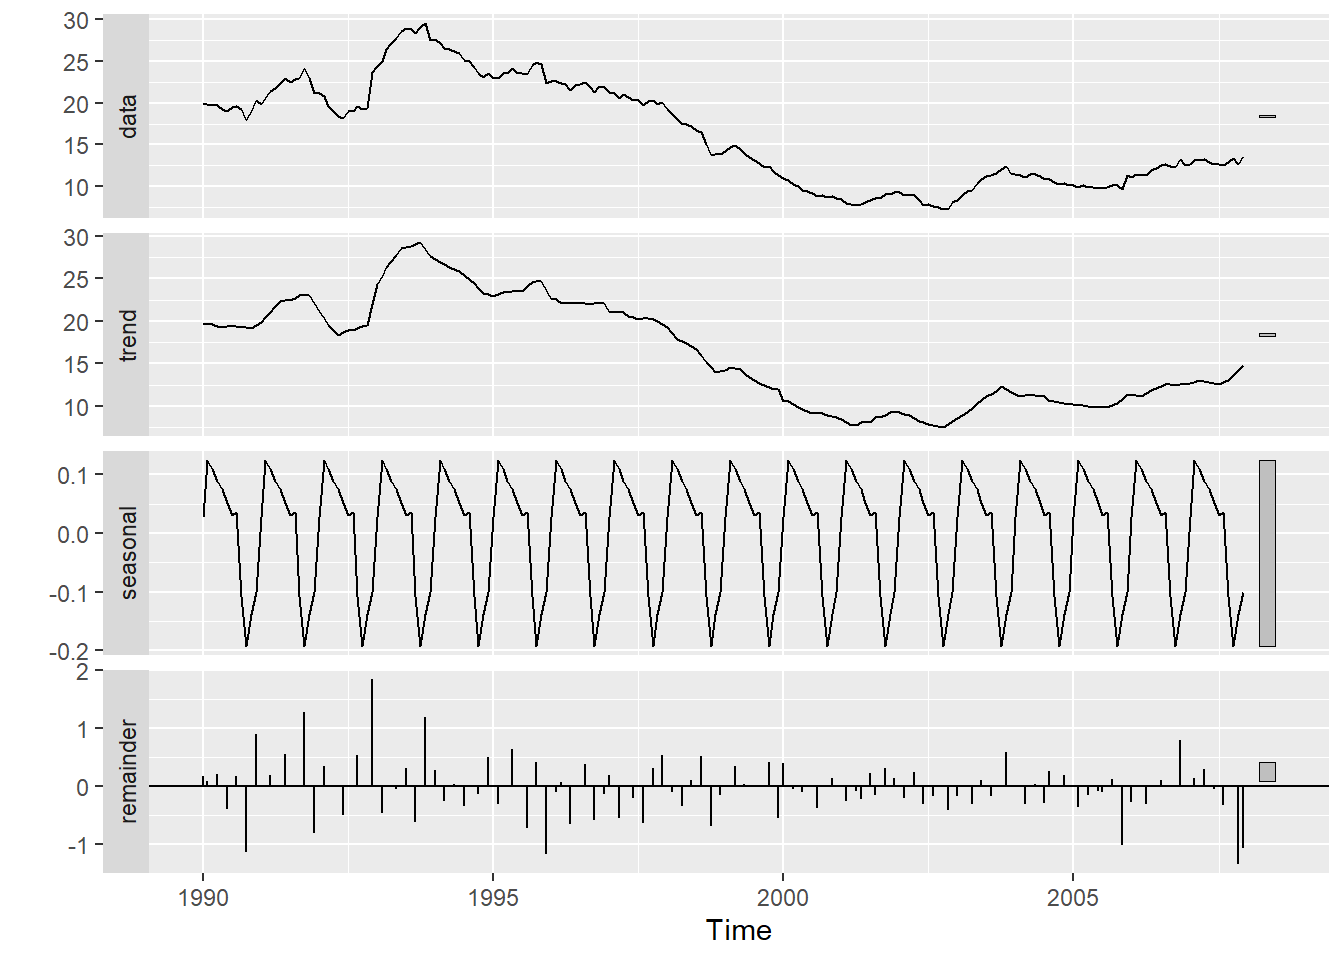
\includegraphics{final_analysis_files/figure-latex/unnamed-chunk-8-1.pdf}

\begin{Shaded}
\begin{Highlighting}[]
\NormalTok{g1 <-}\StringTok{ }\KeywordTok{ggplot}\NormalTok{(}\DataTypeTok{data=}\NormalTok{movies, }\KeywordTok{aes}\NormalTok{(}\DataTypeTok{x=}\NormalTok{audience_score)) }\OperatorTok{+}\StringTok{ }\KeywordTok{geom_density}\NormalTok{(}\KeywordTok{aes}\NormalTok{(}\DataTypeTok{color =}\NormalTok{ title_type), }\DataTypeTok{kernel =} \StringTok{"gaussian"}\NormalTok{)}
\NormalTok{g2 <-}\StringTok{ }\KeywordTok{ggplot}\NormalTok{(}\DataTypeTok{data=}\NormalTok{movies, }\KeywordTok{aes}\NormalTok{(}\DataTypeTok{x=}\NormalTok{critics_score)) }\OperatorTok{+}\StringTok{ }\KeywordTok{geom_density}\NormalTok{(}\KeywordTok{aes}\NormalTok{(}\DataTypeTok{color =}\NormalTok{ title_type), }\DataTypeTok{kernel =} \StringTok{"gaussian"}\NormalTok{)}
\NormalTok{g3 <-}\StringTok{ }\KeywordTok{ggplot}\NormalTok{(}\DataTypeTok{data=}\NormalTok{movies, }\KeywordTok{aes}\NormalTok{(}\DataTypeTok{x=}\NormalTok{imdb_rating)) }\OperatorTok{+}\StringTok{ }\KeywordTok{geom_density}\NormalTok{(}\KeywordTok{aes}\NormalTok{(}\DataTypeTok{color =}\NormalTok{ title_type), }\DataTypeTok{kernel =} \StringTok{"gaussian"}\NormalTok{)}

\KeywordTok{ggarrange}\NormalTok{(}
\NormalTok{    g1,}
\NormalTok{    g2,}
\NormalTok{    g3,}
    \DataTypeTok{ncol =} \DecValTok{3}\NormalTok{,}
    \DataTypeTok{nrow =} \DecValTok{1}\NormalTok{,}
    \DataTypeTok{widths =} \KeywordTok{c}\NormalTok{(}\DecValTok{200}\NormalTok{,}\DecValTok{200}\NormalTok{,}\DecValTok{400}\NormalTok{)}
\NormalTok{  )}
\end{Highlighting}
\end{Shaded}

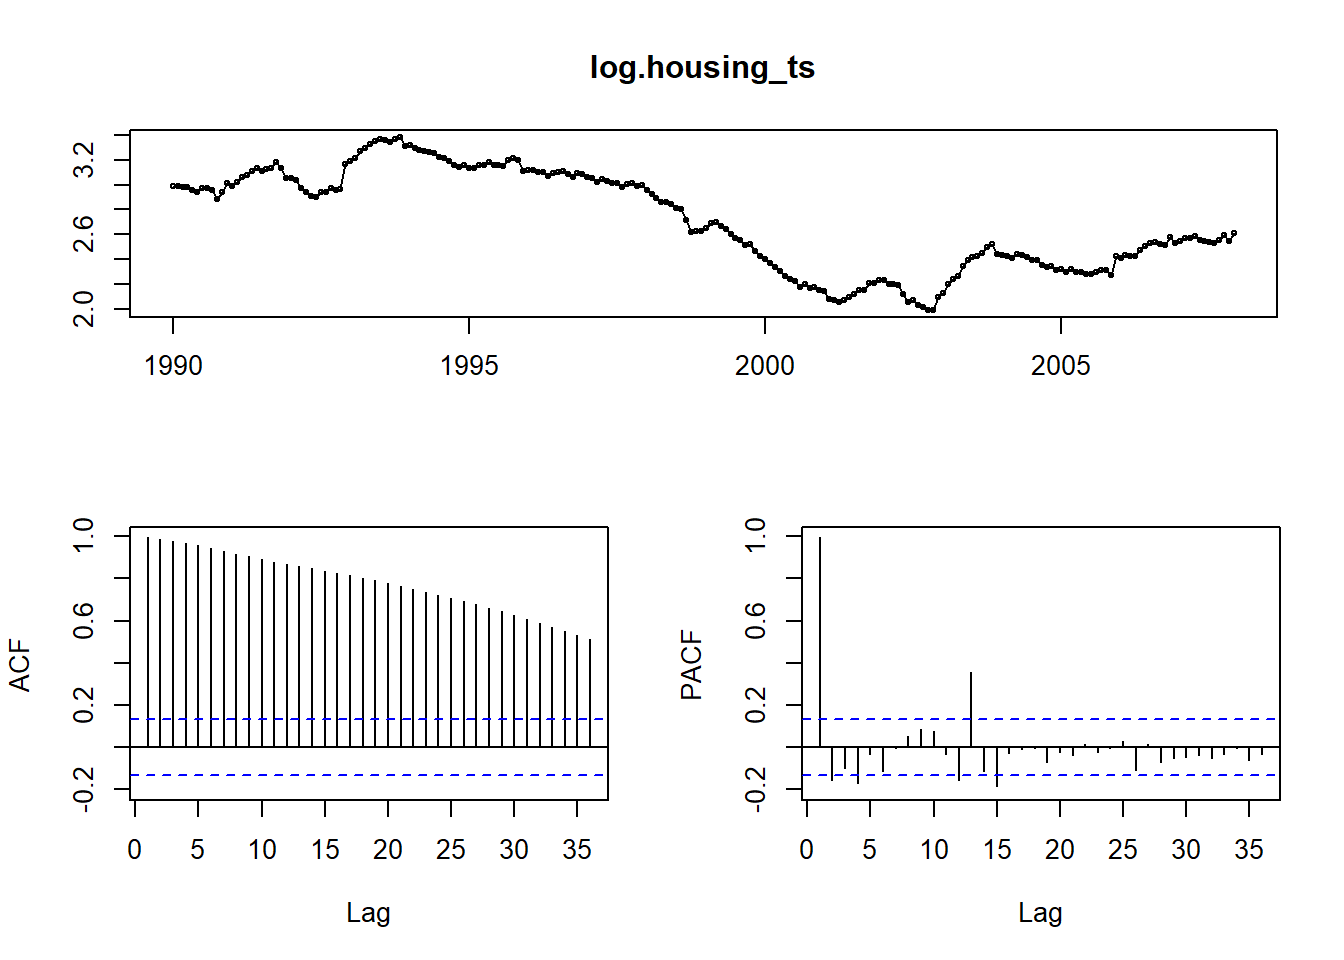
\includegraphics{final_analysis_files/figure-latex/unnamed-chunk-9-1.pdf}

\begin{Shaded}
\begin{Highlighting}[]
\KeywordTok{ggplot}\NormalTok{(}\DataTypeTok{data=}\NormalTok{movies, }\KeywordTok{aes}\NormalTok{(}\DataTypeTok{x =} \KeywordTok{reorder}\NormalTok{(genre, audience_score, median, }\DataTypeTok{order=}\OtherTok{TRUE}\NormalTok{), }\DataTypeTok{y =}\NormalTok{ audience_score, }\DataTypeTok{group =}\NormalTok{ genre, }\DataTypeTok{fill =}\NormalTok{ genre)) }\OperatorTok{+}\StringTok{ }\KeywordTok{geom_boxplot}\NormalTok{(}\DataTypeTok{alpha =} \FloatTok{.7}\NormalTok{) }\OperatorTok{+}\StringTok{ }\KeywordTok{geom_jitter}\NormalTok{(}\DataTypeTok{width =} \FloatTok{.05}\NormalTok{, }\DataTypeTok{alpha =} \FloatTok{.4}\NormalTok{) }\OperatorTok{+}\StringTok{ }\KeywordTok{guides}\NormalTok{(}\DataTypeTok{fill =} \StringTok{"none"}\NormalTok{) }\OperatorTok{+}\StringTok{ }\KeywordTok{theme_bw}\NormalTok{() }\OperatorTok{+}\StringTok{ }\KeywordTok{coord_flip}\NormalTok{()}
\end{Highlighting}
\end{Shaded}

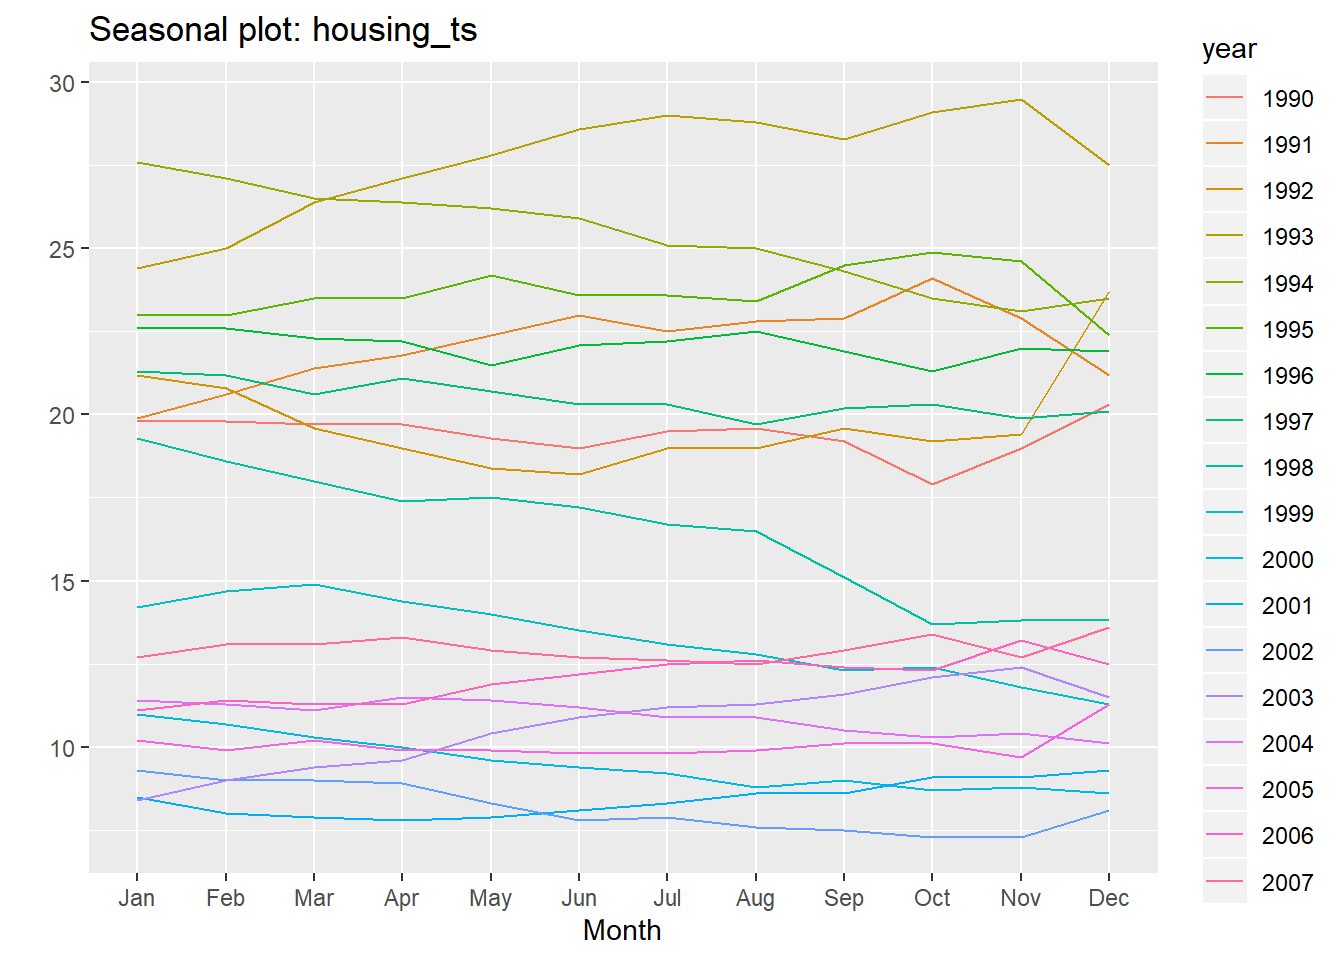
\includegraphics{final_analysis_files/figure-latex/unnamed-chunk-10-1.pdf}

\begin{Shaded}
\begin{Highlighting}[]
\KeywordTok{ggplot}\NormalTok{(}\DataTypeTok{data=}\NormalTok{movies, }\KeywordTok{aes}\NormalTok{(}\DataTypeTok{x =} \KeywordTok{reorder}\NormalTok{(genre, critics_score, median, }\DataTypeTok{order=}\OtherTok{TRUE}\NormalTok{), }\DataTypeTok{y =}\NormalTok{ critics_score, }\DataTypeTok{group =}\NormalTok{ genre, }\DataTypeTok{fill =}\NormalTok{ genre)) }\OperatorTok{+}\StringTok{ }\KeywordTok{geom_boxplot}\NormalTok{(}\DataTypeTok{alpha =} \FloatTok{.7}\NormalTok{) }\OperatorTok{+}\StringTok{ }\KeywordTok{geom_jitter}\NormalTok{(}\DataTypeTok{width =} \FloatTok{.05}\NormalTok{, }\DataTypeTok{alpha =} \FloatTok{.4}\NormalTok{) }\OperatorTok{+}\StringTok{ }\KeywordTok{guides}\NormalTok{(}\DataTypeTok{fill =} \StringTok{"none"}\NormalTok{) }\OperatorTok{+}\StringTok{ }\KeywordTok{theme_bw}\NormalTok{() }\OperatorTok{+}\StringTok{ }\KeywordTok{coord_flip}\NormalTok{()}
\end{Highlighting}
\end{Shaded}

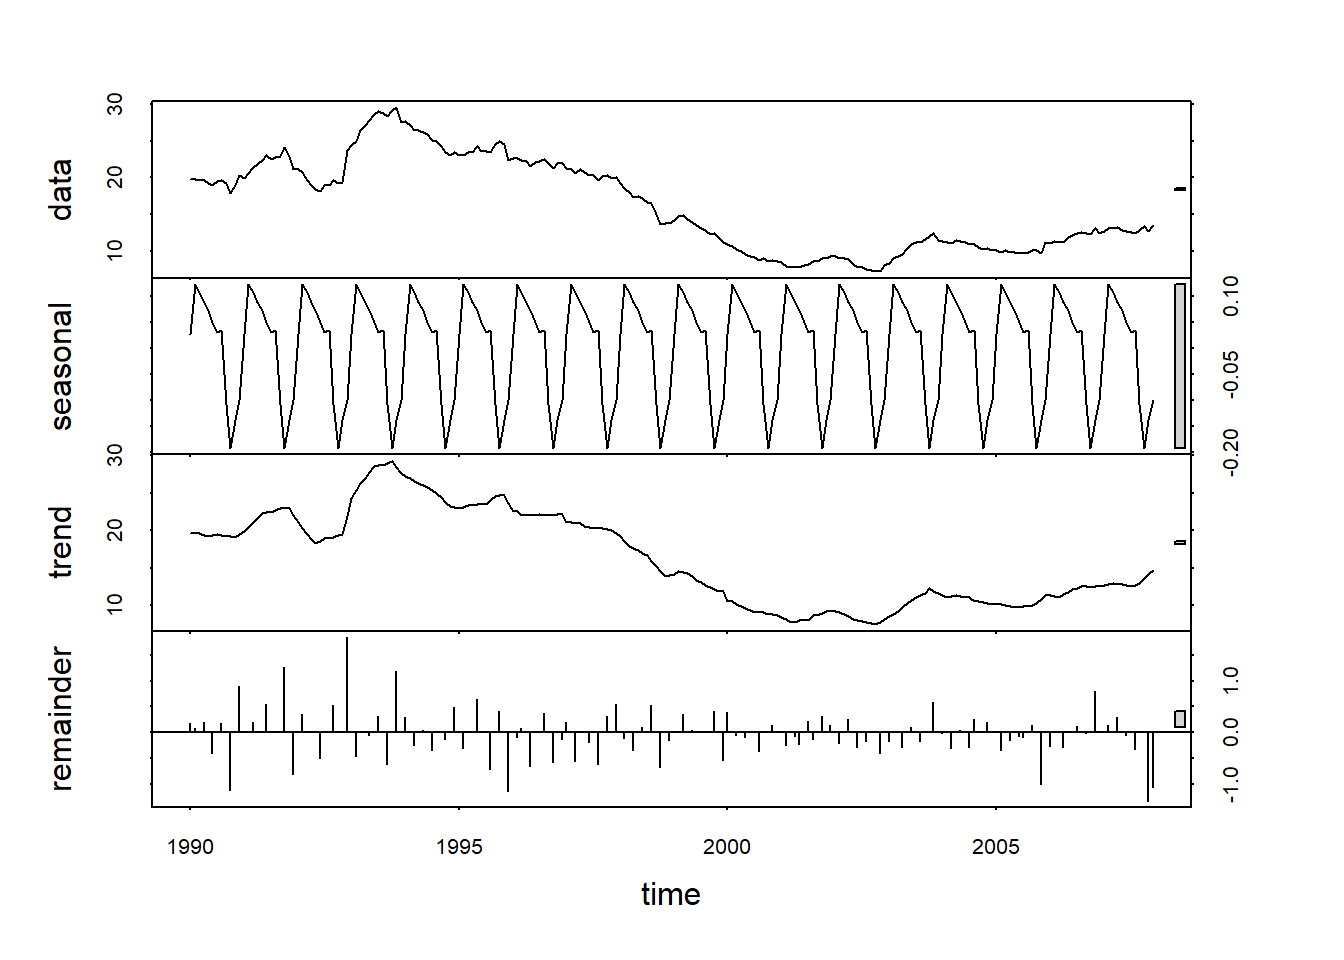
\includegraphics{final_analysis_files/figure-latex/unnamed-chunk-11-1.pdf}

\begin{Shaded}
\begin{Highlighting}[]
\KeywordTok{ggplot}\NormalTok{(}\DataTypeTok{data=}\NormalTok{movies, }\KeywordTok{aes}\NormalTok{(}\DataTypeTok{x =} \KeywordTok{reorder}\NormalTok{(genre, imdb_rating, median, }\DataTypeTok{order=}\OtherTok{TRUE}\NormalTok{), }\DataTypeTok{y =}\NormalTok{ imdb_rating, }\DataTypeTok{group =}\NormalTok{ genre, }\DataTypeTok{fill =}\NormalTok{ genre)) }\OperatorTok{+}\StringTok{ }\KeywordTok{geom_boxplot}\NormalTok{(}\DataTypeTok{alpha =} \FloatTok{.7}\NormalTok{) }\OperatorTok{+}\StringTok{ }\KeywordTok{geom_jitter}\NormalTok{(}\DataTypeTok{width =} \FloatTok{.05}\NormalTok{, }\DataTypeTok{alpha =} \FloatTok{.4}\NormalTok{) }\OperatorTok{+}\StringTok{ }\KeywordTok{guides}\NormalTok{(}\DataTypeTok{fill =} \StringTok{"none"}\NormalTok{) }\OperatorTok{+}\StringTok{ }\KeywordTok{theme_bw}\NormalTok{() }\OperatorTok{+}\StringTok{ }\KeywordTok{coord_flip}\NormalTok{()}
\end{Highlighting}
\end{Shaded}

\includegraphics{final_analysis_files/figure-latex/unnamed-chunk-12-1.pdf}

\hypertarget{comparing-different-scores-criticsaudienceimdb-1}{%
\subsection{2. Comparing different scores
(critics/audience/imdb)}\label{comparing-different-scores-criticsaudienceimdb-1}}

\hypertarget{is-there-any-difference-on-the-audiencecritics-score-by-genre}{%
\subsubsection{- Is there any difference on the audience/critics score
by
genre?}\label{is-there-any-difference-on-the-audiencecritics-score-by-genre}}

\hypertarget{is-there-any-difference-on-the-audiencecritics-score-by-mpaa-score}{%
\subsubsection{- Is there any difference on the audience/critics score
by MPAA
score?}\label{is-there-any-difference-on-the-audiencecritics-score-by-mpaa-score}}

\begin{Shaded}
\begin{Highlighting}[]
\NormalTok{score =}\StringTok{ }\KeywordTok{list}\NormalTok{();}

\NormalTok{score}\OperatorTok{$}\NormalTok{genre_score_agg =}\StringTok{ }\KeywordTok{list}\NormalTok{(}
  \StringTok{"critics"}\NormalTok{ =}\StringTok{ }\KeywordTok{aggregate}\NormalTok{(critics_score }\OperatorTok{~}\StringTok{ }\NormalTok{genre , movies, mean),}
  \StringTok{"audience"}\NormalTok{ =}\StringTok{ }\KeywordTok{aggregate}\NormalTok{(audience_score }\OperatorTok{~}\StringTok{ }\NormalTok{genre, movies, mean),}
  \StringTok{"imdb"}\NormalTok{ =}\StringTok{ }\KeywordTok{aggregate}\NormalTok{(imdb_rating }\OperatorTok{~}\StringTok{ }\NormalTok{genre, movies, mean)}
\NormalTok{)}


\NormalTok{score}\OperatorTok{$}\NormalTok{genre_metrics_grid =}\StringTok{ }\KeywordTok{expand.grid}\NormalTok{(}\DataTypeTok{year =}\KeywordTok{sort}\NormalTok{(}\KeywordTok{unique}\NormalTok{(movies}\OperatorTok{$}\NormalTok{genre)),}
                                       \DataTypeTok{metrics =} \KeywordTok{c}\NormalTok{(}\StringTok{"Critic"}\NormalTok{, }\StringTok{"Audience"}\NormalTok{, }\StringTok{"IMDB"}\NormalTok{))}

\NormalTok{score}\OperatorTok{$}\NormalTok{genre_metrics_grid}\OperatorTok{$}\NormalTok{genre_score_agg =}\KeywordTok{c}\NormalTok{(score}\OperatorTok{$}\NormalTok{genre_score_agg}\OperatorTok{$}\NormalTok{critics}\OperatorTok{$}\NormalTok{critics_score,}
\NormalTok{                                            score}\OperatorTok{$}\NormalTok{genre_score_agg}\OperatorTok{$}\NormalTok{audience}\OperatorTok{$}\NormalTok{audience_score, }
\NormalTok{                                            score}\OperatorTok{$}\NormalTok{genre_score_agg}\OperatorTok{$}\NormalTok{imdb}\OperatorTok{$}\NormalTok{imdb_rating)}

\NormalTok{score}\OperatorTok{$}\NormalTok{genre_metrics_grid}\OperatorTok{$}\NormalTok{genre_score_agg_rescaled =}\StringTok{ }
\StringTok{  }\KeywordTok{c}\NormalTok{(}
    \KeywordTok{rescale}\NormalTok{(score}\OperatorTok{$}\NormalTok{genre_score_agg}\OperatorTok{$}\NormalTok{critics}\OperatorTok{$}\NormalTok{critics_score, }\DataTypeTok{from=}\NormalTok{(}\KeywordTok{c}\NormalTok{(}\DecValTok{1}\NormalTok{,}\DecValTok{100}\NormalTok{))), }
    \KeywordTok{rescale}\NormalTok{(score}\OperatorTok{$}\NormalTok{genre_score_agg}\OperatorTok{$}\NormalTok{audience}\OperatorTok{$}\NormalTok{audience_score, }\DataTypeTok{from=}\NormalTok{(}\KeywordTok{c}\NormalTok{(}\DecValTok{1}\NormalTok{,}\DecValTok{100}\NormalTok{))), }
    \KeywordTok{rescale}\NormalTok{(score}\OperatorTok{$}\NormalTok{genre_score_agg}\OperatorTok{$}\NormalTok{imdb}\OperatorTok{$}\NormalTok{imdb_rating, }\DataTypeTok{from=}\NormalTok{(}\KeywordTok{c}\NormalTok{(}\DecValTok{1}\NormalTok{,}\DecValTok{10}\NormalTok{))))}

\KeywordTok{ggplot}\NormalTok{(score}\OperatorTok{$}\NormalTok{genre_metrics_grid)}\OperatorTok{+}
\StringTok{  }\KeywordTok{geom_tile}\NormalTok{(}\KeywordTok{aes}\NormalTok{(}\DataTypeTok{x=}\NormalTok{metrics, }\DataTypeTok{y=}\NormalTok{year,}\DataTypeTok{fill=}\NormalTok{genre_score_agg_rescaled))}\OperatorTok{+}
\StringTok{  }\KeywordTok{scale_fill_distiller}\NormalTok{( }\DataTypeTok{limits=}\KeywordTok{c}\NormalTok{(}\DecValTok{0}\NormalTok{,}\DecValTok{1}\NormalTok{), }\DataTypeTok{palette =} \StringTok{"PuOr"}\NormalTok{) }\OperatorTok{+}
\StringTok{  }\KeywordTok{labs}\NormalTok{(}\DataTypeTok{title =} \StringTok{"Comparision of scores across genres (Heatmap)"}\NormalTok{, }\DataTypeTok{x =} \StringTok{""}\NormalTok{, }\DataTypeTok{y=}\StringTok{""}\NormalTok{, }\DataTypeTok{fill=}\StringTok{""}\NormalTok{)}\OperatorTok{+}
\StringTok{  }\KeywordTok{theme}\NormalTok{(}\DataTypeTok{plot.title =} \KeywordTok{element_text}\NormalTok{(}\DataTypeTok{hjust =} \FloatTok{0.5}\NormalTok{))}
\end{Highlighting}
\end{Shaded}

\includegraphics{final_analysis_files/figure-latex/unnamed-chunk-13-1.pdf}

To compare the three different score types: Critic, Audience and IMDB to
be comaral they must be rescaled as while Critic and Audience are of the
range 1-100, IMDB is 1-10. After rescaling, to the range 0-1, a visual
comparison of the different groups can be seen by arranging them on a
heatmap.

The most striking feature is the lack of high scores for most genres,
except for Documentary and Musical \& Performing Arts. From the three
groups Critics seem to be the most negative in their scoring, while
Audience and IMDB to be more aligned. This clearly seen in Action \&
Adventure genre where Critics have a far lower score than the other two
groups. This may be due to Critics having a different criteria on what
constitutes a ``good'' movie but without details on the required metrics
this is only speculation. Conversely though IMBD scores are most
unaligned with the other groups for the two highest scoring genres, the
reasoning for this can not be determined from the data available.

\begin{Shaded}
\begin{Highlighting}[]
\NormalTok{mean_score <-}
\StringTok{  }\KeywordTok{data.frame}\NormalTok{(}
    \StringTok{"Score"}\NormalTok{ =}\StringTok{ }\KeywordTok{c}\NormalTok{(}
      \KeywordTok{mean}\NormalTok{(movies}\OperatorTok{$}\NormalTok{imdb_rating)}\OperatorTok{*}\DecValTok{10}\NormalTok{,}
      \KeywordTok{mean}\NormalTok{(movies}\OperatorTok{$}\NormalTok{audience_score),}
      \KeywordTok{mean}\NormalTok{(movies}\OperatorTok{$}\NormalTok{critics_score)}
\NormalTok{    ),}
    \StringTok{"Source"}\NormalTok{ =}\StringTok{ }\KeywordTok{c}\NormalTok{(}\StringTok{"IMDB"}\NormalTok{, }\StringTok{"Audience"}\NormalTok{, }\StringTok{"Critics"}\NormalTok{)}
\NormalTok{  )}

\NormalTok{plot_all <-}\StringTok{ }\KeywordTok{ggplot}\NormalTok{(mean_score, }\KeywordTok{aes}\NormalTok{(Score, Source)) }\OperatorTok{+}
\StringTok{  }\KeywordTok{geom_segment}\NormalTok{(}\KeywordTok{aes}\NormalTok{(}\DataTypeTok{x =} \DecValTok{0}\NormalTok{, }\DataTypeTok{y =}\NormalTok{ Source, }\DataTypeTok{xend =}\NormalTok{ Score, }\DataTypeTok{yend =}\NormalTok{ Source,}\DataTypeTok{colour=}\NormalTok{Source) ) }\OperatorTok{+}
\StringTok{  }\KeywordTok{geom_point}\NormalTok{(}\KeywordTok{aes}\NormalTok{(  }\DataTypeTok{colour=}\NormalTok{Source) ) }\OperatorTok{+}\StringTok{ }\KeywordTok{xlim}\NormalTok{(}\DecValTok{0}\NormalTok{, }\DecValTok{88}\NormalTok{) }\OperatorTok{+}\StringTok{ }\KeywordTok{theme}\NormalTok{(}\DataTypeTok{legend.position =} \StringTok{"none"}\NormalTok{,}\DataTypeTok{axis.title.x =} \KeywordTok{element_blank}\NormalTok{(), }\DataTypeTok{axis.text.y =} \KeywordTok{element_blank}\NormalTok{()) }\OperatorTok{+}\StringTok{ }\KeywordTok{ggtitle}\NormalTok{(}\StringTok{"All genres"}\NormalTok{)}

\CommentTok{#Action and adventure}
\NormalTok{action_adventure <-}\StringTok{ }\KeywordTok{subset}\NormalTok{(movies, genre }\OperatorTok{==}\StringTok{ "Action & Adventure"}\NormalTok{)}
\NormalTok{mean_score <-}
\StringTok{  }\KeywordTok{data.frame}\NormalTok{(}
    \StringTok{"Score"}\NormalTok{ =}\StringTok{ }\KeywordTok{c}\NormalTok{(}
      \KeywordTok{mean}\NormalTok{(action_adventure}\OperatorTok{$}\NormalTok{imdb_rating)}\OperatorTok{*}\DecValTok{10}\NormalTok{,}
      \KeywordTok{mean}\NormalTok{(action_adventure}\OperatorTok{$}\NormalTok{audience_score),}
      \KeywordTok{mean}\NormalTok{(action_adventure}\OperatorTok{$}\NormalTok{critics_score)}
\NormalTok{    ),}
    \StringTok{"Source"}\NormalTok{ =}\StringTok{ }\KeywordTok{c}\NormalTok{(}\StringTok{"IMDB"}\NormalTok{, }\StringTok{"Audience"}\NormalTok{, }\StringTok{"Critics"}\NormalTok{)}
\NormalTok{  )}

\NormalTok{plot_action <-}\StringTok{ }\KeywordTok{ggplot}\NormalTok{(mean_score, }\KeywordTok{aes}\NormalTok{(Score, Source)) }\OperatorTok{+}
\StringTok{  }\KeywordTok{geom_segment}\NormalTok{(}\KeywordTok{aes}\NormalTok{(}\DataTypeTok{x =} \DecValTok{0}\NormalTok{, }\DataTypeTok{y =}\NormalTok{ Source, }\DataTypeTok{xend =}\NormalTok{ Score, }\DataTypeTok{yend =}\NormalTok{ Source,}\DataTypeTok{colour=}\NormalTok{Source) ) }\OperatorTok{+}
\StringTok{  }\KeywordTok{geom_point}\NormalTok{(}\KeywordTok{aes}\NormalTok{(  }\DataTypeTok{colour=}\NormalTok{Source) ) }\OperatorTok{+}\StringTok{ }\KeywordTok{xlim}\NormalTok{(}\DecValTok{0}\NormalTok{, }\DecValTok{88}\NormalTok{) }\OperatorTok{+}\StringTok{ }\KeywordTok{theme}\NormalTok{(}\DataTypeTok{legend.position =} \StringTok{"none"}\NormalTok{,}\DataTypeTok{axis.title.x =} \KeywordTok{element_blank}\NormalTok{(),}\DataTypeTok{axis.title.y =} \KeywordTok{element_blank}\NormalTok{(),}\DataTypeTok{axis.text.y =} \KeywordTok{element_blank}\NormalTok{()) }\OperatorTok{+}\StringTok{ }\KeywordTok{ggtitle}\NormalTok{(}\StringTok{"Action & Adventure"}\NormalTok{)}

\CommentTok{#Animation}
\NormalTok{animation <-}\StringTok{ }\KeywordTok{subset}\NormalTok{(movies, genre }\OperatorTok{==}\StringTok{ "Animation"}\NormalTok{)}
\NormalTok{mean_score <-}
\StringTok{  }\KeywordTok{data.frame}\NormalTok{(}
    \StringTok{"Score"}\NormalTok{ =}\StringTok{ }\KeywordTok{c}\NormalTok{(}
      \KeywordTok{mean}\NormalTok{(animation}\OperatorTok{$}\NormalTok{imdb_rating)}\OperatorTok{*}\DecValTok{10}\NormalTok{,}
      \KeywordTok{mean}\NormalTok{(animation}\OperatorTok{$}\NormalTok{audience_score),}
      \KeywordTok{mean}\NormalTok{(animation}\OperatorTok{$}\NormalTok{critics_score)}
\NormalTok{    ),}
    \StringTok{"Source"}\NormalTok{ =}\StringTok{ }\KeywordTok{c}\NormalTok{(}\StringTok{"IMDB"}\NormalTok{, }\StringTok{"Audience"}\NormalTok{, }\StringTok{"Critics"}\NormalTok{)}
\NormalTok{  )}

\NormalTok{plot_animation <-}\StringTok{ }\KeywordTok{ggplot}\NormalTok{(mean_score, }\KeywordTok{aes}\NormalTok{(Score, Source)) }\OperatorTok{+}
\StringTok{  }\KeywordTok{geom_segment}\NormalTok{(}\KeywordTok{aes}\NormalTok{(}\DataTypeTok{x =} \DecValTok{0}\NormalTok{, }\DataTypeTok{y =}\NormalTok{ Source, }\DataTypeTok{xend =}\NormalTok{ Score, }\DataTypeTok{yend =}\NormalTok{ Source,}\DataTypeTok{colour=}\NormalTok{Source) ) }\OperatorTok{+}
\StringTok{  }\KeywordTok{geom_point}\NormalTok{(}\KeywordTok{aes}\NormalTok{(  }\DataTypeTok{colour=}\NormalTok{Source) ) }\OperatorTok{+}\StringTok{ }\KeywordTok{xlim}\NormalTok{(}\DecValTok{0}\NormalTok{, }\DecValTok{88}\NormalTok{) }\OperatorTok{+}\StringTok{ }\KeywordTok{theme}\NormalTok{(}\DataTypeTok{legend.position =} \StringTok{"none"}\NormalTok{,}\DataTypeTok{axis.title.x =} \KeywordTok{element_blank}\NormalTok{(),}\DataTypeTok{axis.title.y =} \KeywordTok{element_blank}\NormalTok{(),}\DataTypeTok{axis.text.y =} \KeywordTok{element_blank}\NormalTok{()) }\OperatorTok{+}\StringTok{ }\KeywordTok{ggtitle}\NormalTok{(}\StringTok{"Animation"}\NormalTok{)}

\CommentTok{#Art House & International}
\NormalTok{art_house <-}\StringTok{ }\KeywordTok{subset}\NormalTok{(movies, genre }\OperatorTok{==}\StringTok{ "Art House & International"}\NormalTok{)}

\NormalTok{mean_score <-}
\StringTok{  }\KeywordTok{data.frame}\NormalTok{(}
    \StringTok{"Score"}\NormalTok{ =}\StringTok{ }\KeywordTok{c}\NormalTok{(}
      \KeywordTok{mean}\NormalTok{(art_house}\OperatorTok{$}\NormalTok{imdb_rating)}\OperatorTok{*}\DecValTok{10}\NormalTok{,}
      \KeywordTok{mean}\NormalTok{(art_house}\OperatorTok{$}\NormalTok{audience_score),}
      \KeywordTok{mean}\NormalTok{(art_house}\OperatorTok{$}\NormalTok{critics_score)}
\NormalTok{    ),}
    \StringTok{"Source"}\NormalTok{ =}\StringTok{ }\KeywordTok{c}\NormalTok{(}\StringTok{"IMDB"}\NormalTok{, }\StringTok{"Audience"}\NormalTok{, }\StringTok{"Critics"}\NormalTok{)}
\NormalTok{  )}

\NormalTok{plot_art_house <-}\StringTok{ }\KeywordTok{ggplot}\NormalTok{(mean_score, }\KeywordTok{aes}\NormalTok{(Score, Source)) }\OperatorTok{+}
\StringTok{  }\KeywordTok{geom_segment}\NormalTok{(}\KeywordTok{aes}\NormalTok{(}\DataTypeTok{x =} \DecValTok{0}\NormalTok{, }\DataTypeTok{y =}\NormalTok{ Source, }\DataTypeTok{xend =}\NormalTok{ Score, }\DataTypeTok{yend =}\NormalTok{ Source,}\DataTypeTok{colour=}\NormalTok{Source) ) }\OperatorTok{+}
\StringTok{  }\KeywordTok{geom_point}\NormalTok{(}\KeywordTok{aes}\NormalTok{(  }\DataTypeTok{colour=}\NormalTok{Source) ) }\OperatorTok{+}\StringTok{ }\KeywordTok{xlim}\NormalTok{(}\DecValTok{0}\NormalTok{, }\DecValTok{88}\NormalTok{) }\OperatorTok{+}\StringTok{ }\KeywordTok{theme}\NormalTok{(}\DataTypeTok{legend.position =} \StringTok{"none"}\NormalTok{,}\DataTypeTok{axis.title.x =} \KeywordTok{element_blank}\NormalTok{(),}\DataTypeTok{axis.text.y =} \KeywordTok{element_blank}\NormalTok{()) }\OperatorTok{+}\StringTok{ }\KeywordTok{ggtitle}\NormalTok{(}\StringTok{"Art House & International"}\NormalTok{)}

\CommentTok{#Comedy}
\NormalTok{comedy <-}\StringTok{ }\KeywordTok{subset}\NormalTok{(movies, genre }\OperatorTok{==}\StringTok{ "Comedy"}\NormalTok{)}

\NormalTok{mean_score <-}
\StringTok{  }\KeywordTok{data.frame}\NormalTok{(}
    \StringTok{"Score"}\NormalTok{ =}\StringTok{ }\KeywordTok{c}\NormalTok{(}
      \KeywordTok{mean}\NormalTok{(comedy}\OperatorTok{$}\NormalTok{imdb_rating)}\OperatorTok{*}\DecValTok{10}\NormalTok{,}
      \KeywordTok{mean}\NormalTok{(comedy}\OperatorTok{$}\NormalTok{audience_score),}
      \KeywordTok{mean}\NormalTok{(comedy}\OperatorTok{$}\NormalTok{critics_score)}
\NormalTok{    ),}
    \StringTok{"Source"}\NormalTok{ =}\StringTok{ }\KeywordTok{c}\NormalTok{(}\StringTok{"IMDB"}\NormalTok{, }\StringTok{"Audience"}\NormalTok{, }\StringTok{"Critics"}\NormalTok{)}
\NormalTok{  )}
\NormalTok{plot_comedy <-}\KeywordTok{ggplot}\NormalTok{(mean_score, }\KeywordTok{aes}\NormalTok{(Score, Source)) }\OperatorTok{+}
\StringTok{  }\KeywordTok{geom_segment}\NormalTok{(}\KeywordTok{aes}\NormalTok{(}\DataTypeTok{x =} \DecValTok{0}\NormalTok{, }\DataTypeTok{y =}\NormalTok{ Source, }\DataTypeTok{xend =}\NormalTok{ Score, }\DataTypeTok{yend =}\NormalTok{ Source,}\DataTypeTok{colour=}\NormalTok{Source) ) }\OperatorTok{+}
\StringTok{  }\KeywordTok{geom_point}\NormalTok{(}\KeywordTok{aes}\NormalTok{(  }\DataTypeTok{colour=}\NormalTok{Source) ) }\OperatorTok{+}\StringTok{ }\KeywordTok{xlim}\NormalTok{(}\DecValTok{0}\NormalTok{, }\DecValTok{88}\NormalTok{) }\OperatorTok{+}\StringTok{ }\KeywordTok{theme}\NormalTok{(}\DataTypeTok{legend.position =} \StringTok{"none"}\NormalTok{,}\DataTypeTok{axis.title.x =} \KeywordTok{element_blank}\NormalTok{(),}\DataTypeTok{axis.title.y =} \KeywordTok{element_blank}\NormalTok{(),}\DataTypeTok{axis.text.y =} \KeywordTok{element_blank}\NormalTok{()) }\OperatorTok{+}\StringTok{ }\KeywordTok{ggtitle}\NormalTok{(}\StringTok{"Comedy"}\NormalTok{)}

\CommentTok{#Documentary}
\NormalTok{documentary <-}\StringTok{ }\KeywordTok{subset}\NormalTok{(movies, genre }\OperatorTok{==}\StringTok{ "Documentary"}\NormalTok{)}

\NormalTok{mean_score <-}
\StringTok{  }\KeywordTok{data.frame}\NormalTok{(}
    \StringTok{"Score"}\NormalTok{ =}\StringTok{ }\KeywordTok{c}\NormalTok{(}
      \KeywordTok{mean}\NormalTok{(documentary}\OperatorTok{$}\NormalTok{imdb_rating)}\OperatorTok{*}\DecValTok{10}\NormalTok{,}
      \KeywordTok{mean}\NormalTok{(documentary}\OperatorTok{$}\NormalTok{audience_score),}
      \KeywordTok{mean}\NormalTok{(documentary}\OperatorTok{$}\NormalTok{critics_score)}
\NormalTok{    ),}
    \StringTok{"Source"}\NormalTok{ =}\StringTok{ }\KeywordTok{c}\NormalTok{(}\StringTok{"IMDB"}\NormalTok{, }\StringTok{"Audience"}\NormalTok{, }\StringTok{"Critics"}\NormalTok{)}
\NormalTok{  )}

\NormalTok{plot_documentary <-}\StringTok{ }\KeywordTok{ggplot}\NormalTok{(mean_score, }\KeywordTok{aes}\NormalTok{(Score, Source)) }\OperatorTok{+}
\StringTok{  }\KeywordTok{geom_segment}\NormalTok{(}\KeywordTok{aes}\NormalTok{(}\DataTypeTok{x =} \DecValTok{0}\NormalTok{, }\DataTypeTok{y =}\NormalTok{ Source, }\DataTypeTok{xend =}\NormalTok{ Score, }\DataTypeTok{yend =}\NormalTok{ Source,}\DataTypeTok{colour=}\NormalTok{Source) ) }\OperatorTok{+}
\StringTok{  }\KeywordTok{geom_point}\NormalTok{(}\KeywordTok{aes}\NormalTok{(  }\DataTypeTok{colour=}\NormalTok{Source) ) }\OperatorTok{+}\StringTok{ }\KeywordTok{xlim}\NormalTok{(}\DecValTok{0}\NormalTok{, }\DecValTok{88}\NormalTok{) }\OperatorTok{+}\StringTok{ }\KeywordTok{theme}\NormalTok{(}\DataTypeTok{legend.position =} \StringTok{"none"}\NormalTok{,}\DataTypeTok{axis.title.x =} \KeywordTok{element_blank}\NormalTok{(),}\DataTypeTok{axis.title.y =} \KeywordTok{element_blank}\NormalTok{(),}\DataTypeTok{axis.text.y =} \KeywordTok{element_blank}\NormalTok{()) }\OperatorTok{+}\StringTok{ }\KeywordTok{ggtitle}\NormalTok{(}\StringTok{"Documentary"}\NormalTok{)}

\CommentTok{#Drama}
\NormalTok{drama <-}\StringTok{ }\KeywordTok{subset}\NormalTok{(movies, genre }\OperatorTok{==}\StringTok{ "Drama"}\NormalTok{)}

\NormalTok{mean_score <-}
\StringTok{  }\KeywordTok{data.frame}\NormalTok{(}
    \StringTok{"Score"}\NormalTok{ =}\StringTok{ }\KeywordTok{c}\NormalTok{(}
      \KeywordTok{mean}\NormalTok{(drama}\OperatorTok{$}\NormalTok{imdb_rating)}\OperatorTok{*}\DecValTok{10}\NormalTok{,}
      \KeywordTok{mean}\NormalTok{(drama}\OperatorTok{$}\NormalTok{audience_score),}
      \KeywordTok{mean}\NormalTok{(drama}\OperatorTok{$}\NormalTok{critics_score)}
\NormalTok{    ),}
    \StringTok{"Source"}\NormalTok{ =}\StringTok{ }\KeywordTok{c}\NormalTok{(}\StringTok{"IMDB"}\NormalTok{, }\StringTok{"Audience"}\NormalTok{, }\StringTok{"Critics"}\NormalTok{)}
\NormalTok{  )}

\NormalTok{plot_drama <-}\StringTok{ }\KeywordTok{ggplot}\NormalTok{(mean_score, }\KeywordTok{aes}\NormalTok{(Score, Source)) }\OperatorTok{+}
\StringTok{  }\KeywordTok{geom_segment}\NormalTok{(}\KeywordTok{aes}\NormalTok{(}\DataTypeTok{x =} \DecValTok{0}\NormalTok{, }\DataTypeTok{y =}\NormalTok{ Source, }\DataTypeTok{xend =}\NormalTok{ Score, }\DataTypeTok{yend =}\NormalTok{ Source,}\DataTypeTok{colour=}\NormalTok{Source) ) }\OperatorTok{+}
\StringTok{  }\KeywordTok{geom_point}\NormalTok{(}\KeywordTok{aes}\NormalTok{(  }\DataTypeTok{colour=}\NormalTok{Source) ) }\OperatorTok{+}\StringTok{ }\KeywordTok{xlim}\NormalTok{(}\DecValTok{0}\NormalTok{, }\DecValTok{88}\NormalTok{) }\OperatorTok{+}\StringTok{ }\KeywordTok{theme}\NormalTok{(}\DataTypeTok{legend.position =} \StringTok{"none"}\NormalTok{,}\DataTypeTok{axis.title.x =} \KeywordTok{element_blank}\NormalTok{(),}\DataTypeTok{axis.text.y =} \KeywordTok{element_blank}\NormalTok{()) }\OperatorTok{+}\StringTok{ }\KeywordTok{ggtitle}\NormalTok{(}\StringTok{"Drama"}\NormalTok{)}

\CommentTok{#Horror}
\NormalTok{horror <-}\StringTok{ }\KeywordTok{subset}\NormalTok{(movies, genre }\OperatorTok{==}\StringTok{ "Horror"}\NormalTok{)}

\NormalTok{mean_score <-}
\StringTok{  }\KeywordTok{data.frame}\NormalTok{(}
    \StringTok{"Score"}\NormalTok{ =}\StringTok{ }\KeywordTok{c}\NormalTok{(}
      \KeywordTok{mean}\NormalTok{(horror}\OperatorTok{$}\NormalTok{imdb_rating)}\OperatorTok{*}\DecValTok{10}\NormalTok{,}
      \KeywordTok{mean}\NormalTok{(horror}\OperatorTok{$}\NormalTok{audience_score),}
      \KeywordTok{mean}\NormalTok{(horror}\OperatorTok{$}\NormalTok{critics_score)}
\NormalTok{    ),}
    \StringTok{"Source"}\NormalTok{ =}\StringTok{ }\KeywordTok{c}\NormalTok{(}\StringTok{"IMDB"}\NormalTok{, }\StringTok{"Audience"}\NormalTok{, }\StringTok{"Critics"}\NormalTok{)}
\NormalTok{  )}

\NormalTok{plot_horror <-}\StringTok{ }\KeywordTok{ggplot}\NormalTok{(mean_score, }\KeywordTok{aes}\NormalTok{(Score, Source)) }\OperatorTok{+}
\StringTok{  }\KeywordTok{geom_segment}\NormalTok{(}\KeywordTok{aes}\NormalTok{(}\DataTypeTok{x =} \DecValTok{0}\NormalTok{, }\DataTypeTok{y =}\NormalTok{ Source, }\DataTypeTok{xend =}\NormalTok{ Score, }\DataTypeTok{yend =}\NormalTok{ Source,}\DataTypeTok{colour=}\NormalTok{Source) ) }\OperatorTok{+}
\StringTok{  }\KeywordTok{geom_point}\NormalTok{(}\KeywordTok{aes}\NormalTok{(  }\DataTypeTok{colour=}\NormalTok{Source) ) }\OperatorTok{+}\StringTok{ }\KeywordTok{xlim}\NormalTok{(}\DecValTok{0}\NormalTok{, }\DecValTok{88}\NormalTok{) }\OperatorTok{+}\StringTok{ }\KeywordTok{theme}\NormalTok{(}\DataTypeTok{legend.position =} \StringTok{"none"}\NormalTok{,}\DataTypeTok{axis.title.x =} \KeywordTok{element_blank}\NormalTok{(),}\DataTypeTok{axis.title.y =} \KeywordTok{element_blank}\NormalTok{(),}\DataTypeTok{axis.text.y =} \KeywordTok{element_blank}\NormalTok{()) }\OperatorTok{+}\StringTok{ }\KeywordTok{ggtitle}\NormalTok{(}\StringTok{"Horror"}\NormalTok{)}

\CommentTok{#Musical & Performing Arts}
\NormalTok{musical <-}\StringTok{ }\KeywordTok{subset}\NormalTok{(movies, genre }\OperatorTok{==}\StringTok{ "Musical & Performing Arts"}\NormalTok{)}

\NormalTok{mean_score <-}
\StringTok{  }\KeywordTok{data.frame}\NormalTok{(}
    \StringTok{"Score"}\NormalTok{ =}\StringTok{ }\KeywordTok{c}\NormalTok{(}
      \KeywordTok{mean}\NormalTok{(musical}\OperatorTok{$}\NormalTok{imdb_rating)}\OperatorTok{*}\DecValTok{10}\NormalTok{,}
      \KeywordTok{mean}\NormalTok{(musical}\OperatorTok{$}\NormalTok{audience_score),}
      \KeywordTok{mean}\NormalTok{(musical}\OperatorTok{$}\NormalTok{critics_score)}
\NormalTok{    ),}
    \StringTok{"Source"}\NormalTok{ =}\StringTok{ }\KeywordTok{c}\NormalTok{(}\StringTok{"IMDB"}\NormalTok{, }\StringTok{"Audience"}\NormalTok{, }\StringTok{"Critics"}\NormalTok{)}
\NormalTok{  )}

\NormalTok{plot_musical <-}\StringTok{ }\KeywordTok{ggplot}\NormalTok{(mean_score, }\KeywordTok{aes}\NormalTok{(Score, Source)) }\OperatorTok{+}
\StringTok{  }\KeywordTok{geom_segment}\NormalTok{(}\KeywordTok{aes}\NormalTok{(}\DataTypeTok{x =} \DecValTok{0}\NormalTok{, }\DataTypeTok{y =}\NormalTok{ Source, }\DataTypeTok{xend =}\NormalTok{ Score, }\DataTypeTok{yend =}\NormalTok{ Source,}\DataTypeTok{colour=}\NormalTok{Source) ) }\OperatorTok{+}
\StringTok{  }\KeywordTok{geom_point}\NormalTok{(}\KeywordTok{aes}\NormalTok{(  }\DataTypeTok{colour=}\NormalTok{Source) ) }\OperatorTok{+}\StringTok{ }\KeywordTok{xlim}\NormalTok{(}\DecValTok{0}\NormalTok{, }\DecValTok{88}\NormalTok{) }\OperatorTok{+}\StringTok{ }\KeywordTok{theme}\NormalTok{(}\DataTypeTok{legend.position =} \StringTok{"none"}\NormalTok{,}\DataTypeTok{axis.text.y =} \KeywordTok{element_blank}\NormalTok{()) }\OperatorTok{+}\StringTok{ }\KeywordTok{ggtitle}\NormalTok{(}\StringTok{"Musical & Performing Arts"}\NormalTok{)}

\CommentTok{#Mystery & Suspense}
\NormalTok{mistery <-}\StringTok{ }\KeywordTok{subset}\NormalTok{(movies, genre }\OperatorTok{==}\StringTok{ "Mystery & Suspense"}\NormalTok{)}
\NormalTok{mean_score <-}
\StringTok{  }\KeywordTok{data.frame}\NormalTok{(}
    \StringTok{"Score"}\NormalTok{ =}\StringTok{ }\KeywordTok{c}\NormalTok{(}
      \KeywordTok{mean}\NormalTok{(mistery}\OperatorTok{$}\NormalTok{imdb_rating)}\OperatorTok{*}\DecValTok{10}\NormalTok{,}
      \KeywordTok{mean}\NormalTok{(mistery}\OperatorTok{$}\NormalTok{audience_score),}
      \KeywordTok{mean}\NormalTok{(mistery}\OperatorTok{$}\NormalTok{critics_score)}
\NormalTok{    ),}
    \StringTok{"Source"}\NormalTok{ =}\StringTok{ }\KeywordTok{c}\NormalTok{(}\StringTok{"IMDB"}\NormalTok{, }\StringTok{"Audience"}\NormalTok{, }\StringTok{"Critics"}\NormalTok{)}
\NormalTok{  )}

\NormalTok{plot_mistery <-}\StringTok{ }\KeywordTok{ggplot}\NormalTok{(mean_score, }\KeywordTok{aes}\NormalTok{(Score, Source)) }\OperatorTok{+}
\StringTok{  }\KeywordTok{geom_segment}\NormalTok{(}\KeywordTok{aes}\NormalTok{(}\DataTypeTok{x =} \DecValTok{0}\NormalTok{, }\DataTypeTok{y =}\NormalTok{ Source, }\DataTypeTok{xend =}\NormalTok{ Score, }\DataTypeTok{yend =}\NormalTok{ Source,}\DataTypeTok{colour=}\NormalTok{Source) ) }\OperatorTok{+}
\StringTok{  }\KeywordTok{geom_point}\NormalTok{(}\KeywordTok{aes}\NormalTok{(  }\DataTypeTok{colour=}\NormalTok{Source) ) }\OperatorTok{+}\StringTok{ }\KeywordTok{xlim}\NormalTok{(}\DecValTok{0}\NormalTok{, }\DecValTok{88}\NormalTok{) }\OperatorTok{+}\StringTok{ }\KeywordTok{theme}\NormalTok{(}\DataTypeTok{legend.position =} \StringTok{"none"}\NormalTok{,}\DataTypeTok{axis.title.x =} \KeywordTok{element_blank}\NormalTok{(),}\DataTypeTok{axis.title.y =} \KeywordTok{element_blank}\NormalTok{(),}\DataTypeTok{axis.text.y =} \KeywordTok{element_blank}\NormalTok{()) }\OperatorTok{+}\StringTok{ }\KeywordTok{ggtitle}\NormalTok{(}\StringTok{"Mystery & Suspense"}\NormalTok{)}

\CommentTok{#Other}
\NormalTok{other <-}\StringTok{ }\KeywordTok{subset}\NormalTok{(movies, genre }\OperatorTok{==}\StringTok{ "Other"}\NormalTok{)}

\NormalTok{mean_score <-}
\StringTok{  }\KeywordTok{data.frame}\NormalTok{(}
    \StringTok{"Score"}\NormalTok{ =}\StringTok{ }\KeywordTok{c}\NormalTok{(}
      \KeywordTok{mean}\NormalTok{(other}\OperatorTok{$}\NormalTok{imdb_rating)}\OperatorTok{*}\DecValTok{10}\NormalTok{,}
      \KeywordTok{mean}\NormalTok{(other}\OperatorTok{$}\NormalTok{audience_score),}
      \KeywordTok{mean}\NormalTok{(other}\OperatorTok{$}\NormalTok{critics_score)}
\NormalTok{    ),}
    \StringTok{"Source"}\NormalTok{ =}\StringTok{ }\KeywordTok{c}\NormalTok{(}\StringTok{"IMDB"}\NormalTok{, }\StringTok{"Audience"}\NormalTok{, }\StringTok{"Critics"}\NormalTok{)}
\NormalTok{  )}
\NormalTok{plot_other <-}\StringTok{ }\KeywordTok{ggplot}\NormalTok{(mean_score, }\KeywordTok{aes}\NormalTok{(Score, Source)) }\OperatorTok{+}
\StringTok{  }\KeywordTok{geom_segment}\NormalTok{(}\KeywordTok{aes}\NormalTok{(}\DataTypeTok{x =} \DecValTok{0}\NormalTok{, }\DataTypeTok{y =}\NormalTok{ Source, }\DataTypeTok{xend =}\NormalTok{ Score, }\DataTypeTok{yend =}\NormalTok{ Source,}\DataTypeTok{colour=}\NormalTok{Source) ) }\OperatorTok{+}
\StringTok{  }\KeywordTok{geom_point}\NormalTok{(}\KeywordTok{aes}\NormalTok{(  }\DataTypeTok{colour=}\NormalTok{Source) ) }\OperatorTok{+}\StringTok{ }\KeywordTok{xlim}\NormalTok{(}\DecValTok{0}\NormalTok{, }\DecValTok{88}\NormalTok{) }\OperatorTok{+}\StringTok{ }\KeywordTok{theme}\NormalTok{(}\DataTypeTok{legend.position =} \StringTok{"none"}\NormalTok{,}\DataTypeTok{axis.title.y =} \KeywordTok{element_blank}\NormalTok{(),}\DataTypeTok{axis.text.y =} \KeywordTok{element_blank}\NormalTok{()) }\OperatorTok{+}\StringTok{ }\KeywordTok{ggtitle}\NormalTok{(}\StringTok{"Other"}\NormalTok{)}

\CommentTok{#Science Fiction & Fantasy}
\NormalTok{science <-}\StringTok{ }\KeywordTok{subset}\NormalTok{(movies, genre }\OperatorTok{==}\StringTok{ "Science Fiction & Fantasy"}\NormalTok{)}

\NormalTok{mean_score <-}
\StringTok{  }\KeywordTok{data.frame}\NormalTok{(}
    \StringTok{"Score"}\NormalTok{ =}\StringTok{ }\KeywordTok{c}\NormalTok{(}
      \KeywordTok{mean}\NormalTok{(science}\OperatorTok{$}\NormalTok{imdb_rating)}\OperatorTok{*}\DecValTok{10}\NormalTok{,}
      \KeywordTok{mean}\NormalTok{(science}\OperatorTok{$}\NormalTok{audience_score),}
      \KeywordTok{mean}\NormalTok{(science}\OperatorTok{$}\NormalTok{critics_score)}
\NormalTok{    ),}
    \StringTok{"Source"}\NormalTok{ =}\StringTok{ }\KeywordTok{c}\NormalTok{(}\StringTok{"IMDB"}\NormalTok{, }\StringTok{"Audience"}\NormalTok{, }\StringTok{"Critics"}\NormalTok{)}
\NormalTok{  )}
\NormalTok{plot_science <-}\StringTok{ }\KeywordTok{ggplot}\NormalTok{(mean_score, }\KeywordTok{aes}\NormalTok{(Score, Source)) }\OperatorTok{+}
\StringTok{  }\KeywordTok{geom_segment}\NormalTok{(}\KeywordTok{aes}\NormalTok{(}\DataTypeTok{x =} \DecValTok{0}\NormalTok{, }\DataTypeTok{y =}\NormalTok{ Source, }\DataTypeTok{xend =}\NormalTok{ Score, }\DataTypeTok{yend =}\NormalTok{ Source,}\DataTypeTok{colour=}\NormalTok{Source) ) }\OperatorTok{+}
\StringTok{  }\KeywordTok{geom_point}\NormalTok{(}\KeywordTok{aes}\NormalTok{(  }\DataTypeTok{colour=}\NormalTok{Source) ) }\OperatorTok{+}\StringTok{ }\KeywordTok{xlim}\NormalTok{(}\DecValTok{0}\NormalTok{, }\DecValTok{88}\NormalTok{) }\OperatorTok{+}\StringTok{ }\KeywordTok{theme}\NormalTok{(}\DataTypeTok{legend.position =} \StringTok{"none"}\NormalTok{,}\DataTypeTok{axis.title.y =} \KeywordTok{element_blank}\NormalTok{(),}\DataTypeTok{axis.text.y =} \KeywordTok{element_blank}\NormalTok{()) }\OperatorTok{+}\StringTok{ }\KeywordTok{ggtitle}\NormalTok{(}\StringTok{"Science Fiction & Fantasy"}\NormalTok{)}

\CommentTok{#Combine the plots...}
\NormalTok{plot_combined_genre <-}\KeywordTok{ggarrange}\NormalTok{(}
\NormalTok{    plot_all,}
\NormalTok{    plot_action,}
\NormalTok{    plot_animation,}
\NormalTok{    plot_art_house,}
\NormalTok{    plot_comedy,}
\NormalTok{    plot_documentary,}
\NormalTok{    plot_drama,}
\NormalTok{    plot_horror,}
\NormalTok{    plot_mistery,}
\NormalTok{    plot_musical,}
\NormalTok{    plot_other,}
\NormalTok{    plot_science,}
    \DataTypeTok{ncol =} \DecValTok{3}\NormalTok{,}
    \DataTypeTok{nrow =} \DecValTok{4}\NormalTok{,}\DataTypeTok{common.legend =} \OtherTok{TRUE}\NormalTok{, }\DataTypeTok{legend=}\StringTok{"bottom"}\NormalTok{)}\OperatorTok{+}
\StringTok{  }\KeywordTok{labs}\NormalTok{(}\DataTypeTok{title =} \StringTok{"Comparision of scores across genres (Lollipop chart)"}\NormalTok{, }\DataTypeTok{x =} \StringTok{""}\NormalTok{, }\DataTypeTok{y=}\StringTok{""}\NormalTok{, }\DataTypeTok{fill=}\StringTok{""}\NormalTok{)}\OperatorTok{+}
\StringTok{  }\KeywordTok{theme}\NormalTok{(}\DataTypeTok{plot.title =} \KeywordTok{element_text}\NormalTok{(}\DataTypeTok{hjust =} \FloatTok{0.5}\NormalTok{))}


\NormalTok{plot_combined_genre}
\end{Highlighting}
\end{Shaded}

\includegraphics{final_analysis_files/figure-latex/unnamed-chunk-14-1.pdf}

Taking a look at the different lollipop charts, we can see different
things:

\begin{itemize}
\tightlist
\item
  Audience gives a higher score than Critics in 10/11 genres (90.9\%).
  The only exception is the Documentary genre.
\item
  IMDB gives a higher score than Critics in 9/11 genres (81.8\%). The
  only exception is the Documentary and Musical \& Performance genres.
\item
  IMDB gives a higher score than Audience in 7/11 genres (63.6\%).
\item
  Genres like Documentary and Other receive similar ratings from all
  IMDB, Critics and Audience, whereas in genres like Comedy or Action \&
  Adventure the ratings differ more.
\end{itemize}

Taking this into account, we can say that the pattern observed in
previously is maintained in the individual genres. Critics give the
lowest ratings for almost all genres and IMDB and Audience alternate in
giving the highest score. There is a difference in the raitings of the
different sources according to the genre and this difference follows a
pattern, which is more accentuated in some genres than in others.

\begin{Shaded}
\begin{Highlighting}[]
\NormalTok{mean_score <-}
\StringTok{  }\KeywordTok{data.frame}\NormalTok{(}
    \StringTok{"Score"}\NormalTok{ =}\StringTok{ }\KeywordTok{c}\NormalTok{(}
      \KeywordTok{mean}\NormalTok{(movies}\OperatorTok{$}\NormalTok{imdb_rating)}\OperatorTok{*}\DecValTok{10}\NormalTok{,}
      \KeywordTok{mean}\NormalTok{(movies}\OperatorTok{$}\NormalTok{audience_score),}
      \KeywordTok{mean}\NormalTok{(movies}\OperatorTok{$}\NormalTok{critics_score)}
\NormalTok{    ),}
    \StringTok{"Source"}\NormalTok{ =}\StringTok{ }\KeywordTok{c}\NormalTok{(}\StringTok{"IMDB"}\NormalTok{, }\StringTok{"Audience"}\NormalTok{, }\StringTok{"Critics"}\NormalTok{)}
\NormalTok{  )}

\NormalTok{plot_mpaa_all <-}\StringTok{ }\KeywordTok{ggplot}\NormalTok{(mean_score, }\KeywordTok{aes}\NormalTok{(Score, Source)) }\OperatorTok{+}
\StringTok{  }\KeywordTok{geom_segment}\NormalTok{(}\KeywordTok{aes}\NormalTok{(}\DataTypeTok{x =} \DecValTok{0}\NormalTok{, }\DataTypeTok{y =}\NormalTok{ Source, }\DataTypeTok{xend =}\NormalTok{ Score, }\DataTypeTok{yend =}\NormalTok{ Source,}\DataTypeTok{colour=}\NormalTok{Source) ) }\OperatorTok{+}
\StringTok{  }\KeywordTok{geom_point}\NormalTok{(}\KeywordTok{aes}\NormalTok{(  }\DataTypeTok{colour=}\NormalTok{Source) ) }\OperatorTok{+}\StringTok{ }\KeywordTok{xlim}\NormalTok{(}\DecValTok{0}\NormalTok{,}\DecValTok{84}\NormalTok{) }\OperatorTok{+}\StringTok{ }\KeywordTok{theme}\NormalTok{(}\DataTypeTok{legend.position =} \StringTok{"none"}\NormalTok{,}\DataTypeTok{axis.title.x =} \KeywordTok{element_blank}\NormalTok{(), }\DataTypeTok{axis.text.y =} \KeywordTok{element_blank}\NormalTok{()) }\OperatorTok{+}\StringTok{ }\KeywordTok{ggtitle}\NormalTok{(}\StringTok{"All MPAA ratings"}\NormalTok{)}

\CommentTok{#G}
\NormalTok{g <-}\StringTok{ }\KeywordTok{subset}\NormalTok{(movies, mpaa_rating }\OperatorTok{==}\StringTok{ "G"}\NormalTok{)}
\NormalTok{mean_score <-}
\StringTok{  }\KeywordTok{data.frame}\NormalTok{(}
    \StringTok{"Score"}\NormalTok{ =}\StringTok{ }\KeywordTok{c}\NormalTok{(}
      \KeywordTok{mean}\NormalTok{(g}\OperatorTok{$}\NormalTok{imdb_rating)}\OperatorTok{*}\DecValTok{10}\NormalTok{,}
      \KeywordTok{mean}\NormalTok{(g}\OperatorTok{$}\NormalTok{audience_score),}
      \KeywordTok{mean}\NormalTok{(g}\OperatorTok{$}\NormalTok{critics_score)}
\NormalTok{    ),}
    \StringTok{"Source"}\NormalTok{ =}\StringTok{ }\KeywordTok{c}\NormalTok{(}\StringTok{"IMDB"}\NormalTok{, }\StringTok{"Audience"}\NormalTok{, }\StringTok{"Critics"}\NormalTok{)}
\NormalTok{  )}

\NormalTok{plot_g <-}\StringTok{ }\KeywordTok{ggplot}\NormalTok{(mean_score, }\KeywordTok{aes}\NormalTok{(Score, Source)) }\OperatorTok{+}
\StringTok{  }\KeywordTok{geom_segment}\NormalTok{(}\KeywordTok{aes}\NormalTok{(}\DataTypeTok{x =} \DecValTok{0}\NormalTok{, }\DataTypeTok{y =}\NormalTok{ Source, }\DataTypeTok{xend =}\NormalTok{ Score, }\DataTypeTok{yend =}\NormalTok{ Source,}\DataTypeTok{colour=}\NormalTok{Source) ) }\OperatorTok{+}
\StringTok{  }\KeywordTok{geom_point}\NormalTok{(}\KeywordTok{aes}\NormalTok{(  }\DataTypeTok{colour=}\NormalTok{Source) ) }\OperatorTok{+}\StringTok{ }\KeywordTok{xlim}\NormalTok{(}\DecValTok{0}\NormalTok{,}\DecValTok{84}\NormalTok{) }\OperatorTok{+}\StringTok{ }\KeywordTok{theme}\NormalTok{(}\DataTypeTok{legend.position =} \StringTok{"none"}\NormalTok{,}\DataTypeTok{axis.title.x =} \KeywordTok{element_blank}\NormalTok{(),}\DataTypeTok{axis.title.y =} \KeywordTok{element_blank}\NormalTok{(),}\DataTypeTok{axis.text.y =} \KeywordTok{element_blank}\NormalTok{()) }\OperatorTok{+}\StringTok{ }\KeywordTok{ggtitle}\NormalTok{(}\StringTok{"G"}\NormalTok{)}

\CommentTok{#NC-17}
\NormalTok{nc_}\DecValTok{17}\NormalTok{ <-}\StringTok{ }\KeywordTok{subset}\NormalTok{(movies, mpaa_rating }\OperatorTok{==}\StringTok{ "NC-17"}\NormalTok{)}
\NormalTok{mean_score <-}
\StringTok{  }\KeywordTok{data.frame}\NormalTok{(}
    \StringTok{"Score"}\NormalTok{ =}\StringTok{ }\KeywordTok{c}\NormalTok{(}
      \KeywordTok{mean}\NormalTok{(nc_}\DecValTok{17}\OperatorTok{$}\NormalTok{imdb_rating)}\OperatorTok{*}\DecValTok{10}\NormalTok{,}
      \KeywordTok{mean}\NormalTok{(nc_}\DecValTok{17}\OperatorTok{$}\NormalTok{audience_score),}
      \KeywordTok{mean}\NormalTok{(nc_}\DecValTok{17}\OperatorTok{$}\NormalTok{critics_score)}
\NormalTok{    ),}
    \StringTok{"Source"}\NormalTok{ =}\StringTok{ }\KeywordTok{c}\NormalTok{(}\StringTok{"IMDB"}\NormalTok{, }\StringTok{"Audience"}\NormalTok{, }\StringTok{"Critics"}\NormalTok{)}
\NormalTok{  )}

\NormalTok{plot_nc_}\DecValTok{17}\NormalTok{ <-}\StringTok{ }\KeywordTok{ggplot}\NormalTok{(mean_score, }\KeywordTok{aes}\NormalTok{(Score, Source)) }\OperatorTok{+}
\StringTok{  }\KeywordTok{geom_segment}\NormalTok{(}\KeywordTok{aes}\NormalTok{(}\DataTypeTok{x =} \DecValTok{0}\NormalTok{, }\DataTypeTok{y =}\NormalTok{ Source, }\DataTypeTok{xend =}\NormalTok{ Score, }\DataTypeTok{yend =}\NormalTok{ Source,}\DataTypeTok{colour=}\NormalTok{Source) ) }\OperatorTok{+}
\StringTok{  }\KeywordTok{geom_point}\NormalTok{(}\KeywordTok{aes}\NormalTok{(  }\DataTypeTok{colour=}\NormalTok{Source) ) }\OperatorTok{+}\StringTok{ }\KeywordTok{xlim}\NormalTok{(}\DecValTok{0}\NormalTok{,}\DecValTok{84}\NormalTok{) }\OperatorTok{+}\StringTok{ }\KeywordTok{theme}\NormalTok{(}\DataTypeTok{legend.position =} \StringTok{"none"}\NormalTok{,}\DataTypeTok{axis.title.x =} \KeywordTok{element_blank}\NormalTok{(),}\DataTypeTok{axis.title.y =} \KeywordTok{element_blank}\NormalTok{(),}\DataTypeTok{axis.text.y =} \KeywordTok{element_blank}\NormalTok{()) }\OperatorTok{+}\StringTok{ }\KeywordTok{ggtitle}\NormalTok{(}\StringTok{"NC-17"}\NormalTok{)}

\CommentTok{#PG}
\NormalTok{pg <-}\StringTok{ }\KeywordTok{subset}\NormalTok{(movies, mpaa_rating }\OperatorTok{==}\StringTok{ "PG"}\NormalTok{)}

\NormalTok{mean_score <-}
\StringTok{  }\KeywordTok{data.frame}\NormalTok{(}
    \StringTok{"Score"}\NormalTok{ =}\StringTok{ }\KeywordTok{c}\NormalTok{(}
      \KeywordTok{mean}\NormalTok{(pg}\OperatorTok{$}\NormalTok{imdb_rating)}\OperatorTok{*}\DecValTok{10}\NormalTok{,}
      \KeywordTok{mean}\NormalTok{(pg}\OperatorTok{$}\NormalTok{audience_score),}
      \KeywordTok{mean}\NormalTok{(pg}\OperatorTok{$}\NormalTok{critics_score)}
\NormalTok{    ),}
    \StringTok{"Source"}\NormalTok{ =}\StringTok{ }\KeywordTok{c}\NormalTok{(}\StringTok{"IMDB"}\NormalTok{, }\StringTok{"Audience"}\NormalTok{, }\StringTok{"Critics"}\NormalTok{)}
\NormalTok{  )}

\NormalTok{plot_pg <-}\StringTok{ }\KeywordTok{ggplot}\NormalTok{(mean_score, }\KeywordTok{aes}\NormalTok{(Score, Source)) }\OperatorTok{+}
\StringTok{  }\KeywordTok{geom_segment}\NormalTok{(}\KeywordTok{aes}\NormalTok{(}\DataTypeTok{x =} \DecValTok{0}\NormalTok{, }\DataTypeTok{y =}\NormalTok{ Source, }\DataTypeTok{xend =}\NormalTok{ Score, }\DataTypeTok{yend =}\NormalTok{ Source,}\DataTypeTok{colour=}\NormalTok{Source) ) }\OperatorTok{+}
\StringTok{  }\KeywordTok{geom_point}\NormalTok{(}\KeywordTok{aes}\NormalTok{(  }\DataTypeTok{colour=}\NormalTok{Source) ) }\OperatorTok{+}\StringTok{ }\KeywordTok{xlim}\NormalTok{(}\DecValTok{0}\NormalTok{,}\DecValTok{84}\NormalTok{) }\OperatorTok{+}\StringTok{ }\KeywordTok{theme}\NormalTok{(}\DataTypeTok{legend.position =} \StringTok{"none"}\NormalTok{,}\DataTypeTok{axis.title.x =} \KeywordTok{element_blank}\NormalTok{(),}\DataTypeTok{axis.text.y =} \KeywordTok{element_blank}\NormalTok{()) }\OperatorTok{+}\StringTok{ }\KeywordTok{ggtitle}\NormalTok{(}\StringTok{"PG"}\NormalTok{)}

\CommentTok{#PG-13}
\NormalTok{pg_}\DecValTok{13}\NormalTok{ <-}\StringTok{ }\KeywordTok{subset}\NormalTok{(movies, mpaa_rating }\OperatorTok{==}\StringTok{ "PG-13"}\NormalTok{)}

\NormalTok{mean_score <-}
\StringTok{  }\KeywordTok{data.frame}\NormalTok{(}
    \StringTok{"Score"}\NormalTok{ =}\StringTok{ }\KeywordTok{c}\NormalTok{(}
      \KeywordTok{mean}\NormalTok{(pg_}\DecValTok{13}\OperatorTok{$}\NormalTok{imdb_rating)}\OperatorTok{*}\DecValTok{10}\NormalTok{,}
      \KeywordTok{mean}\NormalTok{(pg_}\DecValTok{13}\OperatorTok{$}\NormalTok{audience_score),}
      \KeywordTok{mean}\NormalTok{(pg_}\DecValTok{13}\OperatorTok{$}\NormalTok{critics_score)}
\NormalTok{    ),}
    \StringTok{"Source"}\NormalTok{ =}\StringTok{ }\KeywordTok{c}\NormalTok{(}\StringTok{"IMDB"}\NormalTok{, }\StringTok{"Audience"}\NormalTok{, }\StringTok{"Critics"}\NormalTok{)}
\NormalTok{  )}
\NormalTok{plot_pg_}\DecValTok{13}\NormalTok{ <-}\KeywordTok{ggplot}\NormalTok{(mean_score, }\KeywordTok{aes}\NormalTok{(Score, Source)) }\OperatorTok{+}
\StringTok{  }\KeywordTok{geom_segment}\NormalTok{(}\KeywordTok{aes}\NormalTok{(}\DataTypeTok{x =} \DecValTok{0}\NormalTok{, }\DataTypeTok{y =}\NormalTok{ Source, }\DataTypeTok{xend =}\NormalTok{ Score, }\DataTypeTok{yend =}\NormalTok{ Source,}\DataTypeTok{colour=}\NormalTok{Source) ) }\OperatorTok{+}
\StringTok{  }\KeywordTok{geom_point}\NormalTok{(}\KeywordTok{aes}\NormalTok{(  }\DataTypeTok{colour=}\NormalTok{Source) ) }\OperatorTok{+}\StringTok{ }\KeywordTok{xlim}\NormalTok{(}\DecValTok{0}\NormalTok{,}\DecValTok{84}\NormalTok{) }\OperatorTok{+}\StringTok{ }\KeywordTok{theme}\NormalTok{(}\DataTypeTok{legend.position =} \StringTok{"none"}\NormalTok{,}\DataTypeTok{axis.title.y =} \KeywordTok{element_blank}\NormalTok{(),}\DataTypeTok{axis.text.y =} \KeywordTok{element_blank}\NormalTok{()) }\OperatorTok{+}\StringTok{ }\KeywordTok{ggtitle}\NormalTok{(}\StringTok{"PG-13"}\NormalTok{)}

\CommentTok{#R}
\NormalTok{r <-}\StringTok{ }\KeywordTok{subset}\NormalTok{(movies, mpaa_rating }\OperatorTok{==}\StringTok{ "R"}\NormalTok{)}

\NormalTok{mean_score <-}
\StringTok{  }\KeywordTok{data.frame}\NormalTok{(}
    \StringTok{"Score"}\NormalTok{ =}\StringTok{ }\KeywordTok{c}\NormalTok{(}
      \KeywordTok{mean}\NormalTok{(r}\OperatorTok{$}\NormalTok{imdb_rating)}\OperatorTok{*}\DecValTok{10}\NormalTok{,}
      \KeywordTok{mean}\NormalTok{(r}\OperatorTok{$}\NormalTok{audience_score),}
      \KeywordTok{mean}\NormalTok{(r}\OperatorTok{$}\NormalTok{critics_score)}
\NormalTok{    ),}
    \StringTok{"Source"}\NormalTok{ =}\StringTok{ }\KeywordTok{c}\NormalTok{(}\StringTok{"IMDB"}\NormalTok{, }\StringTok{"Audience"}\NormalTok{, }\StringTok{"Critics"}\NormalTok{)}
\NormalTok{  )}

\NormalTok{plot_r <-}\StringTok{ }\KeywordTok{ggplot}\NormalTok{(mean_score, }\KeywordTok{aes}\NormalTok{(Score, Source)) }\OperatorTok{+}
\StringTok{  }\KeywordTok{geom_segment}\NormalTok{(}\KeywordTok{aes}\NormalTok{(}\DataTypeTok{x =} \DecValTok{0}\NormalTok{, }\DataTypeTok{y =}\NormalTok{ Source, }\DataTypeTok{xend =}\NormalTok{ Score, }\DataTypeTok{yend =}\NormalTok{ Source,}\DataTypeTok{colour=}\NormalTok{Source) ) }\OperatorTok{+}
\StringTok{  }\KeywordTok{geom_point}\NormalTok{(}\KeywordTok{aes}\NormalTok{(  }\DataTypeTok{colour=}\NormalTok{Source) ) }\OperatorTok{+}\StringTok{ }\KeywordTok{xlim}\NormalTok{(}\DecValTok{0}\NormalTok{,}\DecValTok{84}\NormalTok{) }\OperatorTok{+}\StringTok{ }\KeywordTok{theme}\NormalTok{(}\DataTypeTok{legend.position =} \StringTok{"none"}\NormalTok{,}\DataTypeTok{axis.title.y =} \KeywordTok{element_blank}\NormalTok{(),}\DataTypeTok{axis.text.y =} \KeywordTok{element_blank}\NormalTok{()) }\OperatorTok{+}\StringTok{ }\KeywordTok{ggtitle}\NormalTok{(}\StringTok{"R"}\NormalTok{)}

\CommentTok{#Unrated}
\NormalTok{unrated <-}\StringTok{ }\KeywordTok{subset}\NormalTok{(movies, mpaa_rating }\OperatorTok{==}\StringTok{ "Unrated"}\NormalTok{)}

\NormalTok{mean_score <-}
\StringTok{  }\KeywordTok{data.frame}\NormalTok{(}
    \StringTok{"Score"}\NormalTok{ =}\StringTok{ }\KeywordTok{c}\NormalTok{(}
      \KeywordTok{mean}\NormalTok{(unrated}\OperatorTok{$}\NormalTok{imdb_rating)}\OperatorTok{*}\DecValTok{10}\NormalTok{,}
      \KeywordTok{mean}\NormalTok{(unrated}\OperatorTok{$}\NormalTok{audience_score),}
      \KeywordTok{mean}\NormalTok{(unrated}\OperatorTok{$}\NormalTok{critics_score)}
\NormalTok{    ),}
    \StringTok{"Source"}\NormalTok{ =}\StringTok{ }\KeywordTok{c}\NormalTok{(}\StringTok{"IMDB"}\NormalTok{, }\StringTok{"Audience"}\NormalTok{, }\StringTok{"Critics"}\NormalTok{)}
\NormalTok{  )}

\NormalTok{plot_unrated <-}\StringTok{ }\KeywordTok{ggplot}\NormalTok{(mean_score, }\KeywordTok{aes}\NormalTok{(Score, Source)) }\OperatorTok{+}
\StringTok{  }\KeywordTok{geom_segment}\NormalTok{(}\KeywordTok{aes}\NormalTok{(}\DataTypeTok{x =} \DecValTok{0}\NormalTok{, }\DataTypeTok{y =}\NormalTok{ Source, }\DataTypeTok{xend =}\NormalTok{ Score, }\DataTypeTok{yend =}\NormalTok{ Source,}\DataTypeTok{colour=}\NormalTok{Source) ) }\OperatorTok{+}
\StringTok{  }\KeywordTok{geom_point}\NormalTok{(}\KeywordTok{aes}\NormalTok{(  }\DataTypeTok{colour=}\NormalTok{Source) ) }\OperatorTok{+}\StringTok{ }\KeywordTok{xlim}\NormalTok{(}\DecValTok{0}\NormalTok{,}\DecValTok{84}\NormalTok{) }\OperatorTok{+}\StringTok{ }\KeywordTok{theme}\NormalTok{(}\DataTypeTok{legend.position =} \StringTok{"none"}\NormalTok{,}\DataTypeTok{axis.text.y =} \KeywordTok{element_blank}\NormalTok{()) }\OperatorTok{+}\StringTok{ }\KeywordTok{ggtitle}\NormalTok{(}\StringTok{"Unrated"}\NormalTok{)}


\CommentTok{#Combine the plots...}
\NormalTok{plot_combined_mpaa <-}\KeywordTok{ggarrange}\NormalTok{(}
\NormalTok{  plot_mpaa_all,}
\NormalTok{  plot_g,}
\NormalTok{  plot_nc_}\DecValTok{17}\NormalTok{,}
\NormalTok{  plot_pg,}
\NormalTok{  plot_pg_}\DecValTok{13}\NormalTok{,}
\NormalTok{  plot_r,}
\NormalTok{  plot_unrated,}
  \DataTypeTok{ncol =} \DecValTok{3}\NormalTok{,}
  \DataTypeTok{nrow =} \DecValTok{3}\NormalTok{,}\DataTypeTok{common.legend =} \OtherTok{TRUE}\NormalTok{, }\DataTypeTok{legend=}\StringTok{"bottom"}\NormalTok{)}\OperatorTok{+}
\StringTok{  }\KeywordTok{labs}\NormalTok{(}\DataTypeTok{title =} \StringTok{"Comparision of scores across MPAA ratings (Lollipop chart)"}\NormalTok{, }\DataTypeTok{x =} \StringTok{""}\NormalTok{, }\DataTypeTok{y=}\StringTok{""}\NormalTok{, }\DataTypeTok{fill=}\StringTok{""}\NormalTok{)}\OperatorTok{+}
\StringTok{  }\KeywordTok{theme}\NormalTok{(}\DataTypeTok{plot.title =} \KeywordTok{element_text}\NormalTok{(}\DataTypeTok{hjust =} \FloatTok{0.5}\NormalTok{))}


\NormalTok{plot_combined_mpaa}
\end{Highlighting}
\end{Shaded}

\includegraphics{final_analysis_files/figure-latex/unnamed-chunk-15-1.pdf}

If we now make a similar comparisson for the MPAA ratings, we can see
the following: * Audience gives a higher score than Critics in 4/6 MPAA
ratings (66.6\%). The two MPAA ratings where Critics give a higher score
are NC-17 and Unrated. * IMDB gives a higher score than Critics in 4/6
MPAA ratings (66.6\%). Again, the two exceptions are NC-17 and Unrated.
* IMDB tends to give a higher score than Audience. This happens, again,
in 4/6 MPAA ratings (66.6\%). The MPAA ratings where this does not
happen are G and Unrated. * Exceptuating G and PG, the rest of the MPAA
ratings receive clearly different, although not highly, scores from the
three different sources.

From these findings we can see that overall IMDB and the Audience tend
to give more positive reviews than the Critics. However, the scores
given by the three sources are not that different one from the other in
the majority of the MPAA ratings (the only exceptions being the extreme
Critics score for NC-17 and PG-13). Therefore, there is not enough
evidence to say that there is a significant difference in the score
according to the MPAA rating.

\hypertarget{comparison-best-pictureoscar-nominated-and-scoreoscar-nominated}{%
\subsection{3. Comparison best picture/oscar nominated and score/oscar
nominated}\label{comparison-best-pictureoscar-nominated-and-scoreoscar-nominated}}

\hypertarget{are-oscar-awarded-films-more-liked}{%
\subsubsection{- Are oscar-awarded films more
liked?}\label{are-oscar-awarded-films-more-liked}}

\begin{Shaded}
\begin{Highlighting}[]
\KeywordTok{ggplot}\NormalTok{(}\DataTypeTok{data=}\NormalTok{movies, }\KeywordTok{aes}\NormalTok{(}\DataTypeTok{x =}\NormalTok{ best_pic_nom, }\DataTypeTok{y =}\NormalTok{ audience_score, }\DataTypeTok{group =}\NormalTok{ best_pic_nom, }\DataTypeTok{fill =}\NormalTok{ best_pic_nom)) }\OperatorTok{+}\StringTok{ }\KeywordTok{geom_boxplot}\NormalTok{(}\DataTypeTok{alpha =} \FloatTok{.7}\NormalTok{) }\OperatorTok{+}\StringTok{ }\KeywordTok{geom_jitter}\NormalTok{(}\DataTypeTok{width =} \FloatTok{.05}\NormalTok{, }\DataTypeTok{alpha =} \FloatTok{.4}\NormalTok{) }\OperatorTok{+}\StringTok{ }\KeywordTok{guides}\NormalTok{(}\DataTypeTok{fill =} \StringTok{"none"}\NormalTok{) }\OperatorTok{+}\StringTok{ }\KeywordTok{theme_bw}\NormalTok{()}
\end{Highlighting}
\end{Shaded}

\includegraphics{final_analysis_files/figure-latex/unnamed-chunk-16-1.pdf}

\begin{Shaded}
\begin{Highlighting}[]
\KeywordTok{ggplot}\NormalTok{(}\DataTypeTok{data=}\NormalTok{movies, }\KeywordTok{aes}\NormalTok{(}\DataTypeTok{x =}\NormalTok{ best_actor_win, }\DataTypeTok{y =}\NormalTok{ audience_score, }\DataTypeTok{group =}\NormalTok{ best_actor_win, }\DataTypeTok{fill =}\NormalTok{ best_actor_win)) }\OperatorTok{+}\StringTok{ }\KeywordTok{geom_boxplot}\NormalTok{(}\DataTypeTok{alpha =} \FloatTok{.7}\NormalTok{) }\OperatorTok{+}\StringTok{ }\KeywordTok{geom_jitter}\NormalTok{(}\DataTypeTok{width =} \FloatTok{.05}\NormalTok{, }\DataTypeTok{alpha =} \FloatTok{.4}\NormalTok{) }\OperatorTok{+}\StringTok{ }\KeywordTok{guides}\NormalTok{(}\DataTypeTok{fill =} \StringTok{"none"}\NormalTok{) }\OperatorTok{+}\StringTok{ }\KeywordTok{theme_bw}\NormalTok{()}
\end{Highlighting}
\end{Shaded}

\includegraphics{final_analysis_files/figure-latex/unnamed-chunk-16-2.pdf}

\begin{Shaded}
\begin{Highlighting}[]
\KeywordTok{ggplot}\NormalTok{(}\DataTypeTok{data=}\NormalTok{movies, }\KeywordTok{aes}\NormalTok{(}\DataTypeTok{x =}\NormalTok{ best_actress_win, }\DataTypeTok{y =}\NormalTok{ audience_score, }\DataTypeTok{group =}\NormalTok{ best_actress_win, }\DataTypeTok{fill =}\NormalTok{ best_actress_win)) }\OperatorTok{+}\StringTok{ }\KeywordTok{geom_boxplot}\NormalTok{(}\DataTypeTok{alpha =} \FloatTok{.7}\NormalTok{) }\OperatorTok{+}\StringTok{ }\KeywordTok{geom_jitter}\NormalTok{(}\DataTypeTok{width =} \FloatTok{.05}\NormalTok{, }\DataTypeTok{alpha =} \FloatTok{.4}\NormalTok{) }\OperatorTok{+}\StringTok{ }\KeywordTok{guides}\NormalTok{(}\DataTypeTok{fill =} \StringTok{"none"}\NormalTok{) }\OperatorTok{+}\StringTok{ }\KeywordTok{theme_bw}\NormalTok{()}
\end{Highlighting}
\end{Shaded}

\includegraphics{final_analysis_files/figure-latex/unnamed-chunk-16-3.pdf}

\begin{Shaded}
\begin{Highlighting}[]
\KeywordTok{ggplot}\NormalTok{(}\DataTypeTok{data=}\NormalTok{movies, }\KeywordTok{aes}\NormalTok{(}\DataTypeTok{x =}\NormalTok{ best_dir_win, }\DataTypeTok{y =}\NormalTok{ audience_score, }\DataTypeTok{group =}\NormalTok{ best_dir_win, }\DataTypeTok{fill =}\NormalTok{ best_dir_win)) }\OperatorTok{+}\StringTok{ }\KeywordTok{geom_boxplot}\NormalTok{(}\DataTypeTok{alpha =} \FloatTok{.7}\NormalTok{) }\OperatorTok{+}\StringTok{ }\KeywordTok{geom_jitter}\NormalTok{(}\DataTypeTok{width =} \FloatTok{.05}\NormalTok{, }\DataTypeTok{alpha =} \FloatTok{.4}\NormalTok{) }\OperatorTok{+}\StringTok{ }\KeywordTok{guides}\NormalTok{(}\DataTypeTok{fill =} \StringTok{"none"}\NormalTok{) }\OperatorTok{+}\StringTok{ }\KeywordTok{theme_bw}\NormalTok{()}
\end{Highlighting}
\end{Shaded}

\includegraphics{final_analysis_files/figure-latex/unnamed-chunk-16-4.pdf}

\begin{Shaded}
\begin{Highlighting}[]
\KeywordTok{ggplot}\NormalTok{(}\DataTypeTok{data=}\NormalTok{movies, }\KeywordTok{aes}\NormalTok{(}\DataTypeTok{x =}\NormalTok{ best_pic_nom, }\DataTypeTok{y =}\NormalTok{ audience_score, }\DataTypeTok{group =}\NormalTok{ best_pic_nom, }\DataTypeTok{fill =}\NormalTok{ best_pic_nom)) }\OperatorTok{+}\StringTok{ }\KeywordTok{geom_boxplot}\NormalTok{(}\DataTypeTok{alpha =} \FloatTok{.7}\NormalTok{) }\OperatorTok{+}\StringTok{ }\KeywordTok{geom_jitter}\NormalTok{(}\DataTypeTok{width =} \FloatTok{.05}\NormalTok{, }\DataTypeTok{alpha =} \FloatTok{.4}\NormalTok{) }\OperatorTok{+}\StringTok{ }\KeywordTok{guides}\NormalTok{(}\DataTypeTok{fill =} \StringTok{"none"}\NormalTok{) }\OperatorTok{+}\StringTok{ }\KeywordTok{theme_bw}\NormalTok{()}
\end{Highlighting}
\end{Shaded}

\includegraphics{final_analysis_files/figure-latex/unnamed-chunk-17-1.pdf}

\begin{Shaded}
\begin{Highlighting}[]
\KeywordTok{ggplot}\NormalTok{(}\DataTypeTok{data=}\NormalTok{movies, }\KeywordTok{aes}\NormalTok{(}\DataTypeTok{x =}\NormalTok{ best_pic_nom, }\DataTypeTok{y =}\NormalTok{ critics_score, }\DataTypeTok{group =}\NormalTok{ best_pic_nom, }\DataTypeTok{fill =}\NormalTok{ best_pic_nom)) }\OperatorTok{+}\StringTok{ }\KeywordTok{geom_boxplot}\NormalTok{(}\DataTypeTok{alpha =} \FloatTok{.7}\NormalTok{) }\OperatorTok{+}\StringTok{ }\KeywordTok{geom_jitter}\NormalTok{(}\DataTypeTok{width =} \FloatTok{.05}\NormalTok{, }\DataTypeTok{alpha =} \FloatTok{.4}\NormalTok{) }\OperatorTok{+}\StringTok{ }\KeywordTok{guides}\NormalTok{(}\DataTypeTok{fill =} \StringTok{"none"}\NormalTok{) }\OperatorTok{+}\StringTok{ }\KeywordTok{theme_bw}\NormalTok{()}
\end{Highlighting}
\end{Shaded}

\includegraphics{final_analysis_files/figure-latex/unnamed-chunk-17-2.pdf}

\begin{Shaded}
\begin{Highlighting}[]
\KeywordTok{ggplot}\NormalTok{(}\DataTypeTok{data=}\NormalTok{movies, }\KeywordTok{aes}\NormalTok{(}\DataTypeTok{x =}\NormalTok{ best_pic_nom, }\DataTypeTok{y =}\NormalTok{ imdb_rating, }\DataTypeTok{group =}\NormalTok{ best_pic_nom, }\DataTypeTok{fill =}\NormalTok{ best_pic_nom)) }\OperatorTok{+}\StringTok{ }\KeywordTok{geom_boxplot}\NormalTok{(}\DataTypeTok{alpha =} \FloatTok{.7}\NormalTok{) }\OperatorTok{+}\StringTok{ }\KeywordTok{geom_jitter}\NormalTok{(}\DataTypeTok{width =} \FloatTok{.05}\NormalTok{, }\DataTypeTok{alpha =} \FloatTok{.4}\NormalTok{) }\OperatorTok{+}\StringTok{ }\KeywordTok{guides}\NormalTok{(}\DataTypeTok{fill =} \StringTok{"none"}\NormalTok{) }\OperatorTok{+}\StringTok{ }\KeywordTok{theme_bw}\NormalTok{()}
\end{Highlighting}
\end{Shaded}

\includegraphics{final_analysis_files/figure-latex/unnamed-chunk-17-3.pdf}

\begin{Shaded}
\begin{Highlighting}[]
\KeywordTok{ggplot}\NormalTok{(}\KeywordTok{aes}\NormalTok{(}\DataTypeTok{x=}\NormalTok{best_pic_nom), }\DataTypeTok{data=}\NormalTok{movies[movies}\OperatorTok{$}\NormalTok{best_pic_win}\OperatorTok{==}\StringTok{"yes"}\NormalTok{,]) }\OperatorTok{+}\StringTok{ }\KeywordTok{geom_bar}\NormalTok{()}
\end{Highlighting}
\end{Shaded}

\includegraphics{final_analysis_files/figure-latex/unnamed-chunk-18-1.pdf}

\begin{Shaded}
\begin{Highlighting}[]
\NormalTok{movies[movies}\OperatorTok{$}\NormalTok{best_pic_nom}\OperatorTok{==}\StringTok{"no"} \OperatorTok{&}\StringTok{ }\NormalTok{movies}\OperatorTok{$}\NormalTok{best_pic_win}\OperatorTok{==}\StringTok{"yes"}\NormalTok{,]}
\end{Highlighting}
\end{Shaded}

\begin{verbatim}
##               title   title_type genre runtime mpaa_rating
## 382 The Hurt Locker Feature Film Drama     131           R
##                   studio thtr_rel_year thtr_rel_month thtr_rel_day
## 382 Summit Entertainment          2009              6           26
##     imdb_rating imdb_num_votes  critics_rating critics_score
## 382         7.6         318019 Certified Fresh            98
##     audience_rating audience_score best_pic_nom best_pic_win
## 382         Upright             84           no          yes
##     best_actor_win best_actress_win best_dir_win        director
## 382             no               no          yes Kathryn Bigelow
##            actor1         actor2         actor3     actor4        actor5
## 382 Jeremy Renner Anthony Mackie Brian Geraghty Guy Pearce Ralph Fiennes
##     thtr_rel_date dvd_rel_date thtr_rel_decade
## 382    2009-06-26   2010-01-12            2000
\end{verbatim}

\begin{Shaded}
\begin{Highlighting}[]
\NormalTok{movies[movies}\OperatorTok{$}\NormalTok{best_pic_nom}\OperatorTok{==}\StringTok{"no"} \OperatorTok{&}\StringTok{ }\NormalTok{movies}\OperatorTok{$}\NormalTok{best_pic_win}\OperatorTok{==}\StringTok{"yes"}\NormalTok{,]}\OperatorTok{$}\NormalTok{best_pic_nom <-}\StringTok{ "yes"}
\KeywordTok{ggplot}\NormalTok{(}\KeywordTok{aes}\NormalTok{(}\DataTypeTok{x=}\NormalTok{best_actor_win), }\DataTypeTok{data=}\NormalTok{movies[movies}\OperatorTok{$}\NormalTok{best_pic_nom}\OperatorTok{==}\StringTok{"yes"}\NormalTok{,]) }\OperatorTok{+}\StringTok{ }\KeywordTok{geom_bar}\NormalTok{()}
\end{Highlighting}
\end{Shaded}

\includegraphics{final_analysis_files/figure-latex/unnamed-chunk-18-2.pdf}

\begin{Shaded}
\begin{Highlighting}[]
\KeywordTok{ggplot}\NormalTok{(}\KeywordTok{aes}\NormalTok{(}\DataTypeTok{x=}\NormalTok{best_actress_win), }\DataTypeTok{data=}\NormalTok{movies[movies}\OperatorTok{$}\NormalTok{best_pic_nom}\OperatorTok{==}\StringTok{"yes"}\NormalTok{,]) }\OperatorTok{+}\StringTok{ }\KeywordTok{geom_bar}\NormalTok{()}
\end{Highlighting}
\end{Shaded}

\includegraphics{final_analysis_files/figure-latex/unnamed-chunk-18-3.pdf}

\begin{Shaded}
\begin{Highlighting}[]
\KeywordTok{ggplot}\NormalTok{(}\KeywordTok{aes}\NormalTok{(}\DataTypeTok{x=}\NormalTok{best_dir_win), }\DataTypeTok{data=}\NormalTok{movies[movies}\OperatorTok{$}\NormalTok{best_pic_nom}\OperatorTok{==}\StringTok{"yes"}\NormalTok{,]) }\OperatorTok{+}\StringTok{ }\KeywordTok{geom_bar}\NormalTok{()}
\end{Highlighting}
\end{Shaded}

\includegraphics{final_analysis_files/figure-latex/unnamed-chunk-18-4.pdf}

\begin{Shaded}
\begin{Highlighting}[]
\NormalTok{ best_pic_movies <-}\StringTok{ }\KeywordTok{subset}\NormalTok{(movies, }\KeywordTok{c}\NormalTok{(best_pic_win }\OperatorTok{==}\StringTok{ "yes"}\NormalTok{))}

 \CommentTok{#Add a column showing if they have won another award}
\NormalTok{ best_pic_movies}\OperatorTok{$}\NormalTok{other_win <-}\StringTok{ }\OtherTok{NA}

 \ControlFlowTok{if}\NormalTok{ (best_pic_movies}\OperatorTok{$}\NormalTok{best_actor_win }\OperatorTok{==}\StringTok{ "yes"} \OperatorTok{||}
\StringTok{     }\NormalTok{best_pic_movies}\OperatorTok{$}\NormalTok{best_actress_win }\OperatorTok{==}\StringTok{ "yes"} \OperatorTok{||}
\StringTok{     }\NormalTok{best_pic_movies}\OperatorTok{$}\NormalTok{best_dir_win }\OperatorTok{==}\StringTok{ "yes"}\NormalTok{) \{}
\NormalTok{   best_pic_movies}\OperatorTok{$}\NormalTok{other_win <-}\StringTok{ "yes"}
\NormalTok{ \} }\ControlFlowTok{else}\NormalTok{\{}
\NormalTok{    best_pic_movies}\OperatorTok{$}\NormalTok{other_win <-}\StringTok{ "no"}
\NormalTok{ \}}

 \CommentTok{#Plots...}
 \CommentTok{#Best movies that have won another award}
\NormalTok{ best_movie_another_award <-}\StringTok{ }\NormalTok{plyr}\OperatorTok{::}\KeywordTok{count}\NormalTok{(best_pic_movies}\OperatorTok{$}\NormalTok{other_win)}
\NormalTok{ best_movie_another_award <-}\StringTok{ }\NormalTok{best_movie_another_award }\OperatorTok
\StringTok{   }\KeywordTok{arrange}\NormalTok{((freq)) }\OperatorTok
\StringTok{   }\KeywordTok{mutate}\NormalTok{(}\DataTypeTok{lab.ypos =} \KeywordTok{cumsum}\NormalTok{(freq) }\OperatorTok{-}\StringTok{ }\FloatTok{0.5} \OperatorTok{*}\StringTok{ }\NormalTok{freq)}

\NormalTok{ pie_another_award <-}
\StringTok{   }\KeywordTok{ggplot}\NormalTok{(best_movie_another_award, }\KeywordTok{aes}\NormalTok{(}\DataTypeTok{x =} \StringTok{""}\NormalTok{, }\DataTypeTok{y =}\NormalTok{ freq, }\DataTypeTok{fill =}\NormalTok{ x)) }\OperatorTok{+}
\StringTok{   }\KeywordTok{geom_bar}\NormalTok{(}\DataTypeTok{width =} \DecValTok{1}\NormalTok{,}
            \DataTypeTok{stat =} \StringTok{"identity"}\NormalTok{,}
            \DataTypeTok{color =} \StringTok{"white"}\NormalTok{) }\OperatorTok{+}
\StringTok{   }\KeywordTok{coord_polar}\NormalTok{(}\StringTok{"y"}\NormalTok{, }\DataTypeTok{start =} \DecValTok{0}\NormalTok{) }\OperatorTok{+}
\StringTok{   }\KeywordTok{theme_void}\NormalTok{() }\OperatorTok{+}
\StringTok{   }\KeywordTok{geom_text}\NormalTok{(}\KeywordTok{aes}\NormalTok{(}\DataTypeTok{label =} \KeywordTok{signif}\NormalTok{((freq }\OperatorTok{/}\StringTok{ }\DecValTok{7}\NormalTok{) }\OperatorTok{*}\StringTok{ }\DecValTok{100}\NormalTok{), }\DataTypeTok{digits =} \DecValTok{2}\NormalTok{),}
             \DataTypeTok{position =} \KeywordTok{position_stack}\NormalTok{(}\DataTypeTok{vjust =} \FloatTok{0.5}\NormalTok{),}
             \DataTypeTok{color =} \StringTok{"white"}\NormalTok{) }\OperatorTok{+}
\StringTok{   }\KeywordTok{labs}\NormalTok{(}\DataTypeTok{fill =} \StringTok{"Another award"}\NormalTok{) }\OperatorTok{+}
\StringTok{   }\KeywordTok{ggtitle}\NormalTok{(}\StringTok{"Best movies w/ awarded member"}\NormalTok{) }\OperatorTok{+}
\StringTok{   }\KeywordTok{theme}\NormalTok{(}\DataTypeTok{plot.title =} \KeywordTok{element_text}\NormalTok{(}\DataTypeTok{size =} \DecValTok{12}\NormalTok{, }\DataTypeTok{hjust =} \FloatTok{0.5}\NormalTok{)) }\OperatorTok{+}
\StringTok{   }\KeywordTok{scale_fill_manual}\NormalTok{(}\DataTypeTok{values =} \StringTok{"#00BFC4"}\NormalTok{)}
\end{Highlighting}
\end{Shaded}

\begin{verbatim}
## Warning: Ignoring unknown aesthetics: digits
\end{verbatim}

\begin{Shaded}
\begin{Highlighting}[]
 \CommentTok{#Best movies that have won best actor award}
\NormalTok{ best_movie_best_actor <-}\StringTok{ }\NormalTok{plyr}\OperatorTok{::}\KeywordTok{count}\NormalTok{(best_pic_movies}\OperatorTok{$}\NormalTok{best_actor_win)}
\NormalTok{ best_movie_best_actor <-}\StringTok{ }\NormalTok{best_movie_best_actor }\OperatorTok
\StringTok{   }\KeywordTok{arrange}\NormalTok{((freq)) }\OperatorTok
\StringTok{   }\KeywordTok{mutate}\NormalTok{(}\DataTypeTok{lab.ypos =} \KeywordTok{cumsum}\NormalTok{(freq) }\OperatorTok{-}\StringTok{ }\FloatTok{0.5} \OperatorTok{*}\StringTok{ }\NormalTok{freq)}

\NormalTok{ pie_best_actor <-}
\StringTok{   }\KeywordTok{ggplot}\NormalTok{(best_movie_best_actor, }\KeywordTok{aes}\NormalTok{(}\DataTypeTok{x =} \StringTok{""}\NormalTok{, }\DataTypeTok{y =}\NormalTok{ freq, }\DataTypeTok{fill =}\NormalTok{ x)) }\OperatorTok{+}
\StringTok{   }\KeywordTok{geom_bar}\NormalTok{(}\DataTypeTok{width =} \DecValTok{1}\NormalTok{,}
            \DataTypeTok{stat =} \StringTok{"identity"}\NormalTok{,}
            \DataTypeTok{color =} \StringTok{"white"}\NormalTok{) }\OperatorTok{+}
\StringTok{   }\KeywordTok{coord_polar}\NormalTok{(}\StringTok{"y"}\NormalTok{, }\DataTypeTok{start =} \DecValTok{0}\NormalTok{) }\OperatorTok{+}
\StringTok{   }\KeywordTok{theme_void}\NormalTok{() }\OperatorTok{+}
\StringTok{   }\KeywordTok{geom_text}\NormalTok{(}\KeywordTok{aes}\NormalTok{(}\DataTypeTok{label =} \KeywordTok{signif}\NormalTok{((freq }\OperatorTok{/}\StringTok{ }\DecValTok{7}\NormalTok{) }\OperatorTok{*}\StringTok{ }\DecValTok{100}\NormalTok{), }\DataTypeTok{digits =} \DecValTok{2}\NormalTok{),}
             \DataTypeTok{position =} \KeywordTok{position_stack}\NormalTok{(}\DataTypeTok{vjust =} \FloatTok{0.5}\NormalTok{),}
             \DataTypeTok{color =} \StringTok{"white"}\NormalTok{) }\OperatorTok{+}
\StringTok{   }\KeywordTok{labs}\NormalTok{(}\DataTypeTok{fill =} \StringTok{"Best actor"}\NormalTok{) }\OperatorTok{+}
\StringTok{   }\KeywordTok{ggtitle}\NormalTok{(}\StringTok{"Best movies w/ best actor"}\NormalTok{) }\OperatorTok{+}
\StringTok{   }\KeywordTok{theme}\NormalTok{(}\DataTypeTok{plot.title =} \KeywordTok{element_text}\NormalTok{(}\DataTypeTok{size =} \DecValTok{12}\NormalTok{, }\DataTypeTok{hjust =} \FloatTok{0.5}\NormalTok{))}
\end{Highlighting}
\end{Shaded}

\begin{verbatim}
## Warning: Ignoring unknown aesthetics: digits
\end{verbatim}

\begin{Shaded}
\begin{Highlighting}[]
 \CommentTok{#Best movies that have won best actress award}
\NormalTok{ best_movie_best_actress <-}\StringTok{ }\NormalTok{plyr}\OperatorTok{::}\KeywordTok{count}\NormalTok{(best_pic_movies}\OperatorTok{$}\NormalTok{best_actress_win)}
\NormalTok{ best_movie_best_actress <-}\StringTok{ }\NormalTok{best_movie_best_actress }\OperatorTok
\StringTok{   }\KeywordTok{arrange}\NormalTok{((freq)) }\OperatorTok
\StringTok{   }\KeywordTok{mutate}\NormalTok{(}\DataTypeTok{lab.ypos =} \KeywordTok{cumsum}\NormalTok{(freq) }\OperatorTok{-}\StringTok{ }\DecValTok{1} \OperatorTok{*}\StringTok{ }\NormalTok{freq)}

\NormalTok{ pie_best_actress <-}
\StringTok{   }\KeywordTok{ggplot}\NormalTok{(best_movie_best_actress, }\KeywordTok{aes}\NormalTok{(}\DataTypeTok{x =} \StringTok{""}\NormalTok{, }\DataTypeTok{y =}\NormalTok{ freq, }\DataTypeTok{fill =}\NormalTok{ x)) }\OperatorTok{+}
\StringTok{   }\KeywordTok{geom_bar}\NormalTok{(}\DataTypeTok{width =} \DecValTok{1}\NormalTok{,}
            \DataTypeTok{stat =} \StringTok{"identity"}\NormalTok{,}
            \DataTypeTok{color =} \StringTok{"white"}\NormalTok{) }\OperatorTok{+}
\StringTok{   }\KeywordTok{coord_polar}\NormalTok{(}\StringTok{"y"}\NormalTok{, }\DataTypeTok{start =} \DecValTok{0}\NormalTok{) }\OperatorTok{+}
\StringTok{   }\KeywordTok{theme_void}\NormalTok{() }\OperatorTok{+}
\StringTok{   }\KeywordTok{geom_text}\NormalTok{(}\KeywordTok{aes}\NormalTok{(}\DataTypeTok{label =} \KeywordTok{signif}\NormalTok{((freq }\OperatorTok{/}\StringTok{ }\DecValTok{7}\NormalTok{) }\OperatorTok{*}\StringTok{ }\DecValTok{100}\NormalTok{), }\DataTypeTok{digits =} \DecValTok{2}\NormalTok{),}
             \DataTypeTok{position =} \KeywordTok{position_stack}\NormalTok{(}\DataTypeTok{vjust =} \FloatTok{0.5}\NormalTok{),}
             \DataTypeTok{color =} \StringTok{"white"}\NormalTok{) }\OperatorTok{+}
\StringTok{   }\KeywordTok{labs}\NormalTok{(}\DataTypeTok{fill =} \StringTok{"Best actress"}\NormalTok{) }\OperatorTok{+}
\StringTok{   }\KeywordTok{ggtitle}\NormalTok{(}\StringTok{"Best movies w/ best actress"}\NormalTok{) }\OperatorTok{+}
\StringTok{   }\KeywordTok{theme}\NormalTok{(}\DataTypeTok{plot.title =} \KeywordTok{element_text}\NormalTok{(}\DataTypeTok{size =} \DecValTok{12}\NormalTok{, }\DataTypeTok{hjust =} \FloatTok{0.5}\NormalTok{))}
\end{Highlighting}
\end{Shaded}

\begin{verbatim}
## Warning: Ignoring unknown aesthetics: digits
\end{verbatim}

\begin{Shaded}
\begin{Highlighting}[]
 \CommentTok{#Best movies that have won best director award}
\NormalTok{ best_movie_best_director <-}\StringTok{ }\NormalTok{plyr}\OperatorTok{::}\KeywordTok{count}\NormalTok{(best_pic_movies}\OperatorTok{$}\NormalTok{best_dir_win)}
\NormalTok{ best_movie_best_director <-}\StringTok{ }\NormalTok{best_movie_best_director }\OperatorTok
\StringTok{   }\KeywordTok{arrange}\NormalTok{((freq)) }\OperatorTok
\StringTok{   }\KeywordTok{mutate}\NormalTok{(}\DataTypeTok{lab.ypos =} \KeywordTok{cumsum}\NormalTok{(freq) }\OperatorTok{-}\StringTok{ }\FloatTok{0.9} \OperatorTok{*}\StringTok{ }\NormalTok{freq)}

\NormalTok{ pie_best_director <-}
\StringTok{   }\KeywordTok{ggplot}\NormalTok{(best_movie_best_director, }\KeywordTok{aes}\NormalTok{(}\DataTypeTok{x =} \StringTok{""}\NormalTok{, }\DataTypeTok{y =}\NormalTok{ freq, }\DataTypeTok{fill =}\NormalTok{ x)) }\OperatorTok{+}
\StringTok{   }\KeywordTok{geom_bar}\NormalTok{(}\DataTypeTok{width =} \DecValTok{1}\NormalTok{,}
            \DataTypeTok{stat =} \StringTok{"identity"}\NormalTok{,}
            \DataTypeTok{color =} \StringTok{"white"}\NormalTok{) }\OperatorTok{+}
\StringTok{   }\KeywordTok{coord_polar}\NormalTok{(}\StringTok{"y"}\NormalTok{, }\DataTypeTok{start =} \DecValTok{0}\NormalTok{) }\OperatorTok{+}
\StringTok{   }\KeywordTok{theme_void}\NormalTok{() }\OperatorTok{+}
\StringTok{   }\KeywordTok{geom_text}\NormalTok{(}\KeywordTok{aes}\NormalTok{(}\DataTypeTok{label =} \KeywordTok{signif}\NormalTok{((freq }\OperatorTok{/}\StringTok{ }\DecValTok{7}\NormalTok{) }\OperatorTok{*}\StringTok{ }\DecValTok{100}\NormalTok{), }\DataTypeTok{digits =} \DecValTok{2}\NormalTok{),}
             \DataTypeTok{position =} \KeywordTok{position_stack}\NormalTok{(}\DataTypeTok{vjust =} \FloatTok{0.5}\NormalTok{),}
             \DataTypeTok{color =} \StringTok{"white"}\NormalTok{) }\OperatorTok{+}
\StringTok{   }\KeywordTok{labs}\NormalTok{(}\DataTypeTok{fill =} \StringTok{"Best director"}\NormalTok{) }\OperatorTok{+}
\StringTok{   }\KeywordTok{ggtitle}\NormalTok{(}\StringTok{"Best movies w/ best director"}\NormalTok{) }\OperatorTok{+}
\StringTok{   }\KeywordTok{theme}\NormalTok{(}\DataTypeTok{plot.title =} \KeywordTok{element_text}\NormalTok{(}\DataTypeTok{size =} \DecValTok{12}\NormalTok{, }\DataTypeTok{hjust =} \FloatTok{0.5}\NormalTok{))}
\end{Highlighting}
\end{Shaded}

\begin{verbatim}
## Warning: Ignoring unknown aesthetics: digits
\end{verbatim}

\begin{Shaded}
\begin{Highlighting}[]
 \CommentTok{#Combine plots!}
\NormalTok{ plot_combined_awarded <-}
\StringTok{   }\KeywordTok{ggarrange}\NormalTok{(}
\NormalTok{     pie_another_award,}
\NormalTok{     pie_best_actor,}
\NormalTok{    pie_best_actress,}
\NormalTok{    pie_best_director,}
    \DataTypeTok{ncol =} \DecValTok{2}\NormalTok{,}
    \DataTypeTok{nrow =} \DecValTok{2}\NormalTok{,}
    \DataTypeTok{widths =} \KeywordTok{c}\NormalTok{(}\DecValTok{400}\NormalTok{,}\DecValTok{400}\NormalTok{,}\DecValTok{400}\NormalTok{,}\DecValTok{400}\NormalTok{)}
\NormalTok{  )}\OperatorTok{+}
\StringTok{  }\KeywordTok{labs}\NormalTok{(}\DataTypeTok{title =} \StringTok{"Proportion of awards in the best movies (Pie chart)"}\NormalTok{, }\DataTypeTok{x =} \StringTok{""}\NormalTok{, }\DataTypeTok{y=}\StringTok{""}\NormalTok{, }\DataTypeTok{fill=}\StringTok{""}\NormalTok{)}\OperatorTok{+}
\StringTok{  }\KeywordTok{theme}\NormalTok{(}\DataTypeTok{plot.title =} \KeywordTok{element_text}\NormalTok{(}\DataTypeTok{hjust =} \FloatTok{0.5}\NormalTok{))}

\NormalTok{plot_combined_awarded}
\end{Highlighting}
\end{Shaded}

\includegraphics{final_analysis_files/figure-latex/unnamed-chunk-19-1.pdf}

Looking at the pie charts, we can see that the movies in the dataset
that have received the award for best film always have a cast/crew
member with another award. It must be taken into account that the
actors, actresses and directors could have received their award at any
point in their career, not necessarily for the awarded film in which
they participate. That is, the pie charts are not meant to show that if
a cast/crew member receives an award for one film, that film is more
likely to be awarded itself. However, the plots can serve to study the
relationship between having high quality proffesionals working in a
movie and that movie receiving an award.

Considering this, we can see that most awarded movies in this dataset
have a director that has or will receive an award. The presence of
awarded directors in 6/7 movies highly surpasses the proportion of
awarded movies with awarded actors and actresses. This hints that the
quality of the director is mor influent than that of the actors and
actresses in determining if the movie is awarded for best film. This
deduction makes sense, since actors are only responsible for playing
their roles whereas the director's decisions involve all the elements of
a film.

\begin{Shaded}
\begin{Highlighting}[]
\CommentTok{# -are oscar-awarded films more liked?}
\CommentTok{#Audience score vs Best_pic_win}
\NormalTok{plot_audience_vs_best_pic <-}
\StringTok{  }\KeywordTok{ggplot}\NormalTok{(movies,}
         \KeywordTok{aes}\NormalTok{(}\DataTypeTok{x =}\NormalTok{ best_pic_win, }\DataTypeTok{y =}\NormalTok{ audience_score, }\DataTypeTok{fill =}\NormalTok{ best_pic_win)) }\OperatorTok{+}\StringTok{ }\KeywordTok{geom_boxplot}\NormalTok{() }\OperatorTok{+}\StringTok{ }\KeywordTok{theme}\NormalTok{(}\DataTypeTok{legend.position =} \StringTok{"none"}\NormalTok{) }\OperatorTok{+}\StringTok{ }\KeywordTok{labs}\NormalTok{(}\DataTypeTok{title =} \StringTok{"Audience"}\NormalTok{, }\DataTypeTok{x =} \StringTok{"Best picture award"}\NormalTok{, }\DataTypeTok{y =} \StringTok{"Score"}\NormalTok{)}
\CommentTok{#Critics score vs Best_pic_win}
\NormalTok{plot_critics_vs_best_pic <-}
\StringTok{  }\KeywordTok{ggplot}\NormalTok{(movies,}
         \KeywordTok{aes}\NormalTok{(}\DataTypeTok{x =}\NormalTok{ best_pic_win, }\DataTypeTok{y =}\NormalTok{ critics_score, }\DataTypeTok{fill =}\NormalTok{ best_pic_win)) }\OperatorTok{+}\StringTok{ }\KeywordTok{geom_boxplot}\NormalTok{() }\OperatorTok{+}\StringTok{ }\KeywordTok{theme}\NormalTok{(}\DataTypeTok{legend.position =} \StringTok{"none"}\NormalTok{) }\OperatorTok{+}\StringTok{ }\KeywordTok{labs}\NormalTok{(}\DataTypeTok{title =} \StringTok{"Critics"}\NormalTok{, }\DataTypeTok{x =} \StringTok{"Best picture award"}\NormalTok{, }\DataTypeTok{y =} \StringTok{"Score"}\NormalTok{)}
\CommentTok{#IMDB score vs Best_pic_win}
\NormalTok{plot_imdb_vs_best_pic <-}
\StringTok{  }\KeywordTok{ggplot}\NormalTok{(movies, }\KeywordTok{aes}\NormalTok{(}\DataTypeTok{x =}\NormalTok{ best_pic_win, }\DataTypeTok{y =}\NormalTok{ imdb_rating, }\DataTypeTok{fill =}\NormalTok{ best_pic_win)) }\OperatorTok{+}
\StringTok{  }\KeywordTok{geom_boxplot}\NormalTok{() }\OperatorTok{+}\StringTok{ }\KeywordTok{theme}\NormalTok{(}\DataTypeTok{legend.position =} \StringTok{"none"}\NormalTok{) }\OperatorTok{+}\StringTok{ }\KeywordTok{labs}\NormalTok{(}\DataTypeTok{title =} \StringTok{"IMDB"}\NormalTok{, }\DataTypeTok{x =} \StringTok{"Best picture award"}\NormalTok{, }\DataTypeTok{y =} \StringTok{"Score"}\NormalTok{)}
\CommentTok{#Combine the plots...}
\NormalTok{plot_combined_best_pic <-}
\StringTok{  }\KeywordTok{ggarrange}\NormalTok{(}
\NormalTok{    plot_audience_vs_best_pic,}
\NormalTok{    plot_critics_vs_best_pic,}
\NormalTok{    plot_imdb_vs_best_pic,}
    \DataTypeTok{ncol =} \DecValTok{3}\NormalTok{,}
    \DataTypeTok{nrow =} \DecValTok{1}
\NormalTok{  )}
\NormalTok{plot_combined_best_pic}
\end{Highlighting}
\end{Shaded}

\includegraphics{final_analysis_files/figure-latex/unnamed-chunk-20-1.pdf}

\begin{Shaded}
\begin{Highlighting}[]
\CommentTok{#Audience score vs Best_dir_win}
\NormalTok{plot_audience_vs_best_dir <-}
\StringTok{  }\KeywordTok{ggplot}\NormalTok{(movies,}
         \KeywordTok{aes}\NormalTok{(}\DataTypeTok{x =}\NormalTok{ best_dir_win, }\DataTypeTok{y =}\NormalTok{ audience_score, }\DataTypeTok{fill =}\NormalTok{ best_dir_win)) }\OperatorTok{+}\StringTok{ }\KeywordTok{geom_boxplot}\NormalTok{() }\OperatorTok{+}\StringTok{ }\KeywordTok{theme}\NormalTok{(}\DataTypeTok{legend.position =} \StringTok{"none"}\NormalTok{) }\OperatorTok{+}\StringTok{ }\KeywordTok{labs}\NormalTok{(}\DataTypeTok{title =} \StringTok{"Audience"}\NormalTok{, }\DataTypeTok{x =} \StringTok{"Best director award"}\NormalTok{, }\DataTypeTok{y =} \StringTok{"Score"}\NormalTok{)}
\CommentTok{#Critics score vs Best_dir_win}
\NormalTok{plot_critics_vs_best_dir <-}
\StringTok{  }\KeywordTok{ggplot}\NormalTok{(movies,}
         \KeywordTok{aes}\NormalTok{(}\DataTypeTok{x =}\NormalTok{ best_dir_win, }\DataTypeTok{y =}\NormalTok{ critics_score, }\DataTypeTok{fill =}\NormalTok{ best_dir_win)) }\OperatorTok{+}\StringTok{ }\KeywordTok{geom_boxplot}\NormalTok{() }\OperatorTok{+}\StringTok{ }\KeywordTok{theme}\NormalTok{(}\DataTypeTok{legend.position =} \StringTok{"none"}\NormalTok{) }\OperatorTok{+}\StringTok{ }\KeywordTok{labs}\NormalTok{(}\DataTypeTok{title =} \StringTok{"Critics"}\NormalTok{, }\DataTypeTok{x =} \StringTok{"Best director award"}\NormalTok{, }\DataTypeTok{y =} \StringTok{"Score"}\NormalTok{)}
\CommentTok{#IMDB score vs Best_dir_win}
\NormalTok{plot_imdb_vs_best_dir <-}
\StringTok{  }\KeywordTok{ggplot}\NormalTok{(movies, }\KeywordTok{aes}\NormalTok{(}\DataTypeTok{x =}\NormalTok{ best_dir_win, }\DataTypeTok{y =}\NormalTok{ imdb_rating, }\DataTypeTok{fill =}\NormalTok{ best_dir_win)) }\OperatorTok{+}
\StringTok{  }\KeywordTok{geom_boxplot}\NormalTok{() }\OperatorTok{+}\StringTok{ }\KeywordTok{theme}\NormalTok{(}\DataTypeTok{legend.position =} \StringTok{"none"}\NormalTok{) }\OperatorTok{+}\StringTok{ }\KeywordTok{labs}\NormalTok{(}\DataTypeTok{title =} \StringTok{"IMDB"}\NormalTok{, }\DataTypeTok{x =} \StringTok{"Best director award"}\NormalTok{, }\DataTypeTok{y =} \StringTok{"Score"}\NormalTok{)}
\CommentTok{#Combine the plots...}
\NormalTok{plot_combined_best_dir <-}
\StringTok{  }\KeywordTok{ggarrange}\NormalTok{(}
\NormalTok{    plot_audience_vs_best_dir,}
\NormalTok{    plot_critics_vs_best_dir,}
\NormalTok{    plot_imdb_vs_best_dir,}
    \DataTypeTok{ncol =} \DecValTok{3}\NormalTok{,}
    \DataTypeTok{nrow =} \DecValTok{1}
\NormalTok{  )}
\NormalTok{plot_combined_best_dir}
\end{Highlighting}
\end{Shaded}

\includegraphics{final_analysis_files/figure-latex/unnamed-chunk-20-2.pdf}

\begin{Shaded}
\begin{Highlighting}[]
\CommentTok{#Audience score vs Best_actor_win}
\NormalTok{plot_audience_vs_best_actor <-}
\StringTok{  }\KeywordTok{ggplot}\NormalTok{(movies,}
         \KeywordTok{aes}\NormalTok{(}\DataTypeTok{x =}\NormalTok{ best_actor_win, }\DataTypeTok{y =}\NormalTok{ audience_score, }\DataTypeTok{fill =}\NormalTok{ best_actor_win)) }\OperatorTok{+}
\StringTok{  }\KeywordTok{geom_boxplot}\NormalTok{() }\OperatorTok{+}\StringTok{ }\KeywordTok{theme}\NormalTok{(}\DataTypeTok{legend.position =} \StringTok{"none"}\NormalTok{) }\OperatorTok{+}\StringTok{ }\KeywordTok{labs}\NormalTok{(}\DataTypeTok{title =} \StringTok{"Audience"}\NormalTok{, }\DataTypeTok{x =} \StringTok{"Best actor award"}\NormalTok{, }\DataTypeTok{y =} \StringTok{"Score"}\NormalTok{)}
\CommentTok{#Critics score vs Best_dir_win}
\NormalTok{plot_critics_vs_best_actor <-}
\StringTok{  }\KeywordTok{ggplot}\NormalTok{(movies,}
         \KeywordTok{aes}\NormalTok{(}\DataTypeTok{x =}\NormalTok{ best_actor_win, }\DataTypeTok{y =}\NormalTok{ critics_score, }\DataTypeTok{fill =}\NormalTok{ best_actor_win)) }\OperatorTok{+}\StringTok{ }\KeywordTok{geom_boxplot}\NormalTok{() }\OperatorTok{+}\StringTok{ }\KeywordTok{theme}\NormalTok{(}\DataTypeTok{legend.position =} \StringTok{"none"}\NormalTok{) }\OperatorTok{+}\StringTok{ }\KeywordTok{labs}\NormalTok{(}\DataTypeTok{title =} \StringTok{"Critics"}\NormalTok{, }\DataTypeTok{x =} \StringTok{"Best actor award"}\NormalTok{, }\DataTypeTok{y =} \StringTok{"Score"}\NormalTok{)}
\CommentTok{#IMDB score vs Best_dir_win}
\NormalTok{plot_imdb_vs_best_actor <-}
\StringTok{  }\KeywordTok{ggplot}\NormalTok{(movies,}
         \KeywordTok{aes}\NormalTok{(}\DataTypeTok{x =}\NormalTok{ best_actor_win, }\DataTypeTok{y =}\NormalTok{ imdb_rating, }\DataTypeTok{fill =}\NormalTok{ best_actor_win)) }\OperatorTok{+}\StringTok{ }\KeywordTok{geom_boxplot}\NormalTok{() }\OperatorTok{+}\StringTok{ }\KeywordTok{theme}\NormalTok{(}\DataTypeTok{legend.position =} \StringTok{"none"}\NormalTok{) }\OperatorTok{+}\StringTok{ }\KeywordTok{labs}\NormalTok{(}\DataTypeTok{title =} \StringTok{"IMDB"}\NormalTok{, }\DataTypeTok{x =} \StringTok{"Best actor award"}\NormalTok{, }\DataTypeTok{y =} \StringTok{"Score"}\NormalTok{)}
\CommentTok{#Combine the plots...}
\NormalTok{plot_combined_best_actor <-}
\StringTok{  }\KeywordTok{ggarrange}\NormalTok{(}
\NormalTok{    plot_audience_vs_best_actor,}
\NormalTok{    plot_critics_vs_best_actor,}
\NormalTok{    plot_imdb_vs_best_actor,}
    \DataTypeTok{ncol =} \DecValTok{3}\NormalTok{,}
    \DataTypeTok{nrow =} \DecValTok{1}
\NormalTok{  )}
\NormalTok{plot_combined_best_actor}
\end{Highlighting}
\end{Shaded}

\includegraphics{final_analysis_files/figure-latex/unnamed-chunk-20-3.pdf}

\begin{Shaded}
\begin{Highlighting}[]
\CommentTok{#Audience score vs Best_actress_win}
\NormalTok{plot_audience_vs_best_actress <-}
\StringTok{  }\KeywordTok{ggplot}\NormalTok{(movies,}
         \KeywordTok{aes}\NormalTok{(}\DataTypeTok{x =}\NormalTok{ best_actress_win, }\DataTypeTok{y =}\NormalTok{ audience_score, }\DataTypeTok{fill =}\NormalTok{ best_actress_win)) }\OperatorTok{+}
\StringTok{  }\KeywordTok{geom_boxplot}\NormalTok{() }\OperatorTok{+}\StringTok{ }\KeywordTok{theme}\NormalTok{(}\DataTypeTok{legend.position =} \StringTok{"none"}\NormalTok{) }\OperatorTok{+}\StringTok{ }\KeywordTok{labs}\NormalTok{(}\DataTypeTok{title =} \StringTok{"Audience"}\NormalTok{, }\DataTypeTok{x =} \StringTok{"Best actress award"}\NormalTok{, }\DataTypeTok{y =} \StringTok{"Score"}\NormalTok{)}
\CommentTok{#Critics score vs Best_dir_win}
\NormalTok{plot_critics_vs_best_actress <-}
\StringTok{  }\KeywordTok{ggplot}\NormalTok{(movies,}
         \KeywordTok{aes}\NormalTok{(}\DataTypeTok{x =}\NormalTok{ best_actress_win, }\DataTypeTok{y =}\NormalTok{ critics_score, }\DataTypeTok{fill =}\NormalTok{ best_actress_win)) }\OperatorTok{+}
\StringTok{  }\KeywordTok{geom_boxplot}\NormalTok{() }\OperatorTok{+}\StringTok{ }\KeywordTok{theme}\NormalTok{(}\DataTypeTok{legend.position =} \StringTok{"none"}\NormalTok{) }\OperatorTok{+}\StringTok{ }\KeywordTok{labs}\NormalTok{(}\DataTypeTok{title =} \StringTok{"Critics"}\NormalTok{, }\DataTypeTok{x =} \StringTok{"Best actress award"}\NormalTok{, }\DataTypeTok{y =} \StringTok{"Score"}\NormalTok{)}
\CommentTok{#IMDB score vs Best_dir_win}
\NormalTok{plot_imdb_vs_best_actress <-}
\StringTok{  }\KeywordTok{ggplot}\NormalTok{(movies,}
         \KeywordTok{aes}\NormalTok{(}\DataTypeTok{x =}\NormalTok{ best_actress_win, }\DataTypeTok{y =}\NormalTok{ imdb_rating, }\DataTypeTok{fill =}\NormalTok{ best_actress_win)) }\OperatorTok{+}
\StringTok{  }\KeywordTok{geom_boxplot}\NormalTok{() }\OperatorTok{+}\StringTok{ }\KeywordTok{theme}\NormalTok{(}\DataTypeTok{legend.position =} \StringTok{"none"}\NormalTok{) }\OperatorTok{+}\StringTok{ }\KeywordTok{labs}\NormalTok{(}\DataTypeTok{title =} \StringTok{"IMDB"}\NormalTok{, }\DataTypeTok{x =} \StringTok{"Best actress award"}\NormalTok{, }\DataTypeTok{y =} \StringTok{"Score"}\NormalTok{)}
\CommentTok{#Combine the plots...}
\NormalTok{plot_combined_best_actress <-}
\StringTok{  }\KeywordTok{ggarrange}\NormalTok{(}
\NormalTok{    plot_audience_vs_best_actress,}
\NormalTok{    plot_critics_vs_best_actress,}
\NormalTok{    plot_imdb_vs_best_actress,}
    \DataTypeTok{ncol =} \DecValTok{3}\NormalTok{,}
    \DataTypeTok{nrow =} \DecValTok{1}
\NormalTok{  )}
\NormalTok{plot_combined_best_actress}
\end{Highlighting}
\end{Shaded}

\includegraphics{final_analysis_files/figure-latex/unnamed-chunk-20-4.pdf}

\hypertarget{what-are-the-trends-over-the-years-1}{%
\subsection{4. What are the trends over the
years?}\label{what-are-the-trends-over-the-years-1}}

\hypertarget{preferred-month-for-releases-number-of-films-by-month-over-the-years-does-it-affect-the-score}{%
\subsubsection{- Preferred month for releases? number of films by month
(over the years? does it affect the
score?)}\label{preferred-month-for-releases-number-of-films-by-month-over-the-years-does-it-affect-the-score}}

\hypertarget{does-the-genre-change-over-the-years}{%
\subsubsection{- Does the genre change over the
years?}\label{does-the-genre-change-over-the-years}}

\hypertarget{do-older-films-tend-to-have-higher-scorenumber-of-votes-if-this-is-true-it-could-be-because-only-good-old-films-get-remembered}{%
\subsubsection{- Do older films tend to have higher score/number of
votes? if this is true, it could be because only good old films get
remembered}\label{do-older-films-tend-to-have-higher-scorenumber-of-votes-if-this-is-true-it-could-be-because-only-good-old-films-get-remembered}}

\begin{quote}
We start to count the movies per months to see if there is a pattern in
all this time in the release months.
\end{quote}

\begin{Shaded}
\begin{Highlighting}[]
\KeywordTok{ggplot}\NormalTok{(movies, }\KeywordTok{aes}\NormalTok{(}\DataTypeTok{fill =}\NormalTok{ thtr_rel_decade)) }\OperatorTok{+}\StringTok{ }\KeywordTok{geom_bar}\NormalTok{(}\KeywordTok{aes}\NormalTok{(}\DataTypeTok{x =}\NormalTok{ thtr_rel_month), }\DataTypeTok{width =} \FloatTok{0.5}\NormalTok{) }\OperatorTok{+}\StringTok{ }\KeywordTok{theme_minimal}\NormalTok{() }\OperatorTok{+}\StringTok{ }\KeywordTok{xlab}\NormalTok{(}\StringTok{"Month"}\NormalTok{) }\OperatorTok{+}\StringTok{ }\KeywordTok{ylab}\NormalTok{(}\StringTok{"# of Films"}\NormalTok{) }\OperatorTok{+}\StringTok{ }\KeywordTok{ggtitle}\NormalTok{(}\StringTok{"Number of Films released per month each decade "}\NormalTok{) }\OperatorTok{+}\StringTok{ }\KeywordTok{scale_fill_discrete}\NormalTok{(}\DataTypeTok{name =} \StringTok{"Decade"}\NormalTok{, }\DataTypeTok{labels=}\KeywordTok{c}\NormalTok{(}\StringTok{"70's"}\NormalTok{,}\StringTok{"80's"}\NormalTok{,}\StringTok{"90's"}\NormalTok{,}\StringTok{"00's"}\NormalTok{,}\StringTok{"10's"}\NormalTok{)) }\OperatorTok{+}\StringTok{ }\KeywordTok{scale_x_discrete}\NormalTok{(}\DataTypeTok{breaks=}\DecValTok{1}\OperatorTok{:}\DecValTok{12}\NormalTok{,}\DataTypeTok{labels=}\KeywordTok{c}\NormalTok{(}\StringTok{"Jan"}\NormalTok{, }\StringTok{"Feb"}\NormalTok{, }\StringTok{"Mar"}\NormalTok{, }\StringTok{"Apr"}\NormalTok{,}\StringTok{"May"}\NormalTok{, }\StringTok{"Jun"}\NormalTok{, }\StringTok{"Jul"}\NormalTok{, }\StringTok{"Aug"}\NormalTok{, }\StringTok{"Sept"}\NormalTok{, }\StringTok{"Oct"}\NormalTok{, }\StringTok{"Nov"}\NormalTok{, }\StringTok{"Dec"}\NormalTok{))}
\end{Highlighting}
\end{Shaded}

\includegraphics{final_analysis_files/figure-latex/unnamed-chunk-21-1.pdf}

\begin{quote}
We can see that overall there is a ``pattern'' of releases in the months
of January, June, October and December, so let's take a better look at
this data by decade. We breakdown the previous graphs grouping the data
by decade.
\end{quote}

\begin{Shaded}
\begin{Highlighting}[]
\KeywordTok{ggplot}\NormalTok{(movies, }\KeywordTok{aes}\NormalTok{(}\DataTypeTok{fill =}\NormalTok{ thtr_rel_decade)) }\OperatorTok{+}\StringTok{ }\KeywordTok{geom_bar}\NormalTok{(}\KeywordTok{aes}\NormalTok{(}\DataTypeTok{x =}\NormalTok{ thtr_rel_month), }\DataTypeTok{width =} \FloatTok{0.5}\NormalTok{) }\OperatorTok{+}\StringTok{ }\KeywordTok{facet_wrap}\NormalTok{(thtr_rel_decade }\OperatorTok{~}\StringTok{ }\NormalTok{.) }\OperatorTok{+}\StringTok{ }\KeywordTok{theme_minimal}\NormalTok{() }\OperatorTok{+}\StringTok{ }\KeywordTok{xlab}\NormalTok{(}\StringTok{"Month"}\NormalTok{) }\OperatorTok{+}\StringTok{ }\KeywordTok{ylab}\NormalTok{(}\StringTok{"# of Films"}\NormalTok{) }\OperatorTok{+}\StringTok{ }\KeywordTok{ggtitle}\NormalTok{(}\StringTok{"Number of Films released per month each decade w/ breakdown"}\NormalTok{) }\OperatorTok{+}\StringTok{ }\KeywordTok{scale_fill_discrete}\NormalTok{(}\DataTypeTok{name =} \StringTok{"Decade"}\NormalTok{, }\DataTypeTok{labels=}\KeywordTok{c}\NormalTok{(}\StringTok{"70's"}\NormalTok{,}\StringTok{"80's"}\NormalTok{,}\StringTok{"90's"}\NormalTok{,}\StringTok{"00's"}\NormalTok{,}\StringTok{"10's"}\NormalTok{)) }\OperatorTok{+}\StringTok{ }\KeywordTok{scale_x_discrete}\NormalTok{(}\DataTypeTok{breaks=}\DecValTok{1}\OperatorTok{:}\DecValTok{12}\NormalTok{,}\DataTypeTok{labels=}\KeywordTok{c}\NormalTok{(}\StringTok{"Jan"}\NormalTok{, }\StringTok{"Feb"}\NormalTok{, }\StringTok{"Mar"}\NormalTok{, }\StringTok{"Apr"}\NormalTok{,}\StringTok{"May"}\NormalTok{, }\StringTok{"Jun"}\NormalTok{, }\StringTok{"Jul"}\NormalTok{, }\StringTok{"Aug"}\NormalTok{, }\StringTok{"Sept"}\NormalTok{, }\StringTok{"Oct"}\NormalTok{, }\StringTok{"Nov"}\NormalTok{, }\StringTok{"Dec"}\NormalTok{))}
\end{Highlighting}
\end{Shaded}

\includegraphics{final_analysis_files/figure-latex/unnamed-chunk-22-1.pdf}
\textgreater{} Now we can see clearly that since the 70's there has been
a trend of two moments in the years to release movies in theaters: in
summer (June) and in the winter Holidays (December and January).
However, in this last decade, we only see a spike in December.

\hypertarget{does-the-genre-change-over-the-years-by-decade}{%
\subsubsection{- Does the genre change over the years (by
decade)?}\label{does-the-genre-change-over-the-years-by-decade}}

\begin{Shaded}
\begin{Highlighting}[]
\KeywordTok{ggplot}\NormalTok{(movies, }\KeywordTok{aes}\NormalTok{(}\DataTypeTok{fill =}\NormalTok{ thtr_rel_decade)) }\OperatorTok{+}\StringTok{ }\KeywordTok{geom_bar}\NormalTok{(}\KeywordTok{aes}\NormalTok{(}\DataTypeTok{x =}\NormalTok{ genre)) }\OperatorTok{+}\StringTok{ }\KeywordTok{facet_wrap}\NormalTok{(thtr_rel_decade }\OperatorTok{~}\StringTok{ }\NormalTok{.) }\OperatorTok{+}\StringTok{ }\KeywordTok{theme_minimal}\NormalTok{() }\OperatorTok{+}\StringTok{ }\KeywordTok{xlab}\NormalTok{(}\StringTok{"Genre"}\NormalTok{) }\OperatorTok{+}\StringTok{ }\KeywordTok{ylab}\NormalTok{(}\StringTok{"# of Films"}\NormalTok{) }\OperatorTok{+}\StringTok{ }\KeywordTok{ggtitle}\NormalTok{(}\StringTok{"Genre of Films released each decade w/ breakdown"}\NormalTok{) }\OperatorTok{+}\StringTok{ }\KeywordTok{scale_fill_discrete}\NormalTok{(}\DataTypeTok{name =} \StringTok{"Decade"}\NormalTok{, }\DataTypeTok{labels=}\KeywordTok{c}\NormalTok{(}\StringTok{"70's"}\NormalTok{,}\StringTok{"80's"}\NormalTok{,}\StringTok{"90's"}\NormalTok{,}\StringTok{"00's"}\NormalTok{,}\StringTok{"10's"}\NormalTok{)) }\OperatorTok{+}\StringTok{ }\KeywordTok{coord_flip}\NormalTok{()}
\end{Highlighting}
\end{Shaded}

\includegraphics{final_analysis_files/figure-latex/unnamed-chunk-23-1.pdf}

\begin{quote}
We can see an increment over the years in the Documentary Genre, as well
as in Mystery and Suspense.
\end{quote}

\hypertarget{do-older-films-tend-to-have-higher-scorenumber-of-votes-if-this-is-true-it-could-be-because-only-good-old-films-get-remembered-1}{%
\subsubsection{- Do older films tend to have higher score/number of
votes? if this is true, it could be because only good old films get
remembered}\label{do-older-films-tend-to-have-higher-scorenumber-of-votes-if-this-is-true-it-could-be-because-only-good-old-films-get-remembered-1}}

\begin{quote}
Let's see what is the amount of votes over the years that we have for
all the films.
\end{quote}

\begin{Shaded}
\begin{Highlighting}[]
\KeywordTok{ggplot}\NormalTok{(movies, }\KeywordTok{aes}\NormalTok{(}\DataTypeTok{fill =}\NormalTok{ thtr_rel_date)) }\OperatorTok{+}\StringTok{ }\KeywordTok{geom_smooth}\NormalTok{(}\KeywordTok{aes}\NormalTok{(}\DataTypeTok{x =}\NormalTok{ thtr_rel_date, }\DataTypeTok{y =}\NormalTok{ imdb_num_votes),}\DataTypeTok{method =} \StringTok{'loess'}\NormalTok{, }\DataTypeTok{formula =} \StringTok{'y ~ x'}\NormalTok{) }\OperatorTok{+}\StringTok{ }\KeywordTok{geom_point}\NormalTok{(}\KeywordTok{aes}\NormalTok{(}\DataTypeTok{x =}\NormalTok{ thtr_rel_date, }\DataTypeTok{y =}\NormalTok{ imdb_num_votes)) }\OperatorTok{+}\StringTok{ }\KeywordTok{theme_minimal}\NormalTok{() }\OperatorTok{+}\StringTok{ }\KeywordTok{xlab}\NormalTok{(}\StringTok{"Date"}\NormalTok{) }\OperatorTok{+}\StringTok{ }\KeywordTok{ylab}\NormalTok{(}\StringTok{"# of Votes"}\NormalTok{) }\OperatorTok{+}\StringTok{ }\KeywordTok{ylim}\NormalTok{(}\KeywordTok{min}\NormalTok{(movies}\OperatorTok{$}\NormalTok{imdb_num_votes),}\KeywordTok{quantile}\NormalTok{(movies}\OperatorTok{$}\NormalTok{imdb_num_votes,.}\DecValTok{90}\NormalTok{)) }\OperatorTok{+}\StringTok{ }\KeywordTok{ggtitle}\NormalTok{(}\StringTok{"# of votes rating movies over the years"}\NormalTok{) }\CommentTok{# + scale_fill_discrete(name = "Decade", labels=c("70's","80's","90's","00's","10's"))}
\end{Highlighting}
\end{Shaded}

\begin{verbatim}
## Warning: Removed 65 rows containing non-finite values (stat_smooth).
\end{verbatim}

\begin{verbatim}
## Warning: Removed 65 rows containing missing values (geom_point).
\end{verbatim}

\includegraphics{final_analysis_files/figure-latex/unnamed-chunk-24-1.pdf}

\begin{quote}
Okay so it seems like the number of votes does increase over the years,
but does it afect the overall score?
\end{quote}

\begin{Shaded}
\begin{Highlighting}[]
\KeywordTok{ggplot}\NormalTok{(movies, }\KeywordTok{aes}\NormalTok{(}\DataTypeTok{fill =}\NormalTok{ thtr_rel_date)) }\OperatorTok{+}\StringTok{ }\KeywordTok{geom_smooth}\NormalTok{(}\KeywordTok{aes}\NormalTok{(}\DataTypeTok{x =}\NormalTok{ thtr_rel_date, }\DataTypeTok{y =}\NormalTok{ imdb_rating), }\DataTypeTok{method =} \StringTok{'loess'}\NormalTok{, }\DataTypeTok{formula =} \StringTok{'y ~ x'}
\NormalTok{) }\OperatorTok{+}\StringTok{ }\KeywordTok{theme_minimal}\NormalTok{() }\OperatorTok{+}\StringTok{ }\KeywordTok{xlab}\NormalTok{(}\StringTok{"Date"}\NormalTok{) }\OperatorTok{+}\StringTok{ }\KeywordTok{ylab}\NormalTok{(}\StringTok{"Rating"}\NormalTok{) }\OperatorTok{+}\StringTok{ }\KeywordTok{ggtitle}\NormalTok{(}\StringTok{"Rating of  movies over the years"}\NormalTok{) }\CommentTok{# + scale_fill_discrete(name = "Decade", labels=c("70's","80's","90's","00's","10's"))}
\end{Highlighting}
\end{Shaded}

\includegraphics{final_analysis_files/figure-latex/unnamed-chunk-25-1.pdf}

\begin{quote}
We can clearly see a decrease in overall score of this movies, but we
can only asume that the newer the film, the more votes it gets and the
worse it performs, but it could be because the quality in filmaking has
woesened.
\end{quote}

\begin{Shaded}
\begin{Highlighting}[]
\KeywordTok{ggplot}\NormalTok{(}\DataTypeTok{data=}\NormalTok{movies, }\KeywordTok{aes}\NormalTok{(}\DataTypeTok{x=}\NormalTok{thtr_rel_date, }\DataTypeTok{y=}\NormalTok{audience_score)) }\OperatorTok{+}\StringTok{ }\KeywordTok{geom_point}\NormalTok{(}\KeywordTok{aes}\NormalTok{(}\DataTypeTok{col=}\NormalTok{best_pic_nom), }\DataTypeTok{size=}\DecValTok{3}\NormalTok{)}
\end{Highlighting}
\end{Shaded}

\includegraphics{final_analysis_files/figure-latex/unnamed-chunk-26-1.pdf}

\begin{Shaded}
\begin{Highlighting}[]
\NormalTok{commonTheme =}\StringTok{ }\KeywordTok{list}\NormalTok{(}\KeywordTok{labs}\NormalTok{(}\DataTypeTok{color=}\StringTok{"Density"}\NormalTok{,}\DataTypeTok{fill=}\StringTok{"Density"}\NormalTok{, }\DataTypeTok{x=}\StringTok{"Date"}\NormalTok{, }\DataTypeTok{y=}\StringTok{"Overall score"}\NormalTok{))}
\KeywordTok{ggplot}\NormalTok{(}\DataTypeTok{data=}\NormalTok{movies,}\KeywordTok{aes}\NormalTok{(thtr_rel_date, audience_score)) }\OperatorTok{+}\StringTok{ }
\StringTok{  }\KeywordTok{stat_density2d}\NormalTok{(}\KeywordTok{aes}\NormalTok{(}\DataTypeTok{fill=}\NormalTok{..level..,}\DataTypeTok{alpha=}\NormalTok{..level..),}\DataTypeTok{geom=}\StringTok{'polygon'}\NormalTok{,}\DataTypeTok{colour=}\StringTok{'black'}\NormalTok{) }\OperatorTok{+}\StringTok{ }
\StringTok{  }\KeywordTok{scale_fill_continuous}\NormalTok{(}\DataTypeTok{low=}\StringTok{"green"}\NormalTok{,}\DataTypeTok{high=}\StringTok{"red"}\NormalTok{) }\OperatorTok{+}
\StringTok{  }\KeywordTok{guides}\NormalTok{(}\DataTypeTok{alpha=}\StringTok{"none"}\NormalTok{) }\OperatorTok{+}
\StringTok{  }\NormalTok{commonTheme}
\end{Highlighting}
\end{Shaded}

\includegraphics{final_analysis_files/figure-latex/unnamed-chunk-26-2.pdf}

\begin{Shaded}
\begin{Highlighting}[]
\NormalTok{commonTheme =}\StringTok{ }\KeywordTok{list}\NormalTok{(}\KeywordTok{labs}\NormalTok{(}\DataTypeTok{color=}\StringTok{"Density"}\NormalTok{,}\DataTypeTok{fill=}\StringTok{"Density"}\NormalTok{, }\DataTypeTok{x=}\StringTok{"Runtime"}\NormalTok{, }\DataTypeTok{y=}\StringTok{"Overall score"}\NormalTok{))}
\KeywordTok{ggplot}\NormalTok{(}\DataTypeTok{data=}\NormalTok{movies,}\KeywordTok{aes}\NormalTok{(runtime, audience_score)) }\OperatorTok{+}\StringTok{ }
\StringTok{  }\KeywordTok{stat_density2d}\NormalTok{(}\KeywordTok{aes}\NormalTok{(}\DataTypeTok{fill=}\NormalTok{..level..,}\DataTypeTok{alpha=}\NormalTok{..level..),}\DataTypeTok{geom=}\StringTok{'polygon'}\NormalTok{,}\DataTypeTok{colour=}\StringTok{'black'}\NormalTok{) }\OperatorTok{+}\StringTok{ }
\StringTok{  }\KeywordTok{scale_fill_continuous}\NormalTok{(}\DataTypeTok{low=}\StringTok{"green"}\NormalTok{,}\DataTypeTok{high=}\StringTok{"red"}\NormalTok{) }\OperatorTok{+}
\StringTok{  }\KeywordTok{guides}\NormalTok{(}\DataTypeTok{alpha=}\StringTok{"none"}\NormalTok{) }\OperatorTok{+}
\StringTok{   }\NormalTok{commonTheme}
\end{Highlighting}
\end{Shaded}

\includegraphics{final_analysis_files/figure-latex/unnamed-chunk-27-1.pdf}

\hypertarget{do-actors-and-directors-have-a-higher-score-once-they-won-find-the-first-film-and-see-the-tendency-look-for-sudden-change-1}{%
\subsection{5. Do actors and directors have a higher score once they
won? (find the first film and see the tendency, look for sudden
change)}\label{do-actors-and-directors-have-a-higher-score-once-they-won-find-the-first-film-and-see-the-tendency-look-for-sudden-change-1}}

\begin{Shaded}
\begin{Highlighting}[]
\NormalTok{best_dirs =}\StringTok{  }\KeywordTok{subset}\NormalTok{(movies, movies}\OperatorTok{$}\NormalTok{best_dir_win }\OperatorTok{==}\StringTok{ "yes"}\NormalTok{) }\OperatorTok
\StringTok{  }\KeywordTok{group_by}\NormalTok{(director) }\OperatorTok
\StringTok{  }\KeywordTok{filter}\NormalTok{(}\KeywordTok{n}\NormalTok{() }\OperatorTok{>}\StringTok{ }\DecValTok{2}\NormalTok{)}

\NormalTok{win_years =}\StringTok{ }\KeywordTok{data.frame}\NormalTok{(}
  \DataTypeTok{year =} \KeywordTok{c}\NormalTok{(}\DecValTok{2010}\NormalTok{, }\DecValTok{2007}\NormalTok{,}\DecValTok{1987}\NormalTok{, }\DecValTok{1990}\NormalTok{, }\DecValTok{1978}\NormalTok{),}
  \DataTypeTok{director=}\KeywordTok{c}\NormalTok{(}\StringTok{"Kathryn Bigelow"}\NormalTok{, }\StringTok{"Martin Scorsese"}\NormalTok{,}\StringTok{"Oliver Stone"}\NormalTok{,}\StringTok{"Oliver Stone"}\NormalTok{,}\StringTok{"Woody Allen"}\NormalTok{)}
\NormalTok{)}

\NormalTok{win_year_intersects =}\StringTok{ }
\StringTok{  }\KeywordTok{geom_vline}\NormalTok{(}\DataTypeTok{data =}\NormalTok{ win_years, }\KeywordTok{aes}\NormalTok{(}\DataTypeTok{xintercept=}\NormalTok{year, }\DataTypeTok{color =}\NormalTok{ director))}

\NormalTok{p1 =}\StringTok{ }\KeywordTok{ggplot}\NormalTok{(best_dirs, }\KeywordTok{aes}\NormalTok{(}\DataTypeTok{y=}\NormalTok{critics_score, }\DataTypeTok{x=}\NormalTok{thtr_rel_year, }\DataTypeTok{color=}\NormalTok{director))}\OperatorTok{+}
\StringTok{  }\KeywordTok{geom_point}\NormalTok{()}\OperatorTok{+}
\StringTok{  }\KeywordTok{geom_line}\NormalTok{() }\OperatorTok{+}
\StringTok{  }\NormalTok{win_year_intersects    }

\NormalTok{p2 =}\StringTok{ }\KeywordTok{ggplot}\NormalTok{(best_dirs, }\KeywordTok{aes}\NormalTok{(}\DataTypeTok{y=}\NormalTok{audience_score, }\DataTypeTok{x=}\NormalTok{thtr_rel_year, }\DataTypeTok{color=}\NormalTok{director))}\OperatorTok{+}
\StringTok{  }\KeywordTok{geom_point}\NormalTok{()}\OperatorTok{+}
\StringTok{  }\KeywordTok{geom_line}\NormalTok{() }\OperatorTok{+}
\StringTok{  }\NormalTok{win_year_intersects}

\NormalTok{p3=}\StringTok{ }\KeywordTok{ggplot}\NormalTok{(best_dirs, }\KeywordTok{aes}\NormalTok{(}\DataTypeTok{y=}\NormalTok{imdb_rating, }\DataTypeTok{x=}\NormalTok{thtr_rel_year, }\DataTypeTok{color=}\NormalTok{director))}\OperatorTok{+}
\StringTok{  }\KeywordTok{geom_point}\NormalTok{()}\OperatorTok{+}
\StringTok{  }\KeywordTok{geom_line}\NormalTok{() }\OperatorTok{+}
\StringTok{  }\NormalTok{win_year_intersects}

\KeywordTok{grid.arrange}\NormalTok{(p1, p2, p3, }\DataTypeTok{nrow =} \DecValTok{3}\NormalTok{)}
\end{Highlighting}
\end{Shaded}

\includegraphics{final_analysis_files/figure-latex/unnamed-chunk-28-1.pdf}


\end{document}
